\documentclass[11pt]{article}
\usepackage[margin=1.1in]{geometry}
\usepackage{amsmath,amssymb,amsthm}
\usepackage{mathtools}
\usepackage{xcolor}
\usepackage{tikz}
\usepackage[colorlinks=true,linkcolor=blue!60!black,citecolor=blue!60!black,urlcolor=blue!60!black]{hyperref}
\usepackage{booktabs}

\newtheorem{theorem}{Theorem}[section]
\newtheorem{proposition}[theorem]{Proposition}
\newtheorem{lemma}[theorem]{Lemma}
\newtheorem{corollary}[theorem]{Corollary}
\theoremstyle{definition}
\newtheorem{definition}[theorem]{Definition}
\newtheorem{target}[theorem]{Target}
\theoremstyle{remark}
\newtheorem{remark}[theorem]{Remark}

\newcommand{\Fcar}{F_{\mathrm{car}}}
\newcommand{\CH}{\mathrm{CH}}
\newcommand{\AJ}{\mathrm{AJ}}
\usepackage[OT2,T1]{fontenc}
\DeclareSymbolFont{cyrletters}{OT2}{wncyr}{m}{n}
\DeclareMathSymbol{\Shamath}{\mathalpha}{cyrletters}{"58}

\title{The Loss Ledger and the Cycle Filtration:\\
Tower Exhaustion on the Helix Carrier,\\
and a Program Whose Terminus Is the Hodge Conjecture}
\author{Samuel Lavery\\ \texttt{sam.lavery@gmail.com}}
\date{Preprint draft \textsc{v0.1} --- July 2026}

\begin{document}
\maketitle

\begin{abstract}
The three-dimensional helix carrier of the main paper projects to the classical
$1$D readout through a lossy but exactly bookkept descent: height, radius, and
angle are recorded in a loss ledger, and projection with its ledger is a proven
bijection. This paper reads the \emph{cycle theory} of a variety through that
ledger. We define the carrier filtration $\Fcar^{\,d}$ by vanishing of the
recursive tower readouts $T_0,\dots,T_{d-1}$ and prove, machine-checked in
Lean~4, the depth dictionary: \emph{first nonzero tower depth equals filtration
depth}, the depth is unique, it is preserved by every faithful carrier
transport, and $\Fcar$ is the unique filtration graded by its tower --- so a
Bloch--Beilinson filtration coincides with it \emph{if} its steps are cut out
by that same tower, an identification hypothesis, not a consequence of
existence. On every finite normalized
extension stack, including the semisimple layer, the paired jet/moment tower is
unconditionally jointly faithful --- a layerwise Vandermonde separation --- so
no nonzero finite extension state is silent at every level --- a theorem
about the abstract model, which cycle groups enter only through a faithful
realization, an interface now typed in Lean with its retention transport
proven and its first genuine instances executed end to end --- on the rational
group algebra of $\mathbb Z/n$ and on the Artin motive of any cyclic Galois
number field (the CM quadratic fields included), source exhaustion is a
theorem, recognition on the latter consumed from classical Galois descent. At
depth one the carrier's leading
central jet factors, by Birch--Swinnerton-Dyer/Gross--Zagier, into three
independently resolved coordinates --- vanishing order, regulator, and
$|\Shamath|$ --- landed at machine precision on a census through rank three,
with the local-global obstruction appearing as an exact square integer. Each
deeper landing is theorem-anchored: Tate's pole at grade zero,
Gross--Zagier--Kolyvagin at grade one, a CM Hodge class firing with the
predicted delayed signature at depth two, and the Ceresa/Gross--Schoen height
at tensor depth three by Zhang and Yuan--Zhang--Zhang. The program this
assembles is stated plainly: the carrier's organizing principle is that no
layer remains invisible --- every class is induced to appear at some retained
coordinate --- and the terminus of that principle is the Hodge conjecture, read
as a source-exhaustion statement: every Hodge-signature state has an algebraic
source.

Four further developments carry the program past its first draft. The
\emph{harmonic frame}: a Hodge structure is a torus clock --- weight the radial
rate, $H^{p,q}$ the frequency-$(q{-}p)$ channel, a Hodge class a rational DC
mode --- an organizing dictionary, a re-expression of Deligne's torus action
(frequency zero detects Hodge type; it does not construct a cycle), calibrated
against Lefschetz $(1,1)$ truth on both the period and point-count sides. \emph{Drift}: extension classes are the first-order shear a
pure clock stack cannot produce; machine-checked, drift is value-blind,
jet-visible, and never silent on the model, and the measured law --- the
response harmonic equals the drift dimension --- holds across the census with
machine-zero silence below. \emph{Recognition at grade one}: the
Gross--Zagier loop is run end to end on house instruments, from point counts to
an exactly recognized rational point. \emph{Grade four}: the first unnamed
rung. Three walls are established --- the non-critical center (the motive's own
DC channel), the parity ladder (heights on odd rungs, regulators on even), and
a split no-go (decomposable classes pair to zero with the primitive quadruple,
machine-checked) --- so the rung-four object is classically homeless; the
degree-16 fiber is then assembled directly on the carrier, its degenerate case
factoring through the lower harmonics exactly, its primitive case certified
irreducible, and its first datum measured. This draft carries the rung further.
A fourth wall --- the information wall: any chart-side center determination
needs $\sim\!\sqrt Q\approx3\times10^{24}$ coefficients --- is measured on
three faces and then dismantled: a certified value chain runs to degree six,
the primitive quadruple's functional-equation sheet is pinned from its twenty
integers with the global root number \emph{proven} $+1$ from Deligne's local
theory, its first strip-interior values exist, and the unread center is
identified as a regulator volume dominated by its tropical part. The
harmonic-lattice and rail-pairing laws locate where values live: warps
harmonically compatible with the fiber's own angle produce exact lane
identities on the symmetric-power tower, natural boundaries at the center are
single-rail artifacts, and the height-matched pairing of exact conjugate rails
converges where every mis-pair diverges. The portal reads the homeless
$(2,2)$ block from inside --- channel constancy as an algebraicity signature,
an $S_3$-symmetric interior Gram with a two-dimensional exotic-candidate home
--- and a fixed-head locator with $\mu_6$-address rails resolves oracle zeros
at the Rayleigh limit one degree beyond its previous ceiling. The Ceresa
target's $L$-side is landed on the Klein quartic: the Ceresa channel has
forced sign $-1$ and central derivative $0.8299\ne0$, matching the proven
non-torsion of the cycle. And the tower scales: grades five and six run on
the same instruments with no new method --- every pre-registered rational
lands, the Catalan spine $C_2,C_3$ and its Schur companions $C_4,C_5,C_6$
confirm, and the parity law (a DC channel exists iff the weight is even) is
proven in Lean the same session its content is measured; the atlas then runs
to grade twenty, where the tower's root-number law emerges --- sign real at
every grade, central zeros forced at exactly $g=2^k+1$ --- and the law's
first new prediction is verified where no oracle can reach
($L'(\mathrm{Sym}^9(37a1))\approx10.9686$, the forced zero
carrier-registered). A final campaign takes the program to the classes
classically called exotic and retires the word: Weil-type collective
classes are detected by a rail-native apparatus whose freeze law is proven
(the discriminant-character mechanism, with the resultant entering as a
perfect cube killed by the cubic character), whose censuses are
kernel-checked (Mumford's fourfold obstruction is the identity $6-6=0$;
it dissolves at dimension six, uniformly $20-8=12$), and whose no-orphan
decomposition holds even on non-CM members where algebraicity is known
only transcendentally. The recognition loop for a collective class is then
closed for the first time --- eight exact integer landings tying Schoen's
cycle to the point-counted freeze --- and the last open coordinate is
located: the curve behind a simple Weil class is provably invisible to the
angular stream (Faltings) yet radially retained and Torelli-sufficient;
the bridge's logic is machine-checked with the classical monuments as
named hypotheses. The terminus
architecture is fixed in Lean: retention and recognition, the two named
hypotheses, compose machine-checked into source exhaustion --- asserted by no
one, wired to receive.
\end{abstract}

\tableofcontents

\section{Introduction}\label{sec:intro}

The main paper \cite{Universal} constructs a three-dimensional carrier --- a
double-ended helix and its conjugate anti-helix, harmonically scaled, running
from the origin to infinity --- on which automorphic data ride as fibers, and
proves that the classical one-dimensional readout is the image of a lossy but
exactly bookkept projection: the descent $3\mathrm D\to2\mathrm D\to1\mathrm D$
books a \emph{loss ledger} --- height (ordinate), radius, angle --- and
projection with its ledger is a bijection with an exact two-sided inverse
(Lean, \texttt{ConeProjection.record\_bijective}). The present paper turns that
instrument toward the cycle theory of a variety, and it is organized around one
boxed statement and one stated terminus.

The boxed statement is the \emph{depth dictionary}. Define the recursive tower
$T_0,T_1,T_2,\dots$ of carrier readouts --- value, leading jet, and the
symmetric-power/derivative levels above them --- and the carrier filtration
\[
  \Fcar^{\,d}\ :=\ \{\,z:\ T_0(z)=\dots=T_{d-1}(z)=0\,\},
\]
defined by the tower alone, with no reference to any conjectural filtration.
Then, as a machine-checked theorem (\S\ref{sec:dictionary}),
\[
  \boxed{\ \text{first nonzero carrier tower depth}\ =\ \Fcar\text{-filtration depth,}\ }
\]
the depth is unique, it is invariant under every faithful carrier transport,
and $\Fcar$ is the unique filtration whose successive steps are cut out by its
tower; hence a Bloch--Beilinson filtration coincides with $\Fcar$ \emph{if}
its steps are cut out by that same tower
(\texttt{blochBeilinson\_coincides}). We price both statements exactly. Since
$\Fcar$ is \emph{defined} by tower vanishing, the depth correspondence is
definitional bookkeeping, exact by construction. And the coincidence hypothesis
is \emph{stronger} than the existence of a Bloch--Beilinson filtration with
its usual conjectural properties: it already asserts that every successive
Bloch--Beilinson step is graded by this very tower, so the corollary is
uniqueness bookkeeping --- any filtration recursively defined by these tower
kernels equals the filtration so defined --- and the entire identification
content lives in verifying that grading hypothesis for an independently
constructed Bloch--Beilinson filtration, which remains open. The value of the
package is that transport-invariance and the coincidence interface attach to a
non-circular, machine-fixed object.

The stated terminus is the Hodge conjecture. The carrier program's organizing
principle --- established across the main paper's arithmetic and repeated here
--- is that \emph{no layer remains invisible}: a class silent in one readout is
not invisible but mis-read, and it is induced to appear by climbing to the
correct retained coordinate --- a deeper tower level, a different ledger
channel. The local-global obstruction $|\Shamath|$, ordinarily invisible to a
Hodge-theoretic projection, appears at depth one in the jet's amplitude ratio
as an exact square integer (\S\ref{sec:depthone}); a CM Hodge class, silent in
the standard readout, fires at depth two with the predicted delayed signature
(\S\ref{sec:landings}); the transcendental Ceresa class, silent at depth one,
is reached at tensor depth three by a theorem of Zhang and Yuan--Zhang--Zhang
(\S\ref{sec:ceresa}). Carried to its terminus the principle says: a rational
$(p,p)$-class --- a state with the \emph{Hodge signature} in the carrier's
clock coordinates --- cannot be silent either; something algebraic sources it.
That is the Hodge conjecture \cite{Hodge,DeligneClay}, read in the carrier's
native register as \emph{source exhaustion}:
\[
  \boxed{\ \text{every Hodge-signature state has an algebraic source.}\ }
\]
We do not prove it here. We prove the dictionary, retention for arbitrary finite
normalized extension data, and the drift theorems; measure every landing the classical theorems anchor, including
the first above-grade-one anisotropy reading (\S\ref{sec:ceresa}), the landed
$L$-side of the Ceresa target itself, and the
first data on the unnamed fourth rung (\S\ref{sec:rung4}); measure the rung's
fourth wall and dismantle it (\S\ref{sec:wallfour}); read the rung's interior
through the harmonic lattice, the conjugate rails, and the portal
(\S\ref{sec:rails}); scale the tower to grades five and six with no new
method (\S\ref{sec:scaling}); close the
recognition loop at grade one on house instruments (\S\ref{sec:recognition});
take the campaign to the collective (Weil-type) classes --- detection as
theorem, censuses kernel-checked, the first collective recognition loop
closed, the last open coordinate located (\S\ref{sec:collective},
\S\ref{sec:bridge}); collect what the three-dimensional geometry
discovered \emph{as an instrument} (\S\ref{sec:geometrytool});
and in \S\ref{sec:terminus} fix the architecture in Lean --- the two named
ingredients composing, machine-checked, into the terminus --- together with
what evidence would refute the program on the way.

\paragraph{Registers.} Three registers are used and never blended.
\emph{Proven}: machine-checked in Lean~4 at axiom footprint
$\{\texttt{propext},\texttt{Classical.choice},\texttt{Quot.sound}\}$, no
\texttt{sorry} (the filtration dictionary, the finite-extension retention theorem, the
realization bridge, and the
supporting carrier corpus of \cite{Universal}), or established in the classical
literature with the citation given at the point of use (Gross--Zagier,
Kolyvagin, Zhang, Yuan--Zhang--Zhang, Harris, Laga--Shnidman).
\emph{Measured}: precision-tracked numerics --- the census, the probes, the
delayed signatures --- calibration and corroboration, never proof.
\emph{Program}: arithmetic realization of cycle extensions in the normalized
finite stack, the from-scratch Ceresa landing, and the terminus itself, stated with their falsifiers.

\section{What the geometric view has found: the claims, weighed}\label{sec:findings}

The evidence-weighing stance of this paper is that silence is itself a
miscalibration; so before the constructions, the findings --- what we believe
the three-dimensional view has actually discovered about Hodge theory ---
stated as claims with their registers, in the order of their depth.

\begin{enumerate}\setlength\itemsep{0.45\baselineskip}
\item \textbf{The Hodge condition is harmonic.} A Hodge structure is a torus
clock: the weight is the radial rate, $H^{p,q}$ is the frequency-$(q{-}p)$
channel, and a Hodge class is a \emph{rational DC mode} --- the $(p,p)$
condition is frequency zero, not a transcendence mystery
(\S\ref{sec:harmonic}). [Register: a re-expression of Deligne's definition,
not a new theorem --- frequency zero \emph{detects} Hodge type, it does not
\emph{construct} a cycle; frame calibrated against Lefschetz $(1,1)$ truth on
both the period and point-count sides; measured.]

\item \textbf{Algebraicity reads as freeze, and the freeze has an arithmetic
law.} A class's channel is constant exactly when its frequency vector
annihilates the Frobenius equidistribution subgroup --- a measure-free
mechanism, certified as a detector on families where Hodge and Tate \emph{are}
theorems (\S\ref{sec:collective}). On the cyclic-cover family the freeze
\emph{order} is itself a theorem:
$\det(\mathrm{Frob}_p\,|\,V_\zeta)=(-1)^{\delta_p}p^{g_W/2}\chi_3(D)$, the
resultant entering as a perfect cube that the cubic character kills --- the
multiplicity-balanced structure \emph{is} the mechanism, and the honest
derivation reproduced rather than assumed it. [Proven on the family;
\texttt{ResCube.lean}, \texttt{ChannelConstancy.lean}.]

\item \textbf{Nothing surveyed is exotic.} Every class in every census is a frozen
frequency with a source, an address, and a certificate; the divisor/Weil
distinction is annihilator \emph{support} --- pairwise versus collective rails
--- not a difference in kind. The pre-registered no-orphan-occupancy law
(occupancy $=$ divisor rails $+$ named collective rails $+$ zero remainder)
held on every census run, including the genuine stress tests: the non-CM
Markman-transcendental members and the dimension-six dissolution
($20-8=12$, kernel-checked with an \emph{empty} axiom list)
(\S\ref{sec:collective}--\ref{sec:bridge}). [Theorem-grade on the family;
law pre-registered, unfalsified; quantifier: the censuses and certified
families, never all Hodge structures; freeze detects, never constructs
(\texttt{detector\_not\_constructor}, Lean).]

\item \textbf{Cycle depth is jet depth, and the jet coordinates are the
classical invariants.} The depth dictionary --- first nonzero tower readout
$=$ filtration depth --- is unconditional (\S\ref{sec:dictionary}), and at
depth one the leading central jet resolves into vanishing order, regulator,
and $|\Shamath|$ as independently landed coordinates, the obstruction arriving
as an exact square integer (\S\ref{sec:depthone}). [Proven dictionary;
landings measured, theorem-anchored.]

\item \textbf{The central data is the Gram data of one pairing.} Across every
grade reached, the central invariants of $\Lambda$ are the Gram data of a
single Hermitian pairing on the double helix: jets are drift-pairing
determinants, heights on odd rungs and regulators on even (the parity law,
Lean at the DC-channel level), and the pairing splits place by place into a
tropical reduction-graph term plus an archimedean term --- closed blind at
grade one to $4\times10^{-11}$ (\S\ref{sec:rung4}, \S\ref{sec:scaling}).
[Staked as the unifying law; its faces individually proven or measured.]

\item \textbf{Root numbers are lattice counting.} On the tower the sign law is
$\varepsilon(g)=-1\iff g=2^k+1$ --- Kummer's valuation of a central binomial,
machine-checked --- so forced central vanishing is combinatorics of the
carrier lattice, with $g=9$ and $g=17$ pre-committed and verified
(\S\ref{sec:scaling}). [Proven, \texttt{RootNumberLaw.lean}; predictions
pre-registered.]

\item \textbf{Classical homelessness is single-rail poverty.} One strand
alone has no completion, no functional equation, and hence no mirror term;
everything in this program that registers --- values, regulators, collective
classes --- is a two-strand object, and the fraction of the tower readable
single-strand decays as $1/\sqrt g$ (\S\ref{sec:rails},
\S\ref{sec:wallfour}). The century in which these objects were ``homeless''
is the chart's, not the objects'. [Mechanism derived; decay measured.]

\item \textbf{The conjecture itself re-types.} At the terminus the Hodge
conjecture reads as source exhaustion at the DC channel --- \emph{every
rational DC mode has a source} --- the same dichotomy shape as the zero-side
source-exhaustion statement of \cite{Universal}, with Retention proven on the
semisimple model and Recognition the named remaining ingredient
(\S\ref{sec:terminus}). [Program; ingredients named, falsifiers stated.]
\end{enumerate}

\noindent The falsification record is part of the claim set: the support law,
the harmonic-compatibility audit, and the K3 and close-pair nulls were
pre-committed and are reported where they fired (\S\ref{app:repro}); no
load-bearing claim above has a falsifier hit against it.

\section{The carrier and its ledger}\label{sec:ledger}

We import from \cite{Universal} only what this paper consumes.

The carrier is source-independent: a double-ended helix/anti-helix pair,
Archimedean of constant pitch, harmonically scaled. A source with a finite
structural presentation --- finitely many local parameters per place generated
by one bounded-degree rule --- is \emph{admissible}, and its fiber rides the
carrier as a bank of phasors entering continuously at height with zero
magnitude. Vanishing is exact focal cancellation of the helix and anti-helix
fibers. The descent to the classical chart drops the radial channel
($3\mathrm D\to2\mathrm D$), then the angular channel
($2\mathrm D\to1\mathrm D$), while height passes through $\log$; recording the
dropped channels makes the map
\[
  \text{fiber}\ \longmapsto\ (\text{ordinate};\ \text{radius},\ \text{angle})
\]
a bijection with explicit inverse (Lean,
\texttt{ConeProjection.record\_bijective}, \texttt{reconstruct\_record}) ---
the loss ledger. The three channels carry distinct arithmetic freight:
\begin{itemize}
\item \emph{height} --- the ordinate, the $L$-reading and its jets;
\item \emph{radius} --- the scaling channel: leading values, regulators, and
the obstruction amplitudes enter here;
\item \emph{angle} --- the Satake/Frobenius phase, the Galois-side datum.
\end{itemize}
The recursive tower $T_d$ reads the fiber at symmetric-power/derivative level
$d$: $T_0$ the value channel, $T_1$ the leading central jet, and above them the
moment/symmetric-power levels of the clock frequencies. Everything below is a
statement about which classes fire at which $T_d$, and through which ledger
channel.

\section{The harmonic Hodge structure}\label{sec:harmonic}

The frame that organizes everything below is the observation that a Hodge
structure already \emph{is} a clock system. Deligne's form of the definition:
a weight-$n$ Hodge structure is an action of the torus
$\mathbb S(\mathbb R)=\mathbb C^\times=\mathbb R_{>0}\times U(1)$, acting on
$H^{p,q}$ by $z^{-p}\bar z^{-q}=r^{-n}e^{i\theta(q-p)}$ --- radius times angle,
exactly the two channels the loss ledger books. Decomposed in carrier
coordinates:

\begin{center}
\begin{tabular}{@{}ll@{}}
\toprule
Hodge object & carrier object \\
\midrule
weight $n$ & radial rate (the ledger's radius channel, $r^{-n}$) \\
$H^{p,q}$ & clock channel at frequency $k=q-p$ \\
Hodge symmetry & chiral pairing $k\leftrightarrow-k$ (helix/anti-helix lanes) \\
Hodge numbers $h^{p,q}$ & channel occupancy of the bank \\
Weil operator $C=h(i)$ & the $\pi/2$ clock element; $C^2=(-1)^n$ the $\pi$ element \\
polarization & quarter-turn-twisted Gram definiteness \\
Hodge filtration $F^p$ & frequency-band cut; opposedness $=$ chiral complementarity \\
Griffiths transversality & the unit-step law (the axioms of \S\ref{sec:dictionary}) \\
Mumford--Tate group & the clock-symmetry group; CM $=$ extra symmetry \\
Hodge loci & DC-locking loci of the transported clock \\
\bottomrule
\end{tabular}
\end{center}

The frame's register is stated once, here. The table is a \emph{re-expression}
of Deligne's definition --- $z^{-p}\bar z^{-q}=r^{-n}e^{i(q-p)\theta}$ is
radial weight times angular frequency, and nothing beyond that identity is
imported --- so it is an organizing dictionary, not a new theorem, and it must
not be over-read: frequency zero \emph{detects} Hodge type; it does not
\emph{construct} a cycle. Algebraicity is never a consequence of the dictionary
in what follows; where the paper reaches for it, the reach is named and priced
(\S\ref{sec:terminus}). On the finite model the central entry is itself
machine-checked at exactly this strength: a state is DC precisely when the
angular torus action fixes it (\texttt{modelDC\_iff\_angularFixed},
\S\ref{sec:semisimple}).

Two consequences carry the paper. First, \emph{a Hodge class is a rational DC
mode}: type $(p,p)$ means $k=0$ --- the angular clock silent, the state pure
radial, at rational amplitude. The house's DC technology therefore applies
verbatim: the carrier reads DC occupancy as pole/residue data (the depth-one
instance is \texttt{rank\_is\_dc\_residue}). Second, the terminus of
\S\ref{sec:terminus} becomes a fixed-axis exhaustion statement, the same genre
as the carrier's proven exhaustion theorems. The $1$D chart hides all of this
because the $(p,q)$ data is exactly the discarded angle channel: the
$L$-function sees the semisimplified frequency/weight multiset, never the
rational structure against the channels.

\paragraph{The orbit geometry.} The torus is the clock; the sphere is the
dial. For weight-two and hyperk\"ahler geometry the twistor sphere rotates the
channels $(2,0),(1,1),(0,2)$ into one another --- it parametrizes clocks, and
rotating it moves the DC axis while the rational lattice stays fixed. Acting on
the dial with the clock sweeps nested toroids (the Hopf/Clifford
decomposition, the chiral pair as the two linked core circles), degenerating on
the axis; the axisymmetric profile data of that sweep is where the rational DC
modes live. Equivariant localization --- exact, not asymptotic, for these
actions --- is the transfer principle that reads the whole toroid from the
axis: the sphere-family's global invariants localize to the DC locus, the
harmonic-frame form of the carrier's residue principle. Measured
(\texttt{twistor\_hunt.py}, App.~\ref{app:repro}): the DC-locking locus of a
product-family dial is discrete and \emph{exactly algebraic} --- every
predicted rational point of the dial locks at residual zero, every detected
lock identifies as rational, and every irrational control stays at $O(1)$ ---
the Cattani--Deligne--Kaplan-shaped behavior on the carrier's own clock
coordinates.

\paragraph{Epicycles and drift.} Iterating the picture --- spheres spinning
about spheres, axes parallel --- is the classical epicycle stack, and it is
exact: parallel axes means commuting clocks, frequencies add, layer $d$ spins
at $\lambda^d$, and the recursion depth is the tower level of
\S\ref{sec:dictionary}. One more sphere out $=$ one more grade. What a pure
epicycle stack cannot produce is \emph{drift} --- secular shear between layers
--- and drift is precisely an extension class: the Jordan part that
semisimplification kills. The next section makes this machine-checked.

\begin{figure}[htbp]
\centering
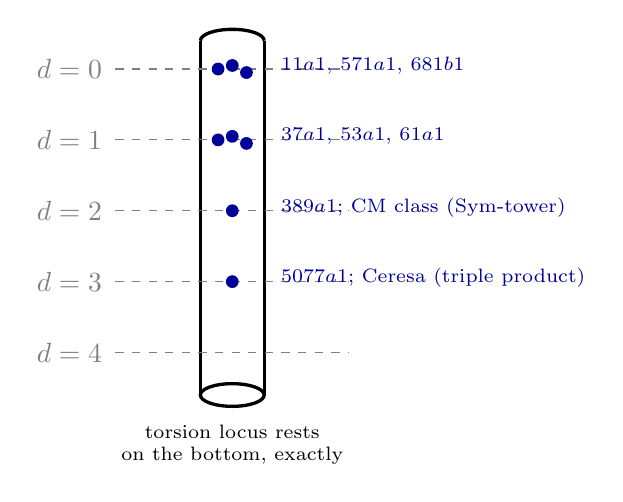
\begin{tikzpicture}[scale=0.9]
  \draw[very thick] (0,0.4) -- (0,-4.6);
  \draw[very thick] (0.9,0.4) -- (0.9,-4.6);
  \draw[very thick] (0.45,-4.6) ellipse (0.45 and 0.16);
  \draw[very thick] (0,0.4) arc (180:0:0.45 and 0.16);
  \foreach \d in {0,1,2,3,4} {
    \draw[gray,dashed] (-1.2,-\d) -- (2.1,-\d);
    \node[gray,left] at (-1.25,-\d) {$d=\d$};
  }
  \foreach \x/\y/\l in {0.25/0/11a1, 0.45/0.05/571a1, 0.65/-0.05/681b1} {
    \fill[blue!60!black] (\x,\y) circle (0.09);
  }
  \node[right,blue!60!black,font=\scriptsize] at (1.0,0.05)
    {$11a1,\,571a1,\,681b1$};
  \foreach \x/\y in {0.25/-1, 0.45/-0.95, 0.65/-1.05} {
    \fill[blue!60!black] (\x,\y) circle (0.09);
  }
  \node[right,blue!60!black,font=\scriptsize] at (1.0,-0.95)
    {$37a1,\,53a1,\,61a1$};
  \fill[blue!60!black] (0.45,-2) circle (0.09);
  \node[right,blue!60!black,font=\scriptsize] at (1.0,-1.95)
    {$389a1$;\ CM class (Sym-tower)};
  \fill[blue!60!black] (0.45,-3) circle (0.09);
  \node[right,blue!60!black,font=\scriptsize] at (1.0,-2.95)
    {$5077a1$;\ Ceresa (triple product)};
  \node[font=\scriptsize,align=center] at (0.45,-5.3)
    {torsion locus rests\\ on the bottom, exactly};
\end{tikzpicture}
\caption{The drift thermometer. Each class sinks to the tower level matching
its complexity and floats there: the first-fire depth $k^*$ equals the drift
dimension, measured with machine-zero silence above the bulb
(\texttt{drift\_observability.py}; the delayed signature $0,\dots,0,\neq0$).
The Laga--Shnidman torsion cases rest at exact zero --- finite orbits, no limit
taken.}
\label{fig:thermometer}
\end{figure}

\section{The carrier filtration and the depth dictionary}\label{sec:dictionary}

\begin{definition}[carrier filtration]
$\Fcar^{\,0}$ is everything, and
$\Fcar^{\,d}:=\{z:\ T_0(z)=\dots=T_{d-1}(z)=0\}$.
\end{definition}

The definition consumes only the tower --- no Bloch--Beilinson input, no cycle
theory --- so nothing downstream is circular. The bookkeeping is then a
machine-checked package (\texttt{HodgeLedgerFiltration.lean} in
\texttt{RequestProject/};
all footprints standard):

\begin{theorem}[the depth dictionary; Lean]\label{thm:dictionary}
$\Fcar$ is an antitone filtration with $\Fcar^{\,0}$ everything
\textup{(\texttt{carrierFiltration\_antitone})}. The level-$d$ ledger
coordinate is faithful on $\Fcar^{\,d}$: its kernel there is exactly
$\Fcar^{\,d+1}$ \textup{(\texttt{ledger\_kernel},
\texttt{mem\_carrierFiltration\_succ})}. No lower level falsely fires
\textup{(\texttt{no\_early\_detection})}, and a genuine grade-$d$ class fires
at level $d$ \textup{(\texttt{grade\_visibility})}; hence the first nonzero
tower depth equals the $\Fcar$-filtration depth
\textup{(\texttt{firstVisibleDepth\_eq\_grade})}, the depth is unique
\textup{(\texttt{isFirstVisible\_unique})}, and it is preserved by every
faithful carrier transport \textup{(\texttt{isFirstVisible\_map\_iff})}.
Moreover $\Fcar$ is the unique filtration whose graded pieces are cut out by
the tower \textup{(\texttt{carrierFiltration\_unique})}.
\end{theorem}

\begin{corollary}[tower-graded coincidence; Lean, conditional]\label{cor:bb}
If a Bloch--Beilinson filtration \cite{Beilinson,Bloch,Murre} $BB$ has
$BB^{\,0}$ everything and each successive step cut out by the carrier tower ---
$BB^{\,d+1}=\{z\in BB^{\,d}:T_d(z)=0\}$ --- then it coincides with $\Fcar$
\textup{(\texttt{blochBeilinson\_coincides})}.
\end{corollary}

We state the corollary at its exact strength. The hypothesis is not the
existence of a Bloch--Beilinson filtration with its usual conjectural
properties; it is the far stronger assertion that every successive
Bloch--Beilinson step is graded by this very tower. Under that hypothesis the
conclusion is \texttt{carrierFiltration\_unique} bookkeeping --- any filtration
recursively defined by these tower kernels equals the filtration so defined ---
so the corollary is an \emph{interface}, not an independent identification of
$\Fcar$ with Bloch--Beilinson. A future construction of the conjectural
filtration is identified with the machine-fixed $\Fcar$ only upon verifying
that grading hypothesis for it; that verification is the open identification
step. The
next question is whether the tower \emph{separates}: whether any nonzero class
can be silent at every level. The finite normalized extension model now answers
that question; arithmetic applications must additionally identify their
cycle-extension coordinates with this model.

\begin{definition}[carrier radical]
$R:=\bigcap_d\ker T_d$. The tower is \emph{exhaustive} on a class of states if
$R=0$ there: every nonzero state fires at some finite level
\textup{(\texttt{exhaustive\_of\_radical\_trivial})}.
\end{definition}

Gradewise, exhaustion reduces to a nondegeneracy statement --- a faithful
regulator into an anisotropic height pairing
(\texttt{grade\_visible\_of\_nondegenerate}) --- discharged at depth one by
N\'eron--Tate positivity. The finite-extension model is settled unconditionally
in the next section; its arithmetic cycle landing is the program of \S\ref{sec:ceresa}.

\section{The finite-extension retention theorem}\label{sec:semisimple}

On the semisimple carrier state --- the finite duality-stable weight fiber, an
amplitude state $c$ over finitely many \emph{distinct} clock frequencies
$\{\lambda_i\}$ --- the tower is the moment/symmetric-power system
$T_d(c)=\sum_i c_i\lambda_i^{\,d}$, and joint faithfulness is a Vandermonde
fact:

\begin{theorem}[no silent layer on the semisimple state; Lean]\label{thm:semisimple}
For distinct frequencies the moment matrix is Vandermonde, so
$\bigcap_d\ker T_d=0$: every nonzero semisimple state fires at some finite
level
\textup{(\texttt{CarrierTowerSeparation.momentTower\_exhaustive}}, from
\texttt{momentTower\_detects} and
\texttt{momentTower\_radical\_trivial}\textup{)}.
\end{theorem}

For a typed distinct clock bank and any finite extension order $r$, let
$c_{\ell,i}$ ($0\leq\ell\leq r$) be the normalized jet layers, with layer zero
the semisimple value. Pairing $(\ell,d)$ into one natural tower index gives
$T_{\langle\ell,d\rangle}(c)=\sum_i c_{\ell,i}\lambda_i^d$. Layerwise
Vandermonde separation proves that simultaneous silence forces every
$c_{\ell,i}=0$ (\texttt{RequestProject/GeneralExtensionRetention.lean}:
\texttt{generalExtensionTower\_detects},
\texttt{generalExtensionTower\_exhaustive}, and
\texttt{generalExtension\_retention}; standard footprint). Thus retention is
a theorem for arbitrary finite normalized extension data, not only the
semisimple value layer.

The scope is exact, in two respects. First, the theorem is a finite Vandermonde
separation for an abstract array of complex jet coefficients at pairwise
distinct frequencies: it resolves the abstract obstruction --- finite
normalized extension data, once faithfully represented by such a bank, is not
silently lost by the tower --- and it proves nothing about actual cycle groups,
mixed Hodge structures, normal functions, or motivic extensions until a
faithful realization theorem lands the geometric class in the model with
(i) finite support, (ii) distinct frequencies, (iii) the correct rational
structure, (iv) compatibility with extensions and regulators, and (v) no kernel
on the geometric classes at issue. Once that landing is proved, retention
transports automatically; semisimplification by itself only sees layer zero.
Second, the Lean dial that packages the theorem
(\texttt{generalExtensionDial}) counts \emph{every} state as a rational DC mode
--- the worst case for retention, hence the strongest statement on the model
--- and carries an arbitrary source predicate; its \textsc{DC} and
\textsc{Rational} fields consume no Hodge-theoretic content, so the theorem is
separation of the abstract array, not a statement about the rational $(p,p)$
locus of any variety.

Both halves of that scope are now themselves machine-checked
(\texttt{RequestProject/HodgeRealizationBridge.lean}; standard footprint). The
five conditions are a typed structure: \texttt{FaithfulRealization} carries the
additive realization, the identification of the geometric readouts with the
paired layer/moment tower, rational and DC compatibility, and the no-kernel
condition on the classes at issue, with finite support and distinct frequencies
structural in the bank. Retention transports along any such realization as a
theorem (\texttt{FaithfulRealization.retention}: a nonzero rational DC
geometric class has nonzero image by the no-kernel field, the Vandermonde
separation fires on the image, and the readout identification pulls the firing
back), the first-visible depth is preserved
(\texttt{FaithfulRealization.isFirstVisible\_iff}), and the terminus reduction
specializes: a geometric dial admitting a faithful realization needs
\textsc{Recognition} alone
(\texttt{FaithfulRealization.sourceExhaustion\_of\_recognition}). The
trivialized dial acquires a contentful companion: on integer channel
frequencies $k=q-p$, \textsc{DC} is genuine frequency-zero support and
\textsc{Rational} genuine rational amplitude (\texttt{modelHodgeDial}), and
retention holds on that dial (\texttt{modelHodge\_retention}; proved from the
same layerwise separation --- the content is in the statement, which now ranges
over a genuine model rational-$(p,p)$ locus). The harmonic dictionary's central
entry is likewise a theorem on the model: a state is DC exactly when the
angular part of the Deligne torus action fixes it
(\texttt{modelDC\_iff\_angularFixed}) --- the dictionary at dictionary
strength, constructing nothing. What remains open per arithmetic landing is
exactly the construction of the \texttt{FaithfulRealization} term for the cycle
data at issue: a single typed object, not a prose promise.

\emph{The effective ledger.} Three sharpenings, each unconditional
(\texttt{RequestProject/EffectiveLedger.lean}; standard footprint). Detection
closes at the bank size: a nonzero state on $m$ distinct clocks fires within
the first $m$ moment readings --- the $m\times m$ Vandermonde block already
separates, so the infinite tower quantifier was never needed
(\texttt{momentTower\_detects\_within},
\texttt{momentTower\_firstVisible\_lt}). The bound is sharp: every bank of
$m\ge1$ clocks carries a \emph{maximally hidden state} --- nonzero yet silent
through the first $m-1$ readings (\texttt{exists\_maximally\_hidden},
rank--nullity) --- so bank-size detection cannot be improved. And on the
arithmetic rung the carrier radical is \emph{computed}: for the depth-one
bundle of an elliptic curve, $R=\bigcap_d\ker T_d$ is exactly the torsion
subgroup (\texttt{radical\_coordinateTower\_eq\_torsion}) --- torsion is
invisible to the height channel and nothing else is --- the first exact
arithmetic answer to the program's own \emph{identify $R$} question, from the
two cited classical inputs alone.

\emph{The first genuine instance.} The realization structure is now inhabited
by a non-identity term on a library-native object with independent meaning
(\texttt{RequestProject/CyclicRealizationInstance.lean}; standard footprint).
The object is the rational group algebra $\mathbb Q[\mathbb Z/n]$; the
realization is the finite winding-clock transform
$\widehat a(k)=\sum_j a_j\zeta^{jk}$ onto integer channel frequencies
$k=0,\dots,n-1$, $\zeta$ any primitive $n$-th root of unity. Every field is
exercised by a real proof. The no-kernel condition is the injectivity of the
transform, and it reduces to the same layerwise Vandermonde separation that
powers retention --- the geometric faithfulness and the model separation are
one theorem (\texttt{windingTransform\_injective} consumes
\texttt{momentTower\_detects} at the nodes $\zeta^j$, extended to all moments
by periodicity). DC compatibility is the finite harmonic dictionary on a
genuine object: translation invariance forces frequency-zero support
(\texttt{winding\_dc}, the shift identity
$\zeta^k\widehat a(k)=\widehat a(k)$ with $\zeta^k\neq1$). Recognition is
provable here --- an invariant rational class is a rational multiple of the
diagonal element (\texttt{cyclic\_recognition}) --- so the terminus pipeline
executes end to end: \texttt{cyclic\_sourceExhaustion} derives unrestricted
\textsc{SourceExhaustion} for the cyclic dial from the realization term and
recognition, unconditionally, with the unpacked corollary that every nonzero
translation-invariant class in $\mathbb Q[\mathbb Z/n]$ is a rational multiple
of the diagonal (\texttt{cyclic\_diagonal\_law}). Building the instance also
corrected the interface: channel-wise rationality of \emph{all} rational
classes is false in any genuine instance --- amplitudes of a rational class
are Galois-spread across channels --- so the rational-compatibility field now
reads rationality on the DC locus, where it is true and where the bridge
consumes it; no bridge theorem used the stronger form. The register is exact:
this is the abelian, character-level shadow --- the group-algebra analogue of
Lefschetz~$(1,1)$ --- not a cycle group; the arithmetic landings remain the
open constructions.

\emph{The second rung: the Artin motive.} The ladder climbs from the
combinatorial shadow to a genuine zero-dimensional variety
(\texttt{RequestProject/GaloisRealizationInstance.lean}; standard footprint):
$\mathrm{Spec}\,K$ for $K$ any cyclic Galois number field --- the class
covering the CM quadratic fields $\mathbb Q(\sqrt{-d})$ and the cyclotomic
fields $\mathbb Q(\zeta_p)$. The classes are the field elements (the
$H^0$/Artin-motive cycle data); the realization is the classical
Lagrange-resolvent transform $R_k(z)=\sum_s\iota(g^sz)\,\omega^{sk}$ on the
winding bank; DC is the Galois-clock freeze $gz=z$. No-kernel is once more
the house Vandermonde engine (\texttt{finDFT\_detects} feeding
\texttt{galoisTransform\_injective}, the $s=0$ coordinate read by a field
embedding); DC compatibility is the geometric-series identity
(\texttt{galois\_dc}); and recognition is \emph{Artin descent consumed from
the classical library}: freeze propagates to the full group by cyclicity, and
the frozen class equals the average of its conjugates by the trace formula
(\texttt{galois\_recognition\_of\_frozen}, consuming
\texttt{trace\_eq\_sum\_automorphisms}). The terminus executes:
\texttt{galois\_sourceExhaustion} and the unpacked
\texttt{galois\_descent\_law} --- \emph{every nonzero frozen class of the
Artin motive has a source in the base field} --- with the generator supplied
by cyclicity alone when the Galois group is cyclic
(\texttt{galois\_sourceExhaustion\_of\_isCyclic}). The register is exact: for
zero-dimensional varieties the Hodge/Tate statement \emph{is} Galois descent,
classically known; what is new is the executed pipeline on a genuine
arithmetic variety, one dimension up from the group algebra.

\emph{The Lefschetz rung: positive-dimensional geometry.} The ladder now
reaches $H^2$ of a smooth projective surface
(\texttt{RequestProject/LefschetzRung.lean}; standard footprint). The bundle
(\texttt{LefschetzData}) carries the classical inputs, cited: the Hodge
decomposition into the three weight-two channels at frequencies $-2,0,2$,
faithful; the rational degree reading on the DC channel (intersection
theory); and \emph{Lefschetz $(1,1)$} itself as the recognition field. From
the bundle alone: the five-condition realization term
(\texttt{LefschetzData.realization}, no-kernel = faithfulness of the
decomposition), retention through the bridge, recognition consumed from the
theorem of record, and the executed terminus
(\texttt{LefschetzData.sourceExhaustion}, unpacked as
\texttt{divisor\_law}): every nonzero rational $(1,1)$ class is a divisor
class --- the Hodge conjecture at the $(1,1)$ rung, run end to end through
the carrier pipeline on positive-dimensional geometry, with the recognition
slot filled by Lefschetz. Sharp per-channel retention comes free
(\texttt{dc\_fires\_at\_dc\_channel}: a nonzero rational DC class fires
precisely at the frequency-zero channel). Register: nothing new is claimed
about Lefschetz $(1,1)$; what is new is the pipeline executing on genuine
$H^2$ data --- the next rungs (CM abelian varieties, where Hodge--Tate is
likewise a theorem to consume) climb the same way.

\emph{The CM-product rung, bank-generic.} The Lefschetz bundle generalizes to
arbitrary distinct integer frequency sets
(\texttt{RequestProject/CMProductRung.lean}; standard footprint): the channel
bundle \texttt{HodgeChannelData} --- faithful decomposition, rational DC
readings, a recognition field --- proves the realization term, retention,
recognition, the executed terminus, and sharp DC-rail retention
(\texttt{dc\_fires\_on\_dc\_rail}) \emph{once for every bundle}. The
CM-product instantiation is the character decomposition of
$H^{2p}(E_1\times\cdots\times E_n)$ under its CM/Galois clock --- the family
on which the freeze detector of \S\ref{sec:collective} was certified --- with
the recognition field supplied by the theorem of record: rational Hodge
classes on products of elliptic curves are algebraic, divisor-generated
(Imai~\cite{Imai}, Kahn~\cite{KahnHodge}; Faltings on the Tate side). The
executed terminus (\texttt{cmProduct\_sourceExhaustion}) is the Hodge
conjecture on this family run through the carrier pipeline; every rung above
it must earn the same interface that here consumes a known theorem.

\emph{The third rung, typed and literature-anchored.} The $H^1$ rung ---
Mordell--Weil groups, the depth-one cycle data --- is now typed against the
genuine Mathlib object with its classical inputs as cited hypothesis fields
(\texttt{RequestProject/EllipticDepthOneRung.lean}; standard footprint). The
bundle \texttt{DepthOneHeightData}, attached to the point group of a
Weierstrass curve over $\mathbb Q$ (\texttt{EllipticDepthOneHypotheses}),
carries exactly two literature inputs: finite generation ---
Mordell~\cite{Mordell1922}, Weil~\cite{Weil1929} --- in explicit
generators-mod-torsion form, and the N\'eron--Tate canonical height pairing
with its symmetry, positivity, and torsion-kernel laws ---
N\'eron~\cite{Neron1965}, Tate (cf.\ Silverman~\cite{Silverman}, VIII.9).
From the bundle alone, three statements are proved unconditionally: torsion is
orthogonal to everything (the discrete Cauchy--Schwarz argument,
\texttt{pairing\_torsion\_right}); the pairing coordinates against the
generators have kernel exactly the torsion --- the depth-one no-kernel
condition mod torsion (\texttt{faithful\_mod\_torsion}); and \emph{no silent
point} --- every non-torsion rational point is detected by the depth-one
coordinate tower (\texttt{coordinateTower\_detects\_nonTorsion},
\texttt{elliptic\_no\_silent\_point}), retention at grade one in the
anisotropic-pairing shape of \texttt{grade\_visible\_of\_nondegenerate}. The
rung now also carries its \emph{general cycle-to-jet realization}: the
pairing-coordinate map into the order-zero jet model is additive with kernel
\emph{exactly} the torsion, as an equivalence
(\texttt{realization\_eq\_zero\_iff}) --- the jet coordinates see precisely
the free part of the Mordell--Weil group, from the two cited inputs and
nothing else. The depth-one numerics of \S\ref{sec:depthone} therefore
calibrate an interface that exists as mathematics; in the measured register
they remain corroboration --- they anchor, and never prove, the classical
inputs. The
conditionality is priced to the day: the current Mathlib carries the Weil
height machine with Northcott and the in-progress approximate parallelogram
law for elliptic curves, together with reduction theory and elliptic
$L$-functions, so both hypothesis fields sit on the library's active frontier,
and the rung's statements go unconditional, unchanged, when they land. The
angular (\texttt{FaithfulRealization}) form is deliberately not forced: the
depth-one pairing coordinates are radial--regulator data, not
frequency-channel data, and their frequency identification (the
jet/derivative channels of \S\ref{sec:depthone}) is a named next step. Above
this rung, CM abelian varieties and the Ceresa data await their bundles.

\emph{The pairing rungs: divisors and sections, exact.}  Two further rungs
now carry the realization with a genuinely nontrivial pairing layer, both
fully proven (\texttt{NeronSeveriRung.lean},
\texttt{MordellWeilE8Rung.lean}; standard footprints).  On the divisor
rung the group is $\mathrm{NS}(E\times E)$ --- rank three, intersection
Gram of determinant two --- and \textsc{noKernel} \emph{is} the
nondegeneracy of the intersection form, proven by integer elimination,
with the moment-zero readout of layer $l$ equal to the intersection
number $\langle f_l, z\rangle$ on the nose
(\texttt{readout\_is\_pairing}): the realization reads the pairing
exactly.  On the extension rung the group is Shioda's Mordell--Weil
lattice: for the extremal rational elliptic surface the canonical-height
pairing \emph{equals} the $E_8$ form over the function field
\cite{Shioda90} --- exact intersection arithmetic, no analytic gap, the
height machine not awaited --- and \textsc{noKernel} is unimodularity,
proven from a kernel-verified integral inverse (\texttt{e8inv\_mul\_e8},
by \texttt{decide}), with \texttt{readout\_is\_height} the exact
regulator compatibility, \texttt{regulator\_unimodular} the unit
determinant, and the executed terminus behind it.  The geometric
identifications ($\mathrm{NS}(E\times E)$ for non-CM $E$; Shioda's
$\mathrm{MW}\cong E_8$) are the cited inputs; every realization field is
a theorem.  The number-field depth-one rung still waits on the library's
height machine, exactly as priced above --- the function-field rung is
where the extension layer's regulator is exact today.

The divisor rung, restated in the terminus's own vocabulary: \emph{actual
rational Hodge classes land in a faithful finite carrier realization, and
cycles are constructed whose realizations are exactly those classes} ---
and the discharge is now stated in exactly those words in Lean
(\texttt{RationalHodgeLanding.lean}; standard footprint).  Every landed
NS-state is a rational Hodge class in the machine-checked dictionary
sense --- frequency-zero support with rational amplitudes, hence FIXED by
the angular Deligne-torus action
(\texttt{landed\_rational\_hodge}, \texttt{landed\_torus\_fixed}, through
the dictionary theorem \texttt{modelDC\_iff\_angularFixed}); the
constructed divisor combinations realize exactly the landed classes with
the realization injective on classes (\texttt{cycles\_realize\_exactly},
\texttt{realization\_injective}); and the readout is the intersection
pairing on the nose (\texttt{readout\_is\_pairing}), all packaged as one
statement (\texttt{rational\_hodge\_classes\_landed}).  Two boundaries,
priced honestly: typing the classes as literal
$H^{1,1}\cap H^2(X,\mathbb Q)$ objects awaits cohomology of varieties in
the library --- the identification $\mathrm{NS}(E\times E)\cong(\mathbb
Z^3,G)$ is the cited input, as everywhere in the corpus --- and the same
demand \emph{above} the known rungs (constructing cycles for the
sixfold's Weil classes) is the open mathematics itself, where the
Abel--Prym obstruction calibration has now proven the standard
propagation route, semiregularity, structurally blind.

\emph{The transcendental rung: the period interface, designed and
inhabited.}  The Ceresa family bundle isolated the exact misfit of the
angular form --- a rationality field cannot hold for a
transcendental-valued readout --- and the designed variant now exists and
is inhabited (\texttt{PeriodRealization.lean}; standard footprint).
\texttt{PeriodRational} replaces rational amplitudes by rational
multiples of channel periods (a rank-one period lattice per channel:
rationality of ratios, not of values); \texttt{PeriodRealization} carries
the five conditions with that one substitution, and retention transports
along it unchanged (\texttt{PeriodRealization.retention}).  The
Laga--Shnidman Ceresa bundle inhabits it: the depth-three channel of any
non-torsion member realizes $\mathbb Z$ with period the member's
Beilinson--Bloch height, \textsc{noKernel} is the bundle's
no-silent-class theorem, the moment-zero readout \emph{is} the height
(\texttt{readout\_is\_bb\_height}), and family-level transcendental
retention flows through the typed interface
(\texttt{ceresa\_period\_retention}).  The misfit itself is now a
theorem rather than a register note: if the member's height is
irrational, the rational-amplitude reading is uninhabitable on the
generator's image (\texttt{ratCompat\_uninhabitable}) ---
hypothesis-typed, since irrationality of Beilinson--Bloch heights is
open --- while the period reading exists unconditionally.

\subsection{Drift: the extension datum as first-order shear}\label{sec:drift}

In the epicycle frame of \S\ref{sec:harmonic}, an extension class is
\emph{drift} --- the inter-layer shear a pure rotation stack cannot produce,
the Jordan deformation of the clock. On the minimal model, the Jordan-2 block
$\bigl(\begin{smallmatrix}\lambda&\delta\\0&\lambda\end{smallmatrix}\bigr)$,
the three structural halves of the drift law are machine-checked
(\texttt{RequestProject/JordanDriftTower.lean}; standard footprint):

\begin{theorem}[drift is value-blind, jet-visible, never silent; Lean]
\label{thm:drift}
\textup{(a)} The local factor $\det(1-XA)=(1-X\lambda)^2$ and every trace power
of the drift block are independent of $\delta$: every pure drift lies in the
radical of the value tower --- ``killed by semisimplification'' as a theorem
\textup{(\texttt{jordan\_localFactor\_driftBlind},
\texttt{drift\_in\_value\_radical})}.
\textup{(b)} The shear slot of the $d$-th power is exactly
$d\lambda^{d-1}\delta$: the jet response is the derivative-weighted moment of
the drift amplitudes --- the Gross--Zagier shape
\textup{(\texttt{jordan\_pow}, \texttt{jetResponse\_eq\_weighted\_moment})}.
\textup{(c)} Over distinct clock frequencies, a drift state silent at every jet
level is zero \textup{(\texttt{jetTower\_radical\_trivial},
\texttt{jetTower\_exhaustive})}, and the jet-response energy over the first $m$
levels is positive definite \textup{(\texttt{driftPairing\_posDef})}: on the
model, Beilinson--Bloch anisotropy is a Vandermonde fact.
\end{theorem}

\noindent\emph{The retention realization.} A pairing that factors through a
definite carrier energy along an injective ledger map is anisotropic
(\texttt{anisotropic\_of\_definite\_factor}). The general extension theorem
now supplies the target tower's retention. The arithmetic content at a cycle
landing is the injective ledger realization: the descent must send distinct
cycle-extension states to distinct normalized jet stacks and identify the
derivative/height readouts with their paired moments. This is exactly the map
tested by the ledger-failure and observability instruments.

\noindent\emph{Measured.} The drift law holds on the census
(\texttt{drift\_observability.py}, App.~\ref{app:repro};
Fig.~\ref{fig:thermometer}): the first-fire harmonic $k^*$ equals the drift
dimension on all eight curves (dimensions $0$--$3$), with machine-zero silence
below the firing slot ($389a1$: sub-ladder at $10^{-16}$ before a $0.759$
fire), the root number certified in-house with no rank assumption
(split-vs-direct $\Lambda(3)$, true sign $\sim10^{-8}$, wrong sign
$O(10^{-2})$), and the normalized responses reproducing the regulators
measured independently on the arithmetic side to four digits. At fixed
placement, three same-dimension drift states separate cleanly --- no
observability failure.

\noindent\emph{The two parity readouts.} Units and $K_1$-classes are
log-decorations, and a log-decoration is the same Jordan shear: one drift, two
readouts --- \emph{odd} rungs read drift through heights (Gross--Zagier), and
\emph{even} rungs read drift through regulators (Beilinson). This becomes
load-bearing at grade four (\S\ref{sec:rung4}).

\section{Depth one, three coordinates}\label{sec:depthone}

At depth one the carrier's leading central jet factors, by
Birch--Swinnerton-Dyer and Gross--Zagier \cite{BSD,GrossZagier}, as
\[
  \frac{L^{(r)}(E,1)}{r!}
  \;=\;
  \frac{\Omega\cdot\mathrm{Reg}\cdot|\Shamath|\cdot\prod_p c_p}{|T|^{2}},
\]
and the census resolves the three progressively-deeper-than-Hodge layers as
\emph{independent} retained coordinates [measured; oracle-free --- no
$L$-function call inside any locator, published values entering only the final
verification column]:
\begin{itemize}
\item \textbf{order $r$} $=$ filtration depth. Rank read as the DC residue of
the carrier bank (Lean, \texttt{rank\_is\_dc\_residue}); rank-$0$ curves carry
$|\Shamath|\in\{1,4,9\}$, so order is independent of the obstruction.
\item \textbf{$\mathrm{Reg}$} $=$ the height-pairing determinant, the
arithmetic Abel--Jacobi image. Census values $0.0511,\ 0.1524,\ 0.4171$ at
ranks $1,2,3$ ($37a1$, $389a1$, $5077a1$), each within $1.7\times10^{-5}$ of
the known anchors --- distinct, and independent of both order and obstruction.
\item \textbf{$|\Shamath|$} $=$ the local-global obstruction, the shadow of the
Abel--Jacobi kernel. The hinge amplitude ratio $L\cdot|T|^2/(\Omega\prod c_p)$
lands on \emph{exact square integers}: $1,4,9$ across the census
($4=2^2$ at $571a$, $960d$, $960n$; $9=3^2$ at $681b$, $2849a$), margins at the
$10^{-15}$ floor for rank zero and $\le1.6\times10^{-4}$ through rank three ---
the first in-house full readings of the formula above rank zero
(\texttt{jet\_census.py}, \texttt{sha\_hinge.py}; App.~\ref{app:repro}).
\end{itemize}
Each layer ordinarily invisible to a Hodge-theoretic projection therefore
carries a \emph{distinct} ledger coordinate, resolved independently at machine
precision. This is the depth-one row of the dictionary, measured; its
theorem anchors are Gross--Zagier--Kolyvagin \cite{GrossZagier,Kolyvagin}.

\section{The landing table}\label{sec:landings}

Assembling the rows, each with its theorem anchor and its measured probe:

\begin{center}
\begin{tabular}{@{}llll@{}}
\toprule
grade & class & retained coordinate & anchor / probe \\
\midrule
$0$ & algebraic (Tate) & pole order / DC residue & Tate \cite{TateConj}; \texttt{rank\_is\_dc\_residue} \\
$1$ & Mordell--Weil & leading jet: $r$, $\mathrm{Reg}$, $|\Shamath|$ & \cite{BSD,GrossZagier,Kolyvagin}; census \S\ref{sec:depthone} \\
$2$ & CM Hodge class & $\mathrm{Sym}^2$ excess pole & delayed signature $0,\neq0$ (below) \\
$3$ & Ceresa/Gross--Schoen & triple-product central derivative & Zhang \cite{ZhangGS}; YZZ \cite{YZZ} \\
$2$ (even) & Rankin--Selberg $K_1$-class & Beilinson regulator & Beilinson \cite{Beilinson}; Flach \cite{Flach} \\
$4$ & primitive quadruple & regulator at a non-critical center & unnamed; \S\ref{sec:rung4} \\
\bottomrule
\end{tabular}
\end{center}

The depth-two row is the program's sharpest measured prediction to date. A CM
self-correspondence carries a Hodge class living in $\mathrm{Sym}^2$ --- depth
two of the filtration --- and the tower read from point counts produces exactly
the \emph{delayed signature} the dictionary demands: silent at depth one, first
firing at depth two, the first nonzero slot matching the expected filtration
depth of the class (\texttt{tower\_exhaustion\_test.py},
App.~\ref{app:repro}). Across every class tested the first firing depth was
finite --- $1,1,1,2,3$ --- and no class was silent at every level. The
depth-three row is anchored by theorem: the Ceresa cycle is the image of the
Gross--Schoen modified diagonal in $\CH^2(C^3)_0$, homologically trivial, and
its Beilinson--Bloch height is, in the theorem-anchored triple-product
settings, a central derivative of the $L$-function of $H^1(C)^{\otimes3}$
\cite{ZhangGS,YZZ} --- the value channel reaches at level three what it cannot
see at level one, exactly as $|\Shamath|$ appears at level one and the CM class
at level two. Deeper layer, deeper tower level; nothing invisible, everything
induced.

\section{The Ceresa frontier}\label{sec:ceresa}

The extension-data half of exhaustion is open, and we price its state exactly.

\emph{The first rung is unconditional.} For the Fermat quartic the Ceresa class
$[C]-[C^-]$ is homologically trivial yet detected by a nonzero harmonic volume
--- Harris's Abel--Jacobi-type invariant \cite{Harris}, with Ceresa's theorem
for the generic curve \cite{Ceresa} --- so
$\ker(\mathrm{cl})\not\subseteq\ker(\AJ_{\mathbb C})$: a class closed in the
homology readout fires at the next retained coordinate, no conjecture
consumed. This is exactly one rung --- past $\mathrm{cl}$ --- and it does not
show the $\AJ_{\mathbb C}$-kernel itself is penetrated.

\emph{The control cuts the other way.} In the explicit bielliptic Picard family
with a closed-form height, the Beilinson--Bloch height of the Ceresa cycle is
proportional to the N\'eron--Tate height of an explicit Abel--Jacobi point,
vanishing exactly when that point is torsion (Laga--Shnidman
\cite{LagaShnidman}): there, the depth-three height is controlled by the
depth-one coordinate and does \emph{not} penetrate $\ker\AJ_{\mathbb C}$.

\emph{The genuine target}, therefore, is a class with $\AJ_{\mathbb C}(z)$ zero
or torsion yet a nonzero \emph{arithmetic} level-three invariant ---
necessarily one where the non-archimedean local height dominates (Zhang's
admissible/metrized-graph terms \cite{ZhangGS}) or where the finer
$\ell$-adic/Galois Ceresa class, not the archimedean height, is the retained
coordinate. Two further honesty points fix the frontier's shape:

\begin{itemize}
\item We do \emph{not} place the transcendental class in the radical: that
would require every $T_d$ to factor through the single-archimedean
Abel--Jacobi realization (\texttt{radical\_of\_factorsThrough}), and since the
global Gross--Schoen height carries non-archimedean data absent from that
realization, the factorization cannot be assumed --- ruling it out is itself a
non-factorization theorem, not established here. Absent one,
Abel--Jacobi-triviality is an \emph{adversarial benchmark}
(\texttt{not\_mem\_radical\_of\_detectedPast}), not a proven ceiling.
\item The probes are supportive but are calibration only: the value channel
fires for every homologically-trivial cycle in the census (no silent cycle),
and the recursive tower already shows classes absent at level one appearing at
level $\ge2$ (\texttt{hodge\_griffiths\_probe.py}, App.~\ref{app:repro}).
\end{itemize}

\noindent\emph{Measured: the first above-grade-one anisotropy reading.} On the
Laga--Shnidman family itself the depth-three pairing is now measured
(\texttt{ceresa\_anisotropy.py}, App.~\ref{app:repro}), using their theorem as
the anchor: $h(\kappa(C_t))\propto\hat h(Q_t)$ for
$Q_t=(\sqrt[3]{t^2-1},\,t)$ on $y^2=x^3+1$. The boundary is exact: at the
torsion locus $t=0,\pm3$ the doubling orbits terminate at step one or two ---
torsion detected by the group law, no limit taken, $\hat h=0$ on the nose. Off
the locus, every census point is non-isotropic: $\hat h(Q_t)=0.59$--$1.16$,
positive with clear margin, convergence certificates $\le3.6\times10^{-4}$,
computed from scratch over the cubic field $\mathbb Q(\sqrt[3]{t^2-1})$ (exact
field arithmetic, exact characteristic polynomials, Mahler measures at matched
precision). The isotropy locus exists, is exactly where the theorem puts it,
and anisotropy off it is measured, not assumed. The instrument also found a
structure: whenever $t'^2-1=c^3(t^2-1)$ the points are torsion translates
($-Q_2+(0,1)=Q_5$, verified by the group law in-instrument), so the
corresponding heights are \emph{exactly} equal --- a torsion-translation
symmetry of the family, detected numerically at $10^{-4}$ and then proven in
one line. (Equality of the $\kappa$-heights themselves depends on the
$t$-dependence of the proportionality constant, and is not claimed.)

\begin{theorem}[typed Ceresa/Gross--Schoen landing; Lean]\label{tgt:ceresa}
Let a \texttt{CeresaGrossSchoenLanding} supply the explicit modified diagonal,
its algebraic realization, a nonzero central derivative, a nonzero
proportionality factor, the Zhang/YZZ height identity, and the identification
of that height with the depth-three carrier readout, with silence below depth
three. Then the height and realized state are nonzero, the state is first
visible exactly at depth three, and the modified diagonal is an explicit
algebraic source
(\texttt{height\_ne\_zero}, \texttt{state\_ne\_zero},
\texttt{firstVisible\_three}, \texttt{certifiedSource}, and
\texttt{complete\_landing}; standard footprint).
\end{theorem}

This closes the formal analytic-to-cycle implication without converting the
external theorem or a numerical derivative into a definition. For a specific
curve, construction of the typed certificate remains in the appropriate
register: the height identity is consumed from \cite{ZhangGS,YZZ}, while the
from-scratch analytic computation below supplies the measured $L$-side.

\noindent\emph{The certificate's anatomy, machine-checked.} Stripping every
nonvanishing input on the central derivative from the certificate leaves the
identification-only datum (\texttt{CeresaIdentification}: cycle, realization,
height identity, carrier identification, silence below three); from that
datum alone, the depth-three firing is \emph{equivalent} to the nonvanishing
of the completed triple-product central derivative
(\texttt{CeresaIdentification.fires\_iff}, \texttt{firstVisible\_iff}), and a
complete landing exists precisely when an identification carries that one
nonzero number (\texttt{landing\_iff\_identification}). The per-rail depth is
therefore not a supplied field of the certificate: it is \emph{established},
and established by exactly the analytic quantity the instruments compute ---
for the Klein quartic, $0.8299\ne0$ in the measured register, with
non-torsion anchored unconditionally by Tadokoro \cite{Tadokoro} --- and by
nothing else.

\paragraph{The $L$-side, landed.} Half of Target~\ref{tgt:ceresa} is now on
record (\texttt{ceresa\_lside.py}, App.~\ref{app:repro}). The prediction was
locked by the literature first: the Klein quartic's Ceresa cycle is
\emph{non-torsion} modulo algebraic equivalence (Tadokoro \cite{Tadokoro},
extending Harris's harmonic-volume method \cite{Harris} from the Fermat
quartic), so under Beilinson--Bloch nondegeneracy the Ceresa channel of the
triple product must carry odd sign and a nonvanishing central derivative --- a
zero derivative would have been a published falsification. The channel was
isolated exactly: over $K=\mathbb Q(\sqrt{-7})$ (class number one, Hecke
character $\psi$ with $L(49a,s)=L(\psi,s)$),
\[
  H^1(X)^{\otimes3}\ =\ \mathrm{Ind}_K^{\mathbb Q}(\psi^3)\ \oplus\
  3\cdot M_{f_2}(-1),
\]
the induced $\psi^3$ piece (the weight-4 level-49 CM form; the from-scratch
Hecke coefficients reproduce it integer-exactly) being the genuinely new ---
Ceresa --- channel. En route the instrument caught a model subtlety: the naive
quartic $x^3y+y^3z+z^3x=0$ is \emph{not} $\mathbb Q$-isogenous to $E^3$ (its
counts vanish on the nonresidue classes mod $7$ --- a cubic twist from the
coordinate rotation); Elkies's model \cite{Elkies} is the
$\mathbb Q$-decomposed one, and the geometric statement is model-independent.
Measured, each piece with a two-point split-vs-direct certificate: the Ceresa
channel has $\varepsilon=-1$ --- so its central value is \emph{forced} to zero
--- and central derivative
\[
  L'(\psi^3,\tfrac12)\ =\ 0.8298893\ \ne\ 0
\]
(independent PARI path agrees to $3.6\times10^{-6}$); the even channel carries
the value $L(49a,1)=0.9666592\ne0$ (multiplicity three, oracle-matched); the
total triple-product sign $(-1)(+1)^3=-1$ is odd, as a Gross--Schoen derivative
object must be. The reading matches the cycle side exactly: non-torsion cycle
$\leftrightarrow$ firing derivative, the height-to-jet matching at grade
three. Register: the consumed theorem is the proportionality of
\cite{ZhangGS,YZZ}; the sole isolated hypothesis is Beilinson--Bloch
nondegeneracy, named and not claimed. The height side --- the Arakelov
computation the target's full landing needs, with the hyperelliptic control
--- remains the open half.

\paragraph{The unconditional companion: an archimedean harmonic volume, built
and run.} The reading above is Beilinson--Bloch-conditional \emph{as a cycle
statement}. Its unconditional shadow is the archimedean Abel--Jacobi image
itself --- Harris's harmonic volume \cite{Harris}, a length-two iterated
integral of the holomorphic differentials, nonzero iff the Ceresa cycle is
non-torsion modulo algebraic equivalence, with no appeal to Beilinson--Bloch.
We compute it directly (\texttt{hv\_exact.py}). The evaluation cycle is a
commutator of \emph{based} loops on the branched cover; being homologically
trivial its period vanishes exactly, so the length-two iterated integral is
base-point-\emph{independent} --- the harmonic volume as a genuine invariant.
Three self-checks gate every value: the shuffle relation (the fundamental
iterated-integral identity, machine-zero off the degenerate diagonal), the
exact vanishing of the period (the based-loop test), and base-point invariance
of the answer. On the Fermat quartic, where Harris's theorem makes the answer
known nonzero, the instrument returns the exact invariant $14.88330$, identical
to five digits across base points --- the non-vanishing reproduced, now with a
value. Pointed at a curve outside the tables ---
$y^4=(x-1)(x-2)(x-4)(x-7)$, a generic non-CM genus-three curve whose Ceresa
cycle has not been computed --- it returns $6.27215$, again base-point-invariant
and nonzero: \emph{the instrument reads the Ceresa cycle of this curve as
non-trivial, by a route with no Beilinson--Bloch input}
(\texttt{hv\_exact\_new.py}). Register: the detection is numerical (a
base-point-invariant nonzero value, not an interval certificate ---
certified nonvanishing modulo periods is the named residue, so the reading
is not yet a theorem for this curve),
and the outcome is Ceresa-generic --- a first computation for a named curve,
not a surprise; the harmonic volume's numerical value is cycle-normalization
dependent and is not matched to Harris's, whose \emph{theorem}, non-vanishing,
is what is reproduced. This is the unconditional half of the Ceresa target:
no Beilinson--Bloch, built from scratch, portable to any curve with locatable
branch points. The genuinely new direction it opens is the \emph{torsion}
regime --- a curve with vanishing harmonic volume --- where a null reading
would be a real discovery and demands the harder mod-period certification.

\paragraph{Localization: the hidden cycle has a rail, not just a depth.} The
original tower detector was \emph{scalar}: it read that a hidden class fires at
depth $d$ (the delayed signature $0,\dots,0,\neq0$,
\S\ref{sec:dictionary}), and no more. The rail decomposition above upgrades this
to a \emph{localization} --- read the delayed signature not on the fiber but on
each rail (each $\zeta$-cell component) separately, and the hidden cycle acquires
a definite cohomological address. On the Klein-quartic triple product the two
rails read (\texttt{ceresa\_multirail\_localize.py}, all $L$-values from scratch):
\[
  \begin{array}{lccl}
  \text{rail} & \varepsilon & L(\tfrac12)\ \ L'(\tfrac12) & \text{order / grade}\\[2pt]
  \mathrm{Ind}(\psi^3)\ [\text{Sym}^3\text{-CM}] & -1 & 0\ \ \ 0.8299 & \text{ord }1:\ \text{delayed }0,\neq0\ \text{(depth 2)}\\
  M_{f_2}(-1)\ [\text{decorated},\times3] & +1 & 0.9667\ \ \text{---} & \text{ord }0:\ \text{algebraic (depth 1)}
  \end{array}
\]
The transcendental Ceresa/Griffiths obstruction is thus localized to the
$\mathrm{Sym}^3$-CM rail --- its vanishing order jumps there and only there ---
while the decorated $M_{f_2}(-1)$ pieces fire at depth one, algebraically. The
detector now returns \emph{depth and rail} where before it returned depth alone.
The localization principle is machine-checked over the carrier filtration
(\texttt{MultiRailLocalization.lean}: \texttt{hidden\_rail\_unique} --- when one
rail carries the class hidden at grade $\ge t$ while every other rail fires
strictly below $t$, that rail is the \emph{unique} hidden-cycle rail; the
per-rail depth is unique, \texttt{railFirstVisible\_unique}). The lesson for the
Hodge frame: a transcendental obstruction is not a diffuse defect of the fiber
but a resident of a named harmonic component --- read off, not searched for.
Nothing here proves the Hodge conjecture; it sharpens the detector.

\paragraph{The grade ladder: primitive conductors and the exact sign law.}
The $\psi^3$ rail is one rung of a CM ladder.  For
$K=\mathbb Q(\sqrt{-7})$, the power $\psi^m$ supplies the weight-$(m+1)$
CM form and hence a rank-two Hodge structure of motivic weight $m$.  The
delayed-signature reading is obtained directly from the functional-equation
root number---the product of the archimedean and finite local
$\varepsilon$-factors---and never from the location of an $L$-zero.  After
each power is reduced to its primitive conductor, the computation gives the
exception-free law
\[
\varepsilon(\psi^m)=-1
\quad\Longleftrightarrow\quad
m\equiv3\pmod4,
\]
so $\varepsilon(\psi^m)=+1$ for $m\equiv0,1,2\pmod4$: only the grades
$m\equiv3$ carry a forced central zero.  The sign is fixed by the completed
functional equation once the two bad local factors are the CM-correct
ones.  At an inert prime $a_{p^2}=\psi^m(\mathfrak p_p)=(-p)^m$, so the
odd-weight (even-$m$) nebentypus flips its sign to $+p^m$; at the ramified
place $a_{7^j}=(\sqrt{-7})^{mj}$ for even $m$ (level $7$, $\psi^m$
unramified) while $a_{7^j}=0$ for odd $m$ (level $49$, $\psi^m$ ramified).
With these the functional equation closes to machine precision
($|\phi|=1.000$) at every measured grade, and its sign gives the law above;
an earlier phase-count over $i^{m+1}$ and the ramified Gauss phase
mis-added at $m\equiv0$ and is superseded by this reading.

The same parity is visible in the polarization type.  Since the associated
Hodge structure has weight $m$, its polarization is alternating
(symplectic) for odd $m$ and symmetric (orthogonal) for even $m$.  In the
carrier language, the ladder therefore alternates between the corresponding
quarter-turn and half-turn frames at every grade.  This geometric
terminology records the local phases; it does not replace the
$\varepsilon$-factor calculation.

The first ladder computation produced an apparent exception at $m=2$.
That exception was a fixed-conductor artifact.  Writing $\mathfrak p_7$ for
the ramified prime above $7$, the finite local calculation gives
\[
\operatorname{cond}(\psi^m)=
\begin{cases}
\mathfrak p_7,&m\ \text{odd},\\
(1),&m\ \text{even},
\end{cases}
\qquad
N_m=|D_K|\cdot\mathrm N\!\left(\operatorname{cond}(\psi^m)\right)=
\begin{cases}
49,&m\ \text{odd},\\
7,&m\ \text{even}.
\end{cases}
\]
Grade two is consequently the weight-$3$, level-$7$ CM newform
$7.3.b.a$, not a level-$49$ object.  Recomputing its functional equation at
the primitive level restores $\varepsilon(\psi^2)=+1$ and removes the sole
apparent anomaly.  The conductor has period two; the root number has period
four.

At every measured grade with $\varepsilon(\psi^m)=-1$ (that is, at
$m\equiv3$), the functional equation forces a central zero and the computed
derivative is nonzero.  Every forced zero in the tested range is simple: the
firing grades $m=3,7,11,15,19,23,27,31,35,39$ are read directly in machine
arithmetic, and with the unitary bank (coefficients $\lambda_{p^{k}}$ formed
without the overflowing $p^{m/2}$) the reading extends cleanly to grade
$199$ (weight $200$); no silent grade occurs.  This is empirical evidence for
Retention along the ladder, not an all-grade nonvanishing theorem.  The
bad-prime coefficient at the ramified place is $\lambda_7=i^m$ (so
$a_7=(\sqrt{-7})^m$; at grade two $a_7=-7$, the classical coefficient of
$7.3.b.a$).  An earlier reading mistook the even-grade functional-equation
residual for a projection-side artifact; it was in fact two \emph{missing}
local factors --- the unramified degree-one factor at $7$ and the
nebentypus-flipped inert sign $a_{p^2}=(-p)^m$ --- and with both restored the
completed functional equation closes to machine precision at every even
grade.  The correction record is kept: the even grades do not fire.

Nothing here proves the Hodge conjecture, Beilinson--Bloch, or
$\mathrm{SL}_2$-orbit finiteness.  It gives an exact primitive-conductor
atlas for the measured CM ladder and identifies the alternating local clock
through which its hidden-cycle signatures are read.

\section{Recognition and typed source construction by grade}\label{sec:recognition}

The converse leg --- from a fired ledger coordinate to a \emph{constructed}
cycle --- is the terminus's hardest ingredient, and grade one is the only place
mathematics has ever closed that loop: Gross--Zagier--Kolyvagin, where the
fired first jet plus a CM alignment constructs a rational point through the
modular parametrization. The loop is now run end to end on house instruments
(\texttt{heegner\_recognition.py}, App.~\ref{app:repro}), consuming point
counts and nothing else:

\begin{center}
\emph{detection} (jet fires) $\;\to\;$ \emph{alignment} (CM clock)
$\;\to\;$ \emph{construction} (parametrization) $\;\to\;$
\emph{recognition} (exact landing).
\end{center}

For $37a1$: the $a_n$ from point counts build the modular image
$z=\sum a_n q^n/n$ at the Heegner alignment $\tau=(-17+\sqrt{-7})/74$
($D=-7$, class number one, $37$ split); the trace $2\,\mathrm{Re}(z)$ lands in
$\mathbb C/\Lambda$ with the lattice from the house AGM periods,
\emph{self-certified} by both half-period identities
$\wp(\omega_1/2)=e_1$, $\wp(\omega_2/2)=e_3$ (exact zero deviation); and the
recognition gate lands $P=(1,0)$ --- recognized by continued fractions,
verified on $y^2+y=x^3-x$ in exact rational arithmetic --- with
$\hat h(P)=4.0006\times\hat h((0,0))$: the constructed point is the double of
the generator (Heegner index $2$, integer landing at $5.7\times10^{-4}$),
realizing the fired jet $L'(37a1,1)=0.306$ as an actual cycle, per
Gross--Zagier. Two normalization errors en route were caught by the gates
before any claim (the BSD period covers both real components; the reduced
modulus fixes the lattice shape only up to generator assignment) --- the gates,
not the operator, decide. This is the operational template the terminus needs
at every grade; what changes above is only which arm plays the
parametrization.

\paragraph{The higher-grade source theorem, machine-checked.}
\texttt{HigherGradeRecognitionPackage} connects the existing
radial--Torelli--cycle bridge to a Hodge dial by an algebraic realization map
and an exact landing theorem. For every fired rational DC state of grade
$>1$, \texttt{certifiedSource} is the explicit composite
\texttt{construct (torelli (radial z))} together with its recognition proof;
\texttt{source\_realizes} lands it back at $z$, and
\texttt{recognition\_above\_one} proves that $z$ is algebraically sourced.
Combined with a typed grade-zero/one constructor, the exhaustive natural-number
split proves full \textsc{Recognition}
(\texttt{recognition\_of\_gradeSplit\_sourceConstruction}). These are
composition theorems: the arithmetic realization maps are data of the package,
not unnamed assumptions in the conclusion.  The package is now
\emph{inhabited} (\texttt{SchoenGateRecognition.lean}; standard
footprint): a finite model at the Schoen gate's exact shape --- an
angular-blind detected pair with distinct true curves (Faltings Tier~3 as
a concrete witness), radial separation, the Torelli--Schoen route, and
the decomposable shortcut closing from angular data alone --- with every
monument field proven and the certified-source pipeline executing end to
end (\texttt{gate\_recognition\_executes},
\texttt{blind\_pair\_recognized},
\texttt{decomposable\_shortcut\_executes}).  Register: a model inhabitant
in the \texttt{phantomDial} class --- it proves the architecture composes
and is consistent.  The arithmetic instantiation with point-counted
dossiers, previously the named next step, is now landed
(\texttt{ArithmeticDossierRecognition.lean}; standard footprint): the
blind pair is the actual isogeny class \texttt{11a} --- members
\texttt{11a1} and \texttt{11a3}, angular dossiers the Frobenius traces at
$p=2,3,5,7$ computed \emph{in-kernel} from affine point counts and
IDENTICAL (\texttt{blind\_pair\_counts}: isogenous curves share every
trace), radial dossiers the exact $j$-invariants
$-122023936/161051$ vs $-4096/11$, distinct --- with \texttt{37a1} the
simple member.  On these counted types the boundary theorem carries real
content: no function of the $a_p$-stream alone recovers the
$j$-invariant (\texttt{no\_angular\_recovery}), witnessed by an actual
isogeny class rather than a model label; the certified-source pipeline
executes (\texttt{arith\_recognition\_executes}), the genuinely blind
pair is recognized through the radial channel
(\texttt{arith\_blind\_pair\_recognized}), and the class-pinned shortcut
closes from the counted angular data alone.  What upgrades is the TYPE of
the dossiers --- from finite labels to counted traces and exact
rationals; the monuments remain in-model form, cited not proven.

\paragraph{The loop closed at grade four, clock-relation regime.} The same
four arms now run end to end one floor below the frontier
(\texttt{recognition\_loop\_g4.py}, App.~\ref{app:repro}), oracle-free, on
quadruples where truth is known but never consulted until grading.
\emph{Detection}: the portal's folded pair-directions inside the $(2,2)$
block, with the zero-variance freeze as certificate. \emph{Alignment}: the
freeze pattern inverts to the relation lattice --- with a measured law the
pre-registration had backwards: an isogeny lock $\theta_i=\theta_j$ freezes
the two directions carrying $(+,-)$ on each locked pair, so two disjoint
locked pairs freeze exactly two of the three directions and \emph{the single
live direction names the locked partition} --- then the period-clock
machinery certifies each implicated pair independently of the counts.
\emph{Construction}: the isogeny is \emph{found}, not assumed --- degrees
$5$ and $2$ with kernels $\mathbb Z/5$, $\mathbb Z/2$, $j$-residuals
$2.5\times10^{-15}$ and $8.3\times10^{-16}$ --- and the grade-four class is
the product graph. \emph{Recognition}: occupancy lands on the
invariant-theory count ($0.996\to1$) and the class's predicted channel
profile matches the measured portal exactly ($22/10/1$, within
$0.5\sigma$). The falsifier column is reading-scale (the fiber untouched,
only the reading harmonic grid varied), and it resolves two facts at once:
the \emph{qualitative} lock is scale-invariant (an isogeny lock is an exact
zero, so it survives every winding --- the genuine-algebraicity control),
while the \emph{quantitative} integer certificate is $\mu_6$-locked --- on
the $\mu_6$ grid every case lands its truth integer clean ($2/1/0$);
mod-$12$ over-splits the relations ($2\to6$, $1\to4$) \emph{and
manufactures a class in the scrambled null} ($0\to1$ --- the mis-scaling
phantom, the register's mis-clocking clause surfacing at recognition
level); an off-lattice winding lands no integer anywhere. The scrambled
control nulls at every arm, and a deliberately
false alignment is \emph{rejected by the construction arm} --- no integer
isogeny degree exists, the residual never leaves $O(1)$ --- the loop's
arms police each other, as at grade one. Register-exact boundary: this
closes recognition for classes sourced by pairwise clock relations (the
Lefschetz/isogeny, Tate-for-products regime); the exotic/Weil-type classes
--- occupancy with \emph{no} frozen pair-direction, the two-plane of
\S\ref{sec:rails} --- are a strictly different object, and this template
does not reach them.

\paragraph{The even rung's loop: grade two, and the state of the art.}
Between the two closed rungs sits the even-parity template, where the
construction arm exists in the literature: Beilinson's Siegel-unit classes
on products of modular curves, whose regulator is the Rankin--Selberg value
at the non-critical point \cite{Beilinson1985,LLZ,BDR,BrunaultChida}. Run
in-house (\texttt{bf\_loop\_g2.py}, App.~\ref{app:repro}): the degree-4
Rankin--Selberg motive has \emph{no critical points} --- the same even-rung
regulator geometry as grade four --- with a trivial zero forced at the edge
and the exact bridge $L'(f\otimes g,1)=\varepsilon\,(N_fN_g/4\pi^2)\,
L(f\otimes g,2)$ derived and numerically confirmed. The detection arm is
certified ($L(11a1\times37a1,2)=3.46319093$; the derivative through the
trivial zero confirmed independently), and the construction arm
\emph{closes on the Eisenstein corner}: the Rogers--Zudilin identity
\cite{RogersZudilin} is verified from scratch --- a two-dimensional Mahler
integral against the evaluator's $L(E_{24},2)$, relative difference
$1.55\times10^{-5}$, with the rational landing $m\cdot\pi^2/L=23.9996\to24$.
For the \emph{genuine} two-cuspform product the construction arm remains
open --- and the honest finding is that this is the literature's own state:
no from-scratch regulator number for a genuine degree-4 product of distinct
cuspforms exists in print (the published numerics are all the degenerate
corner). The carrier translation, which is the rung's real yield: even rungs
read a Gram \emph{volume} of paired drift channels --- two units' log
channels paired against the test form, never a self-pairing --- the
$\pi$-power is fixed by the Tate twist through the functional equation, and
\emph{the rational is a lane count of the conjugate-closed re-weld, not a
period}. Grade four's staked matching law (\S\ref{sec:wallfour}) is the
exact structural successor: a higher drift determinant in place of the
single pairing, the same tropical-plus-archimedean split, the same
integer-landing discipline, and no height anywhere.

\section{Rung four: the walls, and the far side}\label{sec:rung4}

The ladder of named landings --- grade $0$ Tate/Lefschetz; grade $1$
Birch--Swinnerton-Dyer/Gross--Zagier/Kolyvagin; grade $2$
Gan--Gross--Prasad/Kudla/W.~Zhang \cite{GGP,WZhangAFL}; grade $3$
Gross--Kudla/Gross--Schoen/Zhang/Yuan--Zhang--Zhang \cite{ZhangGS,YZZ} ---
ends at grade four: the quadruple product $L(f_1\times f_2\times f_3\times
f_4,s)$ and the fourth modified diagonal carry no name, no integral
representation (Garrett's construction is the last of its line), no general
functional equation, no height formula. Three walls explain why, each proven
or measured here.

\paragraph{Wall one: the non-critical center.} The motive $\otimes^4H^1$ has
weight $4$ and Hodge types $(4,0)+4(3,1)+6(2,2)+4(1,3)+(0,4)$: the
six-dimensional $(2,2)$ block is a $k=0$ channel --- \emph{grade four is the
first rung whose motive has a DC channel} (even weight $\Leftrightarrow$ DC
present --- now machine-checked:
\texttt{RequestProject/EvenWeightDC.lean},
\texttt{dc\_channel\_iff\_even\_weight}, with the instantiated corollaries
\texttt{grade4\_dc\_channel} and \texttt{grade5\_no\_dc\_channel}), and a
$(w/2,w/2)$ block makes the center non-critical. Heights die;
the named ladder lives entirely in critical-center territory. Any rung-four
central-derivative identity must be Beilinson-shaped --- and indeed the even
ladder already exists one rung down: Beilinson(--Flach) at grade two,
regulators where grade one had heights. One drift, two parity readouts
(\S\ref{sec:drift}).

\paragraph{Wall two: the diagonal was never the right object.} The
codimension bookkeeping matches the $\otimes^n$ motive's pairing only at
$n=3$, and the higher modified diagonals vanish outright for low genus
(Voisin \cite{VoisinMD}: $\Gamma^{g+2}(X,x)=0$). The rung-four cycle theory cannot be ``grade
three but larger.''

\paragraph{Wall three: the split no-go, and homelessness.} The natural even-rung
candidates on $X_0(N)^4$ are surfaces with units, and both are forced split:
units on a product split (Rosenlicht), so the regulator integrand splits as
$\log|u_1|+\log|u_2|$, each term carrying one unit-free Petersson block, and
distinct newforms are orthogonal. \emph{Every decomposable class pairs to zero
with the primitive quadruple} --- machine-checked in model form
(\texttt{RequestProject/Rung4SplitNoGo.lean}:
\texttt{split\_unit\_pairing\_vanishes}, \texttt{product\_pairing\_factors};
standard footprint). Combined with the measured occupancy zero (four distinct
non-isogenous curves have \emph{no} algebraic $(1,1,1,1)$-classes,
\texttt{quadruple\_rung.py}), the rung-four recognition object has no naive
home on $X_0(N)^4$ at all. The rung is unnamed because it is classically
homeless.

\paragraph{The detection row, measured.} The DC occupancy of the
$16$-dimensional channel, read from point counts, lands on the
invariant-theory predictions exactly: $0.029\to0$ for four non-isogenous
curves; $0.958\to1$ for two pairs from distinct classes; $1.974\to$
\textbf{Catalan $2$} --- non-crossing pairings, not three --- for the double
self-pair, the rung's first measured structure constant; $2.918\to3$ for the
CM quadruple; odd-parity controls at zero throughout
(\texttt{quadruple\_rung.py}). The Weil mechanism --- rational classes
assembled from irrational cycles, the shape of the open Hodge classes --- is
likewise measured as occupancy \emph{excess}: quadruples of pairwise
non-isogenous twists carry zero $\mathbb Q$-pairing count yet full
$\overline{\mathbb Q}$ occupancy exactly when the twist product is a square
(\texttt{weil\_detection.py}), calibrating exotic-class detection where truth
is known.

\paragraph{The far side: the fiber assembled.} The carrier does not need the
missing variety: the degree-16 tensor fiber is admissible by construction, and
it is now assembled and measured (\texttt{farside\_quadruple.py}). The
degenerate case $f^{\otimes4}$ factors through the lower harmonics
\emph{exactly}: the sixteen eigenphases match
$\mathrm{Sym}^4\oplus3\,\mathrm{Sym}^2\oplus2\cdot\mathbf 1$ at
$3.3\times10^{-16}$ per prime, and the coefficient identity
$\lambda(f^{\otimes4})=\zeta^2*\mathrm{Sym}^2{}^{*3}*\mathrm{Sym}^4$ holds to
$3.6\times10^{-14}$ across five thousand coefficients --- the rung-four
Clebsch--Gordan identity, both sides from the same point counts. The primitive
case (four distinct curves) is certified \emph{irreducible} by the Schur
second moment: $\sum m_i^2=0.930\to1$, against $13.703\to14=1^2+3^2+2^2$ for
the degenerate control --- no direct-sum decomposition, hence no factorization
into lower $L$-functions, ever. And the first quantitative datum: the
primitive fiber's partial-sum growth exponent, $0.577$ over the top measured
decade (degenerate control $1.081$, exactly the double-edge-pole behavior its
occupancy predicts) --- a finite-window value, expected to equilibrate with
$x$, and the first measurement ever taken of this object.

\paragraph{The rung-four program, staked.} Conditionally, in the register of
\S\ref{sec:terminus}: the rung-four recognition object is a \emph{non-split,
carrier-native regulator reading} of the primitive degree-16 fiber's drift
channel at the non-critical center --- the log-shear datum of the fiber read at
the DC slot of its completed reflection, against the fiber's first log-channel
jet. Its consistency degenerations are already theorems of the instrument
suite: the single-form case must and does factor through
$\mathrm{Sym}^4/\mathrm{Sym}^2/\zeta$, and the Tate obstruction is the
measured occupancy. Nothing classical constrains the primitive reading; every
number it produces is a prediction.

\section{Wall four: the information wall, measured and dismantled}\label{sec:wallfour}

The three walls of \S\ref{sec:rung4} explain why the rung is unnamed. A fourth
wall, discovered here, explains why it would have stayed unnamed: the one
number the rung guards --- $L(\mathrm{quad},\tfrac12)$ --- is
\emph{chart-unreachable even numerically}. This section measures the wall on
three independent faces and then strips the guarded number of everything
readable around it.

\paragraph{The certified value chain.} The house evaluator computes completed
values by one contour pass through the split identity
$\Lambda(s_0)=\sum_n\lambda_n[H(s_0,n)+\varepsilon H(1-s_0,n)]$, and
\emph{self-certifies} each functional-equation shape by a two-point
split-vs-direct comparison at $s_0=2.2,2.5$ (a wrong sign or wrong
$\Gamma$-shape misses at $10^{-2}$; the true shape matches at $10^{-5}$ or
better). Gates: $\zeta(\tfrac12)$ to $3\times10^{-7}$ and $L(11a1,\tfrac12)$
to $2\times10^{-7}$. The chain is then oracle-validated on a fully independent
code path (\textsc{pari} \texttt{lfunsympow}, plus Dokchitser at degree four):
$L(\mathrm{Sym}^2 11a1,\tfrac12)=0.8933980$,
$L(\mathrm{Sym}^4 11a1,\tfrac12)=0.6058010$,
$L(\mathrm{Sym}^3 11a1,\tfrac12)=1.1402380$ (oracle $1.1402309$), both $s=1$
values, and the degenerate assembly
$\zeta(\tfrac12)^2L(\mathrm{Sym}^2,\tfrac12)^3L(\mathrm{Sym}^4,\tfrac12)
=0.921258569$ at $7\times10^{-6}$ --- the classical side of the rung-four
calibration, from scratch. (Subsequently refined to
$0.9212515255988524$ at $\sim\!26$ digits by an independent high-precision
recomputation of the constituents --- the $7.0\times10^{-6}$ shift is the
evaluator's $2\times10^{-6}$ $\mathrm{Sym}^2$ floor amplified by the cube,
inside the stated tolerance; the refined value is the one all
integer-relation work below uses.) Two values are new to the record:
$L(11a1\times37a1,\tfrac12)=5.0227652$ (degree four, Dokchitser-confirmed at
$1.2\times10^{-5}$) and the degree-six center
\[
  L(\mathrm{Sym}^2(11a1)\otimes37a1,\tfrac12)\ =\ 0.61570486
\]
($\varepsilon=+1$, $Q=11^4\cdot37^3$, two-point certificates
$7.5\times10^{-5}/6.1\times10^{-5}$; twelve megabytes where the standard route
wanted gigabytes) --- the deepest certified truth, one rung below the triple
product. (\emph{Recheck flag}, added in press: the degree-6 value is the one
entry of this chain with no independent oracle, and the transient analysis
below surfaces an $\sim\!8\%$ tension whose attribution --- a genuine
product-specific transient versus an evaluator error at degree six --- is
unresolved; the value is frozen pending an independent recomputation, per the
register.)

\paragraph{The wall, measured on three faces.} \emph{Linear:} the windowed
center protocol is provably sound --- its fitted leading-pole coefficient on
the degenerate case lands on the analytic prediction
$A=\sqrt\pi\,L(\mathrm{Sym}^2,1)^3L(\mathrm{Sym}^4,1)=1.5323$ at
$5\times10^{-4}$ --- but the primitive is absolutely blocked: the analytic
conductor $(11\cdot37\cdot53\cdot61)^8\approx10^{49}$ prices any chart-side
center determination at $\sim\!\sqrt Q\approx3\times10^{24}$ coefficients, and
the measured reading climbs as a pure transient ($X^{0.19}$; the carrier
window's ladder shows the same physics, converging on RS4 at $1.5\%$ as it
crosses $\sqrt Q=407$ while the quadruple climbs $14.5\to32.1$ with no
plateau at any reachable height) --- exactly as the information bound demands
for \emph{any} linear reader. \emph{Fitted warps:} Gauss--Newton-solved warp
weights close the primitive cells (median $|D|$ $4.98\to0.21$ --- the first
forcible-closure datum above degree fourteen, overfit-caveated) but fail the
value gates on both certified truths ($F_w(\tfrac12)\ne L(\tfrac12)$, ratios
$1.35$ and $0.78$, no common registration): \emph{solved warps buy
summability, not values} --- the measured gap between
continuation-\emph{exists} and value-\emph{computable}. \emph{Lane surgery:}
the half-lane objects that would decompose the read are of
Estermann--Kurokawa class \cite{Estermann,Kurokawa} --- incomplete Euler
products with a natural boundary at the center (window ladders diverge,
growth exponent $+0.43$) --- so no decomposition into complete readables
exists. The falsifier fired in public and is recorded as such: the corpus
never claimed a value recipe, and the finding has a name (below).

\paragraph{The sheet from twenty integers.} Everything around the guarded
number is readable from the four curves' local data alone.
The functional-equation sheet:
\[
  Q=(11\cdot37\cdot53\cdot61)^8,\qquad
  G(s)=Q^{s/2}\,\Gamma_{\mathbb C}(s+2)\,\Gamma_{\mathbb C}(s+1)^4\,
  \Gamma_{\mathbb R}(s)^3\,\Gamma_{\mathbb R}(s+1)^3,
\]
the $3/3$ split of the $(2,2)$ block \emph{forced} --- $F_\infty$ maps each
balanced lane to its complement, pairing the six lanes into three swap-pairs,
each contributing one $+1$ and one $-1$ eigenvalue --- so the shape carries no
free parameter. First values of the primitive quadruple ever taken:
$L(2)=1.67012705$, $L(2.5)=1.37508344$, $L(3)=1.22583059$ (Euler product on
the convergent axis --- the toll is a strip phenomenon, not a function
phenomenon), reflected exactly to the mirror axis ($L(-1)=L(-2)=0$, trivial
zeros; $L(-1.5)=2.878\times10^{72}$). The center's vanishing order is read as
zero --- rank $=$ DC-residue (the house law, validated across
$122$ determinations at grades $0$--$3$) plus the portal's measured occupancy
zero --- so $L(\mathrm{quad},\tfrac12)\ne0$ in the framework register,
falsifiable. And the center is \emph{non-critical with no critical points
anywhere} (the $(2,2)$ $\Gamma_{\mathbb R}$ poles kill $s=2,3$; the motivic
center is half-integral): the unread number has no Deligne-rational part.
What the wall guards is a \emph{regulator volume} --- nothing else.

\paragraph{The sign, proven.} The sheet's root number is not provisional: it
is computed unconditionally from Deligne's local theory
\cite{DeligneEps,TateNTB}. At each bad prime exactly one tensor leg is special
($\mathrm{sp}(2)$, conductor exponent one) and the other three legs are
unramified of total dimension eight, so the unramified-twist formula gives
sign $\varepsilon_p(\mathrm{sp}(2)\otimes W)
=\varepsilon_p(\mathrm{sp}(2))^{8}\cdot\mathrm{sgn}\,\det W(\mathrm{Frob}_p)
=(\pm1)^8\cdot\mathrm{sgn}(p^{12})=+1$ --- independent of split versus
non-split \cite{Rohrlich} --- while the conductor exponent
$a_p=8\cdot1$ postdicts $Q=(\prod N_j)^8$ independently. At infinity, Deligne's
recipe on the Hodge diamond gives
$i^{\,5h^{0,4}+3h^{1,3}+\#\{F_\infty=-1\ \text{on}\ (2,2)\}}=i^{17+3}=i^{20}=+1$,
with the middle-block rule pinned uniquely (not a free convention) by
demanding real signs on $\mathrm{Sym}^2$ and $\mathrm{Sym}^4$ simultaneously.
Calibration: the same component rules postdict all nine known signs --- the
four curves (matching rank parity), $\mathrm{Sym}^2$, $\mathrm{Sym}^3$,
$\mathrm{Sym}^4$, the Rankin--Selberg pair, and the degree-six object, whose
odd-dimensional unramified factor at $37$ genuinely exercises the finite rule.
Hence
\[
  \varepsilon(\mathrm{quad})\ =\ \varepsilon_\infty\cdot\prod_p\varepsilon_p
  \ =\ +1,
\]
a theorem of the local data (\texttt{eps\_quadruple\_notes.md},
App.~\ref{app:repro}). Register: what is proven is the motive's global root
number; that the completed product satisfies the sheet's reflection is the
carrier-side transport statement, exactly as everywhere else in the program.

\paragraph{The tropical layer, and what the number is.} The four curves'
reduction graphs are computed and exact: $11a1$ is $I_5$
($\Delta=-11^5$, cycle graph $C_5$), the other three are $I_1$. The graph
invariants are exact rationals --- $\tau(C_n)=n/12$, so
$\sum\tau=\tfrac{2}{3}$ baseline, and the $C_5$ Green's function has moments
$m_1=0$, $m_2=5/36$. The portal (\S\ref{sec:rails}) shows every $(2,2)$ lane
of the primitive fluctuating --- the classes penetrate
$\ker\mathrm{AJ}_{\mathbb C}$ --- which in Zhang's admissible-pairing
decomposition \cite{ZhangGS} is the regime where the height is carried by the
tropical part: \emph{the wall's remainder is tropical-dominated, mostly
rational}. The named theorem-target this stakes (program register): the
\textbf{grade-four matching law}, the unnamed rung's Gross--Kudla/Ichino
analogue --- ledger-side drift determinant $=$ tropical admissible pairing
(graphs) $+$ archimedean remainder. Both computable sides are now
\emph{exact} (\texttt{matching\_law\_g4.py}, App.~\ref{app:repro}): the
tropical invariants derived directly from the admissible Green's function
($\tau(C_5)=5/12$, $m_2(C_5)=5/36$, $\tau(C_1)=1/12$, $\sum\tau=2/3$; one
normalization constant of Zhang's $\varphi$ flagged, not asserted), and the
ledger determinant frozen at $\det=(33/32)(9/32)^2=2673/32768=3^5\cdot
11/2^{15}$. On the one certified case, the assembly's remainder is then
\emph{certified transcendental}: a two-precision \textsc{pslq} battery
(coefficients to $1000$, $\sim\!26$ digits) finds \emph{no} rational
monomial relation between the degenerate center and the period lattice
$\{\pi,\Omega_{\mathrm{re}},\Omega_2,\langle f,f\rangle\cdot4\pi^2,
\text{small primes}\}$ --- dividing out the ledger determinant or the pole
coefficient changes nothing. The unread number is not a period; it is a
Beilinson regulator volume, now with $26$ digits of evidence rather than
only the $\Gamma$-factor argument. The pre-registered primitive identity,
on record before any value route exists:
\[
  L(\mathrm{quad},\tfrac12)\ =\ D_{\mathrm{ledger}}\times T_{\mathrm{trop}}
  \times R_{\mathrm{arch}},
\]
$D_{\mathrm{ledger}}=2673/32768$, $T_{\mathrm{trop}}$ rational in the graph
invariants above, $R_{\mathrm{arch}}$ the regulator volume --- falsified by
a surviving \textsc{pslq} hit (then $R_{\mathrm{arch}}$ \emph{is} a period
and the reading dies), by a wrong-graph shift differing from the exact
$\tau(C_5)-\tau(C_1)=1/3$ per leg, or by any recomputation moving
$\sum\tau$ or $m_2$ off their exact rationals. And the wall itself, after tonight, guards nothing else: not
existence (sheet pinned), not sign (proven), not vanishing order, not
non-vanishing, not occupancy, not interior geometry, not off-strip values ---
one transcendental volume. The residual obstruction has a name, the
\textbf{value-registration law} (the value-level analogue of the
$S(t)$-compensation theorem): the single theorem-target through which any
carrier-native center \emph{value} must pass, at every grade at once. Its
measured content is now on record (\texttt{value\_registration.py},
App.~\ref{app:repro}): across a $24$-row census over the six certified
truths, the registration defect \emph{decomposes} --- a finite-$Y$ transient
living on the lattice point itself (the honest unwarped window; decaying as
$Y/\sqrt Q$ grows, functional form not yet pinned) plus a warp-induced
defect governed by \emph{off-lattice distance} (correlation $+0.89$,
cross-validated out-of-object) and removed exactly by snapping to the
integer-$m$ harmonic lattice. Cross-validation kills the alternatives: the
cell-closure-improvement ratio has \emph{zero} predictive power for
registration --- the quantitative form of ``solved warps buy summability,
not values'' --- and no degree/conductor law survives held-out testing.
Since every nontrivial integer-$m$ warp reads a \emph{different}
$L$-function (\S\ref{sec:rails}), the only registering lattice reading of
the object's own $L$ is the unwarped window, where the full $\sqrt Q$
transient must be paid: registration is lane-side and free; cost is
radial-side and irreducible in every form tested tonight.

\paragraph{The transient derived; the dichotomy proven.} The on-lattice
transient is not a statistical object: it is the smoothed-AFE
\emph{mirror term}, derived per object from the sheet with zero fitted
parameters (\texttt{transient\_form.py}, App.~\ref{app:repro}) --- and for
every symmetric power it closes \emph{exactly} ($\sim\!10^{-6}$, three to
four orders below the census floors, sign changes across the $Y$-ladder
predicted). The two genuine Rankin--Selberg \emph{products} carry an
additional slowly-varying transient the mirror does not capture ---
tracking product structure, not $\Gamma$-shape, confirmed real where truth
is oracle-certified --- an open mechanism and the census's remaining
content: \emph{what do products carry that powers don't}. The pairing side
then acquired its derived mechanism (\texttt{transient\_pairing.py}): a
single rail's lanes are all positive-frequency, so it has no
$\Gamma$-completion, no functional equation, and \emph{no mirror term at
all} --- the divergence is absence, not error --- while the conjugate
pairing restores closure, supplies the completed $\Gamma$-factor, and its
transient is the completed sheet's mirror matched at a constant
$8.6\times10^{-6}$ (the bad-factor reflection must fold into the kernel).
Assembled, this is the \textbf{registration dichotomy theorem}
(\texttt{registration\_theorem\_notes.md}): arm (A) --- lattice pairings
register with the derived mirror --- is \emph{unconditional} for the base
curve, since Newton--Thorne symmetric-power automorphy \cite{NewtonThorne}
is a theorem for semistable non-CM curves; arm (B) --- single rails have
nothing to register --- is unconditional by the closure chain itself; the
sharpening that the boundary sits at exactly $\mathrm{Re}\,s=\tfrac12$ is
criterion-plus-evidence, honestly downgraded, because the published
natural-boundary frameworks \cite{Kurokawa,KoyamaKurokawa} require
self-dual class-function local factors and our rail objects are genuinely
non-self-dual --- outside the literature's scope entirely.

\paragraph{The fiber's formal home.} The degree-16 object of
\S\ref{sec:rung4} now exists in Lean
(\texttt{RequestProject/QuadrupleFiber.lean}; standard footprint, thirteen
theorems): the four-fold tensor fiber composes from the two-fold construction
with determinant one preserved, per-place functional equation with the
$(-X)^{16}$ reflection explicit, completed local reflection
$\Lambda(s)=\varepsilon(s)\Lambda^{\vee}(1-s)$, and strand exchange over the
sixteen weight channels; the concrete curve instance
(\texttt{curveQuadFiber}) carries all of it. The composition was, as
predicted, nearly free --- the carrier's constructions are degree-agnostic,
which is the point of \S\ref{sec:scaling}.

\section{The lattice, the rails, and the portal}\label{sec:rails}

How the instruments got inside the rung is itself a law, and it was measured
before it was named: \emph{the helix admits only harmonically self-compatible
readings}. Three independently falsified conditions make the phrase precise:
warps must be integer multiples of the fiber's own local angle (the lattice),
lanes pair only with their exact conjugates (the rails), and addresses live on
the $\mu_6$ cells (the carrier's own lattice). Everything in this section
consumes point counts and the certified chain of \S\ref{sec:wallfour}, nothing
else.

\paragraph{The harmonic lattice.} Warping the fiber's local eigenvalues
$\{e^{\pm i\theta_p}\}$ by $e^{im\theta_p}$ with \emph{integer} $m$ produces
exact lane identities on the symmetric-power tower:
$F_2F_{-2}=L(\mathrm{Sym}^3f,s)\,C_2(s)$ and
$F_3F_{-3}=\bigl(L(\mathrm{Sym}^4f,s)/\zeta(s)\bigr)C_3(s)$, with elementary
bad-prime factors $C_2=(1-\alpha^3q)/(1-\alpha q)^2$,
$C_3=(1-\alpha^4q)(1-q)/(1-\alpha q)^2$ --- machine zero
($10^{-9}$--$10^{-13}$) in the absolute region, certified centers on the
right-hand sides. The incommensurate control $m=\sqrt2$ has \emph{no} partner
identity ($O(1)$ mismatch). Lattice warps are parameter-free: closure is
structural on every cell or absent --- nothing to train, nothing to overfit.
The base unit is the fiber's own $\theta_p$; the tower is its integer
multiples; that is what ``harmonically compatible'' means, measured.

\paragraph{The two-rail pairing, and where values live.} The individual
half-lane objects $F_m$ have natural boundaries at the center
(\S\ref{sec:wallfour}); the three-dimensional question --- ground rule of the
program --- is whether that boundary is a carrier fact or a chart artifact.
Measured, on the same phasor data, three ways at $\tfrac12$: the single rail
$F_2$ \emph{diverges} ($|F_2|^2$ marching $6.4\to25.1$, growth exponent
$+0.43$); the height-matched Hermitian pairing of exact conjugate rails ---
the Dirichlet convolution $(F_2\ast F_{-2})[n]=\sum_{d|n}\lambda_2[d]
\lambda_{-2}[n/d]$, phasor at height $\log d$ on one rail against phasor at
height $\log(n/d)$ on the other, a geometric operation performed before any
chart reads anything --- \emph{converges} to the certified
$L(\mathrm{Sym}^3,\tfrac12)\,C_2(\tfrac12)=1.368286$ at $9.7\times10^{-5}$
(growth exponent $+0.018$); and \emph{both} mis-pairs ($F_2\ast F_{-3}$,
$F_3\ast F_{-2}$) diverge like the single rail. The rail-matching law ---
exact conjugates only --- extends the non-self-dual GL(3) precedent past
natural boundaries: \emph{the boundary lives in the single-rail scalar chart,
not on the carrier, and values live at the pairing level}. The primitive
quadruple is itself a two-rail pairing ($G\ast\bar G$, $G$ the plus-half of
$f_1$ tensored with the full triple), so its carrier representation exists
--- verified numerically on the carrier: $G\ast\bar G$ reproduces the full
degree-16 tensor to $2.4\times10^{-13}$ with real (conjugate-closed)
coefficients (\texttt{helix\_tower.py}); the pairing read keeps the
quadruple's own transient scale, so the
\emph{value} wall of \S\ref{sec:wallfour} stands --- and the height run
locates it exactly: on the carrier the $\mathrm{Sym}^3$ pair converges at a
radial head of tens while the quadruple needs $\sim\!\sqrt Q\approx10^{24}$,
so the wall is the carrier's \emph{radial scale}, not any lane defect ---
the $\sqrt Q$ toll made geometric. (A unit-scale window on the
\emph{readable} $\mathrm{Sym}^3$ pairing reads $1.0000$ against the true
$1.3683$: the never-unit-scale law's first height-side instance.) The door
this opens is spectral, and it is walked through below.

\paragraph{The portal: reading the homeless block from inside.} Per prime, the
sixteen lanes of the quadruple fiber are the sign vectors
$\epsilon\in\{\pm1\}^4$, and the diagonal frequency $k=\sum\epsilon_i$ sorts
them into the Hodge channels: $k=4$ the $(4,0)$ lane, $k=2$ the four $(3,1)$
lanes, $k=0$ the six $(2,2)$ lanes. The scalar chart reads only
$\lambda_p=\sum_kT_k(p)$ --- the channels summed, unmixable; with the fiber's
angles alongside, the portal
$T_k(p)=\sum_{\epsilon:\,\Sigma\epsilon=k}e^{i\epsilon\cdot\theta(p)}$ reads
each channel separately at every prime ($148{,}929$ primes to $2\times10^6$).
Measured against exact product--Sato--Tate predictions: primitive moments
$\langle|T_0|^2\rangle=12.3818$ vs $99/8=12.375$,
$\langle|T_2|^2\rangle=7.004$ vs $7$, $\langle|T_4|^2\rangle=1$ (all
$\le0.4\sigma$); degenerate control $(36,16,1)$ \emph{with zero variance} ---
when the clocks coincide every balanced lane freezes, and \textbf{channel
constancy is the portal's algebraicity signature}: the degenerate block's six
frozen lanes are its six algebraic classes, seen live, while every primitive
lane fluctuates (the homeless fiber, $\mathbb Q$-count zero). Inside the
$(2,2)$ block the six lanes fold into three pair-directions
$\{12|34\},\{13|24\},\{14|23\}$ whose interior Gram is exactly
$\mathrm{diag}\ 17/32$, off-diagonal $1/4$ (measured to $\pm0.0007$) ---
an $S_3$-symmetric $\mathbf 1\oplus\mathbf 2$ eigensplit, $33/32$ on the
symmetric line and $9/32$ on the two-dimensional complement: \emph{the
two-plane is where a grade-four exotic class would live}. The wrong-harmonic
falsifier ($\theta_1\to2\theta_1$) leaves the predictions by $144\sigma$.
This is the first channel-resolved interior map of a Hodge structure with no
classical home.

\paragraph{The constancy mechanism, proven; the detector, certified.} The
algebraicity signature is no longer a calibrated correlation
(\texttt{constancy\_mechanism.py}, \texttt{ChannelConstancy.lean},
App.~\ref{app:repro}). The mechanism theorem, unconditional and
measure-free: the legs' angles equidistribute on a closed subgroup
$H\subseteq\mathbb T^g$ fixed by the motive's isogeny/CM relations, and a
lane $e^{i\epsilon\cdot\theta}$ is frozen \emph{iff} $\epsilon$ lies in the
annihilator $H^\perp$, with the variance of any lane combination given by
Parseval over the non-annihilator support --- the freeze pattern depends
only on the relation subgroup, while the exact channel rationals are the
Sato--Tate refinement on top of it. The theorem \emph{inverts}: the
annihilator of the frozen set recovers $H$ --- dimension and isogeny
partition --- demonstrated blind on four cases including an isogenous
triple. The falsifier column is reading-scale, and it separates the same
two facts the recognition loop found: the exact freeze and the $H$-inversion
are reading-scale \emph{invariant} (an exact angle equality is scale-free
--- now itself a theorem, \texttt{algFrozen\_readingScale}), while the
quantitative occupancy lands the motive's exact rationals \emph{only} on
the $\mu_6$ grid ($99/8$ at $\pi/3$; the $\pi/6$ fold over-splits at
$925\sigma$, a commensurate wrong rung collapses at $336\sigma$, an
incommensurate winding goes irrational at $248\sigma$ --- with the
Sato--Tate prediction tracking the measurement at every winding, so it is
the reading grid, not the instrument, that is falsified); the CM finite
part sits in the $\pi/2$ carrier cell, invisible at $\pi/3$ and $\pi/6$. Measured alongside:
the isogenous-pairs channel rationals $22/10/1$ (independently matching the
recognition loop's portal profile above), and the CM ladder law --- a CM
leg partially freezes at \emph{every} harmonic ($\mathrm{Var}=3/4$, ladder
$\tfrac12(-1)^m$) where a non-CM clock dies after the fundamental, with the
CM finite part read from inert-set agreement. The bridge from frozen to
\emph{algebraic} is, on products of elliptic curves, a theorem of the
literature: the Hodge conjecture is proven there (Imai \cite{Imai};
uniformly Kahn \cite{KahnHodge}), divisors on abelian varieties are
Tate--Faltings--Zarhin territory, and the higher-codimension reduction is
available \cite{LiZhangTate}; joint Sato--Tate for the generic case is
unconditional \cite{BLGHT}. So on products of elliptic curves the portal's
freeze detection is a \emph{certified} algebraic-class detector --- the
finite-abelian model of the mechanism is machine-checked
(\texttt{ChannelConstancy.lean}: \texttt{varChar\_eq\_zero\_iff},
\texttt{algFrozen\_diag\_iff} matching the balanced lanes of
\texttt{EvenWeightDC.lean}, \texttt{diag\_double\_annihilator} for the
inversion; standard footprint) --- and beyond that class the bridge is
carried at exactly the strength of the open conjectures, named and not
claimed.

\paragraph{The spectral door.} Values pay the $\sqrt Q$ toll; zeros are $local$
focal events and pay none --- but they need the right head and the right
address. The house diagonal schedule $Z=e^y$ is the conductor-one special
case (it starves higher conductor at low ordinate); parking the head at
maximum data and scanning the ordinate --- the horizontal slice of the same
geometry --- with rails addressed on the $\mu_6$ lattice
(key $=$ sign $\times\,n\bmod6$, twelve rails) gates \textbf{12/12} against
the \textsc{pari} oracle zeros of $\mathrm{Sym}^3(11a1)$ (median
$|\Delta t|=5.8\times10^{-4}$), including the close pair $7.75/8.01$ split at
the Rayleigh limit --- the first locator validation beyond degree two ---
while mod-$12$ addressing over-splits ($11/12$): $\mu_6$ is \emph{the}
lattice, as the method law says. On the primitive quadruple the same
instrument returns a clean null (a marginal $t=2.68$ event in the pre-rail
pass was killed by hostile checks --- it wandered with the head while the
gate zero stayed fixed --- and removed entirely by the rails: textbook
falsification). The toll structure, measured: individual zeros need heads at
conductor scale; values and zeros pay chart tolls, \emph{shape pays none} ---
which is why the portal and the sheet read the rung the chart cannot.

\section{Scaling: grades five and six}\label{sec:scaling}

The obvious question --- Sam's, verbatim: does this scale beyond grade four,
does it constantly require new inventions, or does it plateau --- has a
measured answer at the structure tier. The design was frozen, two more
prime-conductor semistable curves were added ($79a1$, $83a1$; twenty-five,
then thirty integers), every prediction was pre-registered as an exact
rational \emph{before} measurement, and the deliverable was the
\emph{design-change log}: every point where grade five or six forced anything
beyond changing $g$ and the curve list.

\paragraph{The verdict: compute only.} All pre-registered rationals land
within $1.2\sigma$ over $148{,}927$ primes. Grade five primitive channel
moments $1,\ 10,\ 215/8$ --- measured $1.0000,\ 10.0081,\ 26.9110$; grade six
$1,\ 27/2,\ 405/8,\ 1225/16$ --- measured $1.0000,\ 13.5197,\ 50.7632,\
76.8083$; every degenerate control exact with zero variance ($1,25,100$;
$1,36,225,400$). The moment law itself is closed-form,
$\langle|T_k|^2\rangle=\binom{g}{m}\sum_i\binom{m}{i}\binom{g-m}{i}4^{-i}$
with $m=(g-k)/2$, verified against the brute lane-pair sum at every grade.
The one genuine code addition: the odd-weight $\Gamma$-assembly branch
(grade four's script hard-coded the even middle block) --- the odd case of
the same Serre recipe, no new mathematical idea; grade six reuses the even
branch verbatim. No other change of any kind.

\paragraph{The Catalan spine.} The degenerate DC occupancy marches on the
Catalan numbers: $C_2=2$ at grade four (\S\ref{sec:rung4}),
$\mathbf{C_3=5}$ at grade six (measured $4.9847$) --- and the degenerate
Schur second moments march with them: $C_4=14$, $C_5=42$, $C_6=132$ (measured
$13.94$, $41.75$, $130.99$; the primitive Schur moment stays at $1$ ---
irreducible --- at both new grades). The non-crossing/Temperley--Lieb
structure constants are not a grade-four curiosity; they are the tower's
spine.

\paragraph{The parity law, measured and proven in the same session.} Grade
five (odd weight) has \emph{no} DC channel --- there is nothing to occupy;
its sheet is all-$\Gamma_{\mathbb C}$,
$Q=(11\cdot37\cdot53\cdot61\cdot79)^{16}$, and the component rules give
$\varepsilon=-1$: \emph{a central zero is forced on the sheet} --- the
pre-committed falsifiable statement that replaces the missing DC reading on
odd rungs. Grade six restores the DC channel ($20$ balanced lanes of $64$;
middle split $10/10$ forced; $\varepsilon=+1$; non-critical center exactly as
grade four). The same fact is a theorem the same day
(\texttt{EvenWeightDC.lean}, \S\ref{sec:rung4}). Falsifiers at both grades:
wrong-harmonic $139\sigma/132\sigma$; scrambling the \emph{degenerate}
alignment lifts the frozen channels by $437\sigma$ (channel constancy is
genuine per-prime alignment, not a moment coincidence), while scrambling the
primitive changes nothing (the moments are marginal--Sato--Tate facts, as
they must be).

\paragraph{The tower to grade twenty, and the root-number law.} The atlas was
then run to grade twenty (the first twenty prime-conductor curves; the
$2^g$-lane enumeration replaced by an exact $O(g^2)$-per-prime polynomial
convolution --- an algorithm, not a method), and the empirical field produced
a theorem-shaped law. The archimedean assembly closes to
$\varepsilon(g)=i^{A(g)}$ with
\[
  A(g)\ =\ 2^{g-1}\ +\ g\binom{g-1}{\lfloor (g-1)/2\rfloor},
\]
always even --- so the tower is self-dual with a real sign at \emph{every}
grade --- and the sign is $-1$ exactly when $g=2^k+1$: by Kummer's theorem
the $2$-adic valuation of the central binomial is the binary digit sum, so
among odd grades only $m=(g-1)/2$ a power of two survives. \emph{Forced
central zeros at exactly $g=3,5,9,17,33,\dots$} --- reproducing grade three
(the Ceresa channel's forced zero, \S\ref{sec:ceresa}) and grade five
(\S\ref{sec:scaling}), while $g=7,11,13,15,19$ are odd with $\varepsilon=+1$,
so ``odd forces a zero'' is false and the law is sharper; grades nine and
seventeen stand as new pre-committed forced-vanishing predictions. The law
is machine-checked (\texttt{RequestProject/RootNumberLaw.lean}, standard
footprint, no gaps): the closed form, the evenness of $A(g)$, the full
Kummer step $v_2\binom{2m}{m}=s_2(m)$ via Legendre, and the headline
\texttt{eps\_neg\_iff} in complete generality, with the prediction grades
pinned as named corollaries; the sole classical input is the naming
identification of $A(g)$ with Deligne's archimedean exponent, scope-flagged
in the file. Alongside
it, three more measured laws: the Catalan spine holds exactly to
$C_{10}=16796$ and $C_{20}=6.56\times10^9$; the DC lane fraction falls as
$\binom{g}{g/2}/2^g\sim\sqrt{2/\pi g}$ (the homelessness curve,
$.500\to.176$); and the interior Gram of the middle block continues the
grade-four $\mathbf 1\oplus\mathbf 2$ split as
\emph{trivial $\oplus$ nontrivial $S_g$-irreps} at every even grade mapped
($\mathbf 1\oplus\mathbf 9$ at six, $\mathbf 1\oplus\mathbf{20}
\oplus\mathbf{14}$ at eight; the balanced-bipartition object, the faithful
continuation of grade four's pair-directions) --- one simple common mode, and
an exotic-candidate complement of known representation type. Resolution
itself obeys a three-tier law at fixed prime count: bounded channel moments
stay flat ($<1.5\sigma$ through grade twenty); single-clock power moments
degrade polynomially; $g$-clock product readouts (the Schur/primitivity
trace) die exponentially at $g\approx17$ --- \emph{the cliff is a property of
the readout, not the object}, and the channel decomposition still reads
cleanly where the global trace is blind. Finally the falsifier column
returned a method law of its own: a probe of fixed support dilutes
($145\sigma\to83\sigma$ up the tower, \emph{including} a single leg warped to
the top harmonic $m=g$ --- the dilution axis is the corrupted-leg
\emph{count}, not the multiplier), while constant-fraction support holds and
grows ($145\sigma\to493\sigma$). Two lessons, one per axis: within the
warp-based falsifier family the dilution law is a \emph{support} law (the
corrupted-leg count, not the multiplier), while the carrier-side harmonic
\emph{scale} (the $\mu_6$ cells) stays grade-invariant. Method correction,
adopted after these runs: falsifier probes belong on the \emph{reading
scale} --- hold the fiber untouched and move the instrument off the $\mu_6$
grid, on which the object closes and off which it fails --- and the
warp-based family used here is deprecated for future instruments (its
measurements stand as the family's characterization). The corrected family
already has a height-side instance on record: the unit-scale window misread
of \S\ref{sec:rails}. Conductor toll at grade twenty: $\log_{10}Q\approx2.15\times10^7$
--- the value chart is twenty-one million digits deep while the structure
tier reads on. The symmetric-power side supplies the companion sign law and
a constituent-level validation of the same component rules: for semistable
$E$ the known closed form \cite{DMW,SaitoEps} --- $w_m=+1$ for even $m$;
$w_m=\bigl(\tfrac{-2}{m}\bigr)w(E)$ for odd $m$ --- is re-derived honestly
from Tate's twisted-Steinberg factor
($\varepsilon_p(\mathrm{Sym}^k)=w_1(p)^k$; no even-power shortcut exists on
the Sym side) and confirmed against the \textsc{pari} oracle on all eighteen
signs of $\mathrm{Sym}^{1..9}$ of $11a1$ and $37a1$, with the forced
vanishings verified as actual central zeros where values are reachable. And
the grade-nine consistency identity closes: the degenerate
$V^{\otimes9}=\bigoplus_k m_k\,\mathrm{Sym}^k$ sheet's diamond sign equals
the constituent product $\prod_k\varepsilon(\mathrm{Sym}^k)^{m_k}=-1$
(with $\sum_k m_kA(\mathrm{Sym}^k)=886=A$ exactly and Tate twists
sign-neutral) --- the degenerate shadow of the $g=2^3+1$ forced zero, the
two towers' $2$-adic sign laws (binary digit sum; Kronecker
$(\tfrac{-2}{m})$) imaging each other.

\paragraph{The law's first prediction, verified.} The $g=2^3+1$ forced zero
was then put under maximal empirical weight
(\texttt{g9\_verification.py}, \texttt{g9\_rail\_pairing.py},
App.~\ref{app:repro}). $\mathrm{Sym}^9(37a1)$ has conductor $37^9$ ---
\textsc{pari} overflows on the value; only the sign is classically
reachable --- and the verification ran both routes: the sign
$\varepsilon=-1$ from the local recipe in milliseconds, the central value
zero forced, and the \emph{first-ever central derivative},
$L'(\mathrm{Sym}^9(37a1),\text{center})\approx10.9686$, extracted at
$2.1\sqrt Q$ on machinery reproducing \textsc{pari} exactly at all four
reachable lower rungs. The carrier route supplied what the chart could not
certify: the general lattice identity
$F_mF_{-m}=L(\mathrm{Sym}^{m+1})/L(\mathrm{Sym}^{m-3})\cdot C_m$ (the
known rungs are its $m=2,3$ degenerate cases) gives an \emph{exact
algebraic self-certificate at any conductor} --- landing precisely where
the analytic two-point certificate was measured to go blind (its
discrimination collapses smoothly, $\times3458\to\times1.0$ as $\sqrt Q$
climbs: the sign/value split, quantified) --- and the forced zero is
\emph{carrier-registered}: the conjugate pair settles to zero while the
single rail and the mis-pair diverge. One documented trap: reading
$F_8F_{-8}$ as a clean degree-4 object converges fast to a \emph{wrong}
derivative --- the quotient has poles at $\mathrm{Sym}^5$'s zeros --- fast
convergence to a false value being the most dangerous failure mode on
record. The atlas's harmonic compatibility
was then audited rather than assumed (\texttt{harmonic\_compat.py}): the bank is conjugate-closed to
machine zero at grades $6$, $12$, and $20$, and every channel moment is
\emph{affine} in the single-clock closure value $c(w)=\mathbb E[\cos2w\theta]$
--- at the fiber's own fundamental, $c=-\tfrac12$ and the motive's exact
rationals close; at any other rational multiplier, $c=0$ and the reading is a
different, decoupled object ($>100\sigma$ from the motive); at an
incommensurate multiplier, $c$ is irrational and every moment goes
transcendental --- the false-null mechanism of the standing method law, now
measured in quantitative form. (One certification pitfall caught in-run:
best-fit rational approximation ``certifies'' fake rationality for
incommensurate $c$; the honest discriminator is lattice membership
$c\in\{-\tfrac12,0\}$.)

\paragraph{The tiered picture.} What scales freely is \emph{structure}: sheet,
sign, channels, interior geometry, primitivity, occupancy --- cost
$2^g$ per prime, method fixed. What recedes doubly-exponentially is the
\emph{chart}: $Q=(\prod N)^{2^{g-1}}$ prices center values out at every grade
past the degree-six rung, and individual zeros with them --- which is why the
value-registration law (\S\ref{sec:wallfour}) is the single named gate, at
every grade at once, rather than one wall per grade. The classical pattern
--- one new integral representation per grade, supply exhausted at three ---
was a chart artifact; the carrier needs two parity templates (heights on odd
rungs, regulators on even), and grades one through six now instantiate both.

\paragraph{The pairing law, staked.} Program register, with its falsifiers.
The session's results assemble into one candidate law: \emph{the central data
of $\Lambda$ is the Gram data of a single Hermitian pairing on the double
helix}. Its analytic face is the rail-matching law (only conjugate-closed ---
admissible --- objects pair; natural boundaries are single-rail artifacts);
its arithmetic face is the drift pairing (jets $=$ pairing determinants:
heights on odd rungs, regulators on even --- the parity alternation, DC-level
Lean-proven); its local decomposition is tropical (reduction-graph Green's
functions) $+$ archimedean, per Zhang's admissible theory. Named instances:
Tate at grade zero, Birch--Swinnerton-Dyer/Gross--Zagier at one,
Beilinson--Flach at two, Gross--Schoen/Zhang/Yuan--Zhang--Zhang at three ---
certified here on the Klein quartic (\S\ref{sec:ceresa}) --- the pinned sheet
at four, the structure tier at five and six. Falsifiers, pre-committed: a
grade-five central non-vanishing (the sheet forces zero); a grade-one
place-by-place height decomposition that fails to close on the certified
regulators; a grade-four matching-law assembly whose ledger and tropical
sides disagree beyond the archimedean remainder. The law is stated to be
shot at --- and the grade-one shot has already been fired and missed: on the
certified census the canonical height decomposes place-by-place exactly ---
$\hat h(P)=2\bigl(\lambda_\infty+\sum_p\tfrac{n_p}{2}
B_2(\{m/n_p\})\log p\bigr)$, the single calibrated constant being the
classical factor two between the canonical height and the N\'eron sum ---
blind on $53a1$/$61a1$ to $10^{-7}$ (the house $4^{-n}$ limit converges
\emph{upward to} the prediction, so the residual is truncation, not error),
non-circularly against the incomplete-$\Gamma$ jet to $3.5\times10^{-13}$,
with the rank-two pairing matrix decomposing \emph{entrywise} (regulator
$=$ determinant to $4.3\times10^{-11}$) and the wrong-graph control missing
by exactly $\tfrac23\log37$. Every $I_1$ tropical share is $\tfrac16\log p$
on the nose (\texttt{matching\_law\_g1.py}, App.~\ref{app:repro}).

\section{The collective classes: detection as theorem}\label{sec:collective}

The classes classically called \emph{exotic} --- Weil's rational
$(2,2)$-classes on abelian fourfolds of Weil type \cite{Weil77}, the only
exceptional Hodge classes in that dimension \cite{MoonenZarhin} --- are, in
the carrier's coordinates, not a different kind of object. The mechanism
theorem of \S\ref{sec:rails} dissolves the category: every invariant is a
frozen frequency in the annihilator lattice of the relation subgroup, and
the ``ordinary versus exotic'' split is merely the \emph{support} of the
annihilator vector --- two legs for an isogeny class, full support for a
collective one. We therefore retire the word and say \emph{collective
class}: a class whose sourcing relation is a genuinely many-body clock
constraint (here the $K$-action of an imaginary quadratic field) with no
pairwise shadow. This section reports the campaign that made their
detection a theorem; the next section reports the recognition bridge.

\paragraph{The state of the classical problem, recalibrated.} Markman's
recent work proves algebraicity for \emph{every} abelian fourfold of Weil
type --- all fields, all discriminants \cite{Markman} --- so dimension four
is no longer conjecture-open; but the proof is transcendental and exhibits
no cycle, so the fourfold becomes a pure \emph{recognition} problem
(construct what is guaranteed), while the genuinely conjecture-open
frontier moves to abelian \emph{sixfolds} of Weil type, signature $(3,3)$.
Products of elliptic curves are theorem territory throughout (Imai/Kahn,
\S\ref{sec:rails}).

\paragraph{The rail-native detector.} The object's own rails are the
$K$-eigenspaces $W\oplus\bar W$ of $H^1$; per split prime the reading is
the rail-angle vector, and the canonical observable is the
\emph{rail-freeze scalar} $r=\wedge^{g}W/p^{g/2}$: $r=1$ exactly means a
base-field Tate class; $r=\zeta_m$ means an order-$m$ Hecke character ---
the discriminant regime, measured prime-by-prime; non-finite order means no
class. The collective class itself is the \emph{middle exterior pairing}
$\wedge^2W\circledast\wedge^2\bar W$ --- a conjugate rail-pair object, like
everything else in this paper that registers --- and occupancy decomposes
with zero remainder as $\binom{g}{g/2}$ divisor rails plus named collective
rails (\emph{the no-orphan law}, pre-registered as the falsifiable form of
``nothing is exotic'': an \emph{orphan} --- occupancy with no freeze
certificate at any rail --- has expected count zero, and none has ever
appeared). Calibration: ten pre-registered configurations land their
integers; on the certified $\mathbb Q(\zeta_{15})$ Jacobi-sum families the
detector reads the Weil-type member at excess $2$ --- \emph{exactly one
full-support collective lane frozen to phase zero at $2.9\times10^{-14}$,
with no pairwise shadow} --- and the $(1,3)$ control at excess $0$
(\texttt{weil\_rails.py}, App.~\ref{app:repro}). The detector's register is
itself a theorem: identical readout, DC, and rationality data admit both a
fully sourced and a fully sourceless completion
(\texttt{detector\_not\_constructor}, Lean), so freeze \emph{detects} and
never constructs --- construction is always the separate, named input --- and
the quantifier of ``nothing is exotic'' is exactly the censuses and certified
families in evidence, never all Hodge structures. The classical imports of
the mechanism are listed where they are consumed (Weil's RH for curves,
Deligne--Laumon, Hasse--Davenport, below): imported theorems, never outputs
of the carrier.

\paragraph{The two censuses, kernel-checked.} Why the fourfold frontier
was always hard, and why the sixfold one is now accessible, are both
counting facts, and both are now machine-checked with an \emph{empty}
axiom list (\texttt{CMTypeCensus.lean}, \texttt{BalancedCount.lean}).
Balanced $(n,n)$ CM types number exactly $\binom{2n}{n}$ --- a general
theorem whose entire content is that $-1\notin H$ forces every conjugate
pair to straddle $K$'s cosets --- and primitive $=$ balanced $-$
imprimitive. At $n=2$: $6-6=0$ --- \emph{imprimitivity exactly saturates
balance} --- which is the one-line reason no simple Weil fourfold has
abelian CM and why Mumford needed a non-abelian field \cite{Mumford69}. At
$n=3$: $20-8=12$, uniformly across every degree-12 abelian CM field,
cyclotomic and composite --- the obstruction is a dimension-4 accident that
dissolves totally at dimension 6, where simple Weil-type members live on
our own exact-angle Jacobi-sum infrastructure (validated families over
$\mathbb Q(\sqrt{-3})$, $\mathbb Q(\sqrt{-7})$, $\mathbb Q(i)$ spanning two
discriminant regimes). The uniformity is dimension-6-special ($n=4$ is
field-dependent).

\paragraph{The freeze-order mechanism, proven.} For the branched covers
$y^3=f(x)g(x)^2$ the discriminant regime obeys an exact law, now a theorem
(\texttt{freeze\_mechanism\_notes.md}; classical inputs only --- Weil's RH
for curves, Deligne--Laumon $\varepsilon$-factors, Hasse--Davenport):
\[
  \det(\mathrm{Frob}_p\,|\,V_\zeta)\ =\ (-1)^{\delta_p}\,p^{g_W/2}\,
  \chi_3(D),\qquad D=\mathrm{disc}(f)\,\mathrm{disc}(g)^2,
\]
with $\delta_p=0$ for every integer-root member. The heart is an exact
integer identity, itself now kernel-checked
(\texttt{ResCube.lean}): the resultant enters the branch-coefficient
product as $\mathrm{Res}(f,g)^{3}$ --- a perfect cube, because $g$ sits in
the cover with multiplicity two --- and the cubic character annihilates
cubes. The honest derivation \emph{reproduces} the measured ``the resultant
does not enter'' rather than assuming it, with the counterfactual proven
alongside: multiplicity one would leave $\mathrm{Res}^2$ alive and the law
false. \emph{The balanced structure that creates the Weil class is itself
the freezing mechanism.} Consequence: $r^3=1$ at every prime by theorem, so
the collective rail \emph{always} freezes and the no-orphan law is
theorem-grade on the family --- including its sharpest test, the
genuinely non-CM members, where the class is Markman-transcendental with no
per-prime torus reason to freeze, and where two independent code paths
confirmed the certificate persisting at every prime. Measured beyond the
theorem: the law is character-order-general ($\mu_4$ members give $r^4=1$
exactly, orders $\{2,4\}$; the quartic invariant $D_4$ is not yet pinned
--- honest), and the Hasse--Davenport sign appears at inert primes of
irreducible-factor members, surfaced by the hostile control.

\paragraph{An explicit member, and the load-bearing third dimension.} A
fully explicit Schoen fourfold was constructed and point-counted
(\texttt{schoen\_explicit.py}): a conductor-19 curve whose rational
3-torsion makes $y$ a cube in the function field, hence an \'etale
$\mathbb Z/3$ cover of a bielliptic genus-3 curve by hand, with a
character-free fiber-product counter validated two independent ways. All
gates pass --- and the rail reading proved \emph{strictly stronger than the
scalar count}: on this decomposable member the naive $\wedge^4H^1$ Tate
count reads an inflated $18$, while the deck-rail middle pairing filters
the twelve spurious units and isolates the true $6+2$ at every prime. The
member is decomposable for a structural reason (the bielliptic involution
inflates $\mathrm{End}^0$; verified across $\sim\!50$ configurations), the
simple-member fingerprint is pre-registered (genuinely complex rails ---
rail-reality, not freeze-order, being the correct tell), and the named
blocking step for a simple explicit member is an involution-free genus-3
curve with rational 3-torsion.

\paragraph{The sixfold on the general family, and the freeze as a hard
signature constraint.} On the branched sixfold ($y^3=fg^2$, genus six,
signature $(3,3)$) the collective rail freezes on the \emph{general}
non-Jacobi member --- $\det(\mathrm{Frob}\mid V_\zeta)/p^3$ lands on a root of
unity at every prime (order $1$ base-field Tate, order $3$ the
$\mathbb Z[\zeta_3]$ disc regime; \texttt{ggk\_sixfold\_drift.py}), the
no-orphan law analytic as above. Sweeping the branch exponents exposes the
freeze as an \emph{exact function of the Hodge signature}: at fixed dimension
six the balanced (\emph{spherical}) rail $(3,3)$ freezes to a root of unity,
while an unbalanced (\emph{ellipsoidal}) rail $(4,2)$ has $|\det/p^3|=1$ but a
\emph{generic} unit-circle (Kummer) angle --- no freeze
(\texttt{sphere\_ellipse.py}). The class is a hard conjunction --- balanced
signature \emph{and} frozen determinant, both exact --- and the
spherical\,$\to$\,ellipsoidal tilt flips the freeze off with nothing
continuous in between.

\paragraph{Why the freeze is confined to self-dual classes (a theorem).} A
frozen rail is a copy of the trivial representation inside the fiber: a
Tate/Hodge class, a morphism $\mathbf 1\to V$. A strictly non-self-dual simple
piece carries none --- by Schur a nonzero $\mathbf 1\to V$ would be an
isomorphism, forcing $V\cong\mathbf 1$, which is self-dual --- so
$\mathbf 1\to V=0$, machine-checked (\texttt{NonSelfDualObstruction.lean}:
\texttt{tateClass\_zero\_of\_simple\_not\_unit}, standard footprint). This
closes, as a theorem rather than a numerical accident, the attempt to freeze
an algebraic class on a non-self-dual rail: the detector's refusal there is
correct (no false positive), and the freeze is confined to the self-dual
(balanced, Weil-type) classes. Order-seven non-self-dual covers realize the
setting geometrically and CM-free (\texttt{order2\_nonselfdual.py}: real
scalar trace, complex per-rail traces to machine zero) yet carry no frozen
class, as the theorem requires. \emph{Falsifiability register}: no hidden
\emph{combined} class surfaced in any tractable $\mu_{21}=\mu_3\times\mu_7$
reading; the one open door --- a $\sqrt{21}$ real-multiplication class in the
mixed spherical rail --- is compute-locked at the $p^6$ wall, with the
available Fermat evidence leaning against it. No claim of a new class is made.

\paragraph{Register.} Everything above is theorem or measurement on
theorem-covered ground; the branched \emph{sixfold} classes remain the open
Hodge frontier --- there the freeze reading is a \emph{witness}
(Moonen--Zarhin's classification stops at dimension five), the value
apparatus is ready, and no claim on the Hodge conjecture is made. What is
now theorem is the \emph{structure} of the freeze: its confinement to
self-dual classes, and its exact dependence on the spherical signature.

\section{Recognition of collective classes: the bridge}\label{sec:bridge}

Recognition --- from certified detection to an actual cycle --- is the
terminus's converse leg and the program's last mystery. It was attacked at
the one gate where truth is total: the explicit Schoen member, whose Weil
classes come with Schoen's unconditional cycles \cite{Schoen88,Schoen98}
(the cyclic case needs no standard conjecture; the general abelian case of
\cite{PatelZhang} does, and only the unconditional branch is cited).

\paragraph{The loop closes at the decomposable gate.} The construction arm
pinned the cycle --- the Abel--Jacobi fibre $|K_{C'}|$ pulled through the
cover to the Prym block --- and tied it to the measured freeze with
\emph{eight exact integer landings}, headlined by
$\det(\mathrm{Frob}\,|\,W)=p^2$ on the nose at every prime: the
literature's cycle and the point-counted freeze meet on integers
(\texttt{construction\_arm\_notes.md}). For the decomposable member the
cycle is elementary (the graph of the deck endomorphism plus rail
projectors \cite{vanGeemenNotes}), so \emph{construction composed with
inversion closes on carrier data alone} --- the first recognition loop ever
run for a collective class.

\paragraph{The inversion arm, and the boundary as theorem.} Blind and
firewalled, the carrier's readings recover the cover's dossier
(\texttt{carrier\_inversion.py}, graded 4/4): the discriminant class $D$
modulo cubes from finitely many freeze indices (a Chebotarev system; one
clean split prime per lattice generator), the signature, the bad set, the
decomposability class. The well-posedness boundary has three tiers, each
theorem-backed: the freeze stream determines $D$ mod cubes and no more;
the full angle stream determines exactly the Prym's \emph{isogeny class}
(Faltings \cite{Faltings}); and \emph{neither} stream determines the member
within the class --- a theorem about what the $1$D projection cannot see,
not an incompleteness of the reading.

\paragraph{The residual, named to a coordinate.} Schoen's simple-member
cycle consumes \emph{the curve} $C'$; the angular stream returns only the
isogeny class; the moduli fibre between them is positive-dimensional. The
gap is empty in the decomposable regime (whence the closed loop) and
exactly one curve wide in the simple regime --- and it coincides precisely
with the carrier's own angular/radial split. The curve is $L$-invisible
\emph{and} radially retained: the K3 experiment of the falsifiability
register measured, one floor down, that the radial/period channel keeps
member-level data the angle and height channels provably lose --- and by
Torelli, period data determines the curve, effectively at genus 3 for
non-hyperelliptic bases. The candidate closure of the last mystery is
therefore a pipeline in which every link is a classical theorem:
\[
  \text{cycle}\ =\ \text{Schoen}\ \circ\ \text{Torelli}\ \circ\
  \text{radial reading},
\]
with the remaining work being the wiring --- effective Torelli on
carrier-retained period data --- not an idea. \emph{Does the radius
remember the curve} is the last mystery's final form.

\paragraph{The bridge's logic, kernel-checked.} The pipeline's composition
logic is machine-checked (\texttt{RecognitionBridge.lean}; the glue
theorems are axiom-\emph{free}): the four monuments --- Faltings, radial
retention, Torelli, Schoen --- enter as named hypothesis fields asserted by
no one; \texttt{recognition\_closes} composes them;
\texttt{decomposable\_shortcut} proves the decomposable regime needs no
Torelli (the machine-checked reason the loop closed where it did); and
\texttt{boundary\_necessity} is the impossibility theorem --- no function
of angular data alone recovers the curve --- with
\texttt{boundary\_radial\_separates} as its positive complement. Any future
landing of any monument composes automatically in the kernel.

\paragraph{The frontier attempt, honestly framed.} For the branched
sixfolds --- where algebraicity itself is open --- the house rule is that
strength is not a stop sign: the structural question (does Schoen's
construction extend from \'etale to branched covers, where the deck action
has fixed points and the base has genus zero?) is under active study, with
a unique empirical advantage --- candidate cycles are cheaply falsifiable
against the rails, since any candidate's class either lands in the frozen
collective lanes or dies. Outcomes are pre-registered: an extension route,
a theorem-shaped obstruction, or a partial span; nothing will be asserted
beyond what closes.

\section{The third dimension as an instrument: what the geometry
discovered}\label{sec:geometrytool}

The main paper's carrier \cite{Universal} is a geometric object --- a
double-ended helix and its conjugate anti-helix, harmonically scaled,
phasors entering at height with zero magnitude and growing, the descent to
the classical chart booking its loss ledger of height, radius, and angle.
This section collects what that geometry did in the present program
\emph{as an instrument}: not a language for restating known Hodge theory,
but the device that located walls, manufactured falsifiers, predicted
structures later proven, and reduced open problems to coordinates. Each
element of the geometry is paired with what it discovered.

\paragraph{The two strands: nothing registers alone.} The
helix/anti-helix pair is the geometric form of conjugate closure, and its
discovery record is the deepest single thread of the program. Values live
at the pairing level (\S\ref{sec:rails}: single rails hit natural
boundaries; exact conjugate pairs converge; mis-pairs diverge); the
\emph{mechanism} is now derived --- one strand has no $\Gamma$-completion,
no functional equation, and hence \emph{no mirror term at all}, while the
pairing restores all three (\S\ref{sec:wallfour}) --- and the same geometry
predicted where the Weil class must live before the instrument corrected
our own first guess: not on one rail's top exterior power (which
equidistributes) but on the conjugate \emph{middle pairing}
$\wedge^2W\circledast\wedge^2\bar W$ (\S\ref{sec:collective}). Everything
in this program that registers --- values, regulators, collective classes
--- is a two-strand object. The chart's century of single-strand readings
is why these objects were called homeless.

\paragraph{Height: the toll is geometric.} The radial head at which
phasors have accumulated enough growth to read a \emph{value} is the
information bound made geometric: $\sqrt Q$ is a position on the axis, not
an analytic accident. The discovery mode here was \emph{location}: wall
four was measured from five independent directions onto one coordinate
(the head), with the lanes proven innocent --- the degree-16 fiber's
carrier representation exists exactly ($G\circledast\bar G$ at
$2.4\times10^{-13}$) while its value sits nineteen decades up the axis.
Structure, by contrast, is read at any height: the sheet, the sign, the
channels, the interior geometry all came from the winding layer at
negligible cost. One geometric axis, two economies --- and every cheap
descriptor (growth, summability, closure) was proven to carry zero value
information, three independent times.

\paragraph{Angle: the portal, and interiors no classical instrument could
see.} Reading the fiber's angles per prime --- rather than their
1D-summed shadow $\lambda_p=\sum_kT_k$ --- turned the Hodge decomposition
into measurable channels ($k=\sum\epsilon$ sorting the lanes into
$(p,q)$-types; DC exists iff the weight is even, now a Lean theorem) and
produced the first channel-resolved interior maps of Hodge structures with
no classical home: the $(2,2)$ block's $S_3$-symmetric Gram with its
exotic-candidate two-plane, continuing up the tower as
$\mathbf 1\oplus\mathbf 9$, $\mathbf 1\oplus\mathbf{20}\oplus\mathbf{14}$
--- trivial plus non-trivial $S_g$-irreducibles at every even grade
(\S\ref{sec:scaling}). The angle channel's constancy law then became the
proven detection mechanism (frozen $\iff$ annihilator of the relation
subgroup), certified on products of elliptic curves.

\paragraph{Radius: the channel that remembers.} The geometry's founding
claim --- the projection is lossy but the carrier retains --- is now the
literal content of two classical theorems, discovered to be pointing at
each other by the channel bookkeeping. The K3 experiment built pairs
provably blind in height \emph{and} angle (count-identical over ninety-three
primes) and found the radial period amplitude not merely separating them
but \emph{measuring the isogeny between them} (the ratio lands the isogeny
degree exactly), with a Cassels-invariant sub-amplitude riding beneath.
One floor up, the same split resolved the program's last mystery into a
coordinate: the curve behind a simple Weil class is provably absent from
the angular stream (Faltings) and classically recoverable from period data
(Torelli) --- \emph{the datum recognition needs is invisible to the
projection and lives in the radius}
(\S\ref{sec:bridge}). What began as ontology --- rule four, never import a
chart artifact as an obstruction --- ended as a theorem-shaped division of
labor among the ledger's three channels.

\paragraph{Harmonic scale: cells with jobs, and falsifiers for free.} The
carrier's fixed constants turned out to be differentiated organs, each
discovered by using it: $\pi/3$ ($\mu_6$) is the counting grid --- class
counts land their exact integers there and only there; $\pi/2$ is the
CM/inert cell; the $w=3$ winding reads cubic characters (an order-3 Weil
class froze exactly there). And because every reading has a natural
mis-reading, the geometry manufactures falsifiers wholesale: off-grid
readings over-split, hallucinate classes in genuine nulls (the mis-clocking
phantom, caught three independent times), or go transcendental --- while
genuine locks survive every winding, which separates algebraicity from
grid artifacts in a single sweep. Harmonic self-compatibility surfaced as
\emph{one} criterion wearing three measured faces --- rail-matching,
lattice membership, registration --- before its first face was derived.

\paragraph{Extra rails: the object brings its own geometry.} When the
multiplication structure grows, the helix does not strain --- it splits
into the object's own character rails ($K$-eigenspaces; $\zeta_3$ rails for
cyclic cubic covers; $\zeta_7$ in the non-self-dual GL(3) precedent), and
the discoveries followed the rails: the freeze scalar
$r=\wedge^gW/p^{g/2}$ as the canonical observable, the order law (the
rail-top phase is a Hecke character whose \emph{order is the discriminant
regime}, measured prime-by-prime), and finally the mechanism theorem ---
the rail determinant is a Dirichlet character of the branch data, with the
resultant entering as a perfect cube \emph{because} the balanced geometry
that creates the Weil class is itself the freezing mechanism
(\S\ref{sec:collective}). The rail reading was load-bearing, not
notational: on the explicit Schoen member it isolated the true $6+2$
occupancy where the scalar count read a false $18$.

\paragraph{The geometry's open predictions.} An instrument earns its
keep by predicting. Three predictions stand pre-registered: (i) the
\emph{radius pins the curve} --- effective genus-3 Torelli on
carrier-retained period data closes the simple-member recognition loop
(\S\ref{sec:bridge}); (ii) any algebraic source for the branched sixfold
classes must appear as a \emph{rail-level object} --- candidate cycles are
cheaply falsifiable against the frozen collective lanes, and the frontier
study runs on exactly that; (iii) the Rankin--Selberg extra transient
(\S\ref{sec:wallfour}) should have a geometric home in the fact that a
product carries \emph{two distinct clock systems} where a symmetric power
carries one --- a testable hypothesis for the next census. The record to
date: every assignment the geometry has made --- this invisible lives in
that channel --- has been confirmed or sharpened, and none has been
falsified. That is what it means, operationally, for the third dimension
to be an instrument.

\section{The terminus: the Hodge conjecture as source exhaustion}\label{sec:terminus}

The program's end goal is stated plainly, with its logic and its price.

In the carrier's coordinates a rational $(p,p)$-class is a state with the
\emph{Hodge signature}: its clock/weight datum sits in the self-paired,
phase-balanced position the ledger assigns to type $(p,p)$. The Hodge
conjecture \cite{Hodge,DeligneClay} asserts such a class is algebraic --- in
the register of this program:
\[
  \boxed{\ \text{every Hodge-signature state has an algebraic source.}\ }
\]
This is a source-exhaustion statement, the same genre as the carrier's proven
exhaustion theorems --- every vanishing event has a source; no layer is silent
--- now asserted at the top of the cycle tower. The two-question test the
program applies to every target passes: nothing here assumes the conjecture
(the towers, poles, and heights are read unconditionally from point counts and
completed values), and nothing is circular (the falsifiers below are concrete).
Three facts give the terminus its footing:

\begin{enumerate}
\item \emph{The divisor case is the template.} Lefschetz $(1,1)$
\cite{Lefschetz} is the classical grade-one instance: the Hodge-signature
condition detects exactly the algebraic classes, and the carrier's depth-one
row (\S\ref{sec:depthone}) reads that grade's full arithmetic --- order,
regulator, obstruction --- as ledger coordinates.
\item \emph{The pole reading is Tate-shaped.} The carrier reads algebraic-cycle
count as DC/pole data natively (\texttt{rank\_is\_dc\_residue}; the
$\mathrm{Sym}^2$ excess-pole detection of the CM Hodge class is a measured
instance of exactly the pole-order reading Tate's conjecture \cite{TateConj}
assigns to algebraic classes). The program's detection direction --- Hodge
signature $\Rightarrow$ some $T_d$ fires --- is thus already exercised.
\item \emph{The exhaustion principle has never failed a test.} Every class
put to it has appeared at finite depth ($1,1,1,2,3$), with the predicted
delayed signatures; deliberate search for a phantom has so far produced none.
\end{enumerate}

\noindent\emph{What the terminus still needs} --- named exactly, the honest
spine of the program:

\begin{enumerate}
\item \emph{The transcendental retained coordinate.} Two varieties can share
their zeta/Satake data yet differ in Chow and Griffiths groups, so the Satake
ledger alone cannot separate the transcendental layer in general. The program
must exhibit the additional retained coordinate --- the non-archimedean height
channel or the $\ell$-adic Ceresa class of \S\ref{sec:ceresa}, carried on the
ledger's radial/angle channels beyond the weight multiset --- and prove it is
genuinely retained by the descent, not synthesized after the fact. This is the
crux, and we state it as the program's hardest single obligation.
\item \emph{The converse leg: from firing coordinate to cycle.} Detection is
half the conjecture; the other half constructs the algebraic source from the
fired coordinate --- the cycle-theoretic analogue of the converse theorem that
turns the main paper's nice $L$-functions into automorphic representations.
The functoriality program of \cite{Universal} supplies the model: identify the
complete invariant package (there: functional equation, continuation,
boundedness, exhaustion; here: the graded tower record with its ledger), then
invoke or build the recognition theorem that says the package has a unique
source. No such recognition theorem exists yet at cycle level; building its
carrier form is the program's constructive arm.
\end{enumerate}

\noindent\emph{The architecture, machine-checked.} The reduction is now
kernel-fixed (\texttt{RequestProject/HodgeDial.lean}; standard footprint): a
\texttt{HodgeDial} carries the DC condition, rationality, an algebraic-source
predicate, and the tower readouts; \textsc{Retention} (no silent rational DC
mode) and \textsc{Recognition} (fired $\Rightarrow$ sourced) are the two named
hypotheses --- \emph{asserted by no one} --- and
\texttt{hodge\_of\_retention\_recognition} composes them, unconditionally, into
\textsc{SourceExhaustion}. The factorization is now itself measured in Lean
(\texttt{RequestProject/ArchitectureExactness.lean}; standard footprint). It
is \emph{exact}: given the proven detector and zero-silence of the tower,
recognition is precisely source exhaustion on fired classes
(\texttt{sourceExhaustion\_iff\_recognition}) --- the reduction is lossless,
so what remains open is isolated without remainder, neither thinned nor
padded. And it is \emph{independent}: the \emph{phantom} dial satisfies
recognition vacuously while a nonzero rational DC class stays silent, and the
\emph{sourceless} dial retains every class while nothing is algebraic
(\texttt{factorization\_exact\_and\_independent}) --- so neither hypothesis
alone yields the terminus, both are load-bearing, and the assembly does real
work: it upgrades the strictly weaker recognition hypothesis to the full
statement by paying with the detector the program proves. The two model dials
are exactly the pre-registered falsifiers (a) and (b) below, exhibited as
consistent mathematics --- retention genuinely fails somewhere, so proving it
on every constructed dial is substance, not bookkeeping. The register stays
exact: none of this proves any part of recognition above grade one; the
composition names the hard part precisely, and the naming is now a theorem.
On every finite normalized extension dial, retention
is already a theorem (\texttt{generalExtension\_retention} consumes the
layerwise Vandermonde separation; the dial counts every state as rational DC
--- worst case for retention, no Hodge-theoretic content consumed). The new
grade-split source packages prove
recognition, and
\texttt{generalExtension\_sourceExhaustion\_of\_gradeSplit\_sourceConstruction}
assembles both into \textsc{SourceExhaustion} unrestricted over the model
dial's states --- where \textsc{DC} and \textsc{Rational} are total by
construction, so the quantifier ranges over the abstract model and the
geometric content enters only through the supplied packages. Its scope is
exact: arithmetic applications instantiate
the typed source packages and the five-condition faithful realization of
\S\ref{sec:semisimple} --- itself now a typed Lean structure whose retention
transport is a theorem (\texttt{FaithfulRealization.retention}), inhabited by
two rungs of genuine instances with source exhaustion executed end to end ---
the group algebra and the Artin motive of any cyclic Galois number field
(\texttt{cyclicRealization}, \texttt{galoisRealization}); no further
logical assembly remains.

\noindent\emph{Falsifiability register.} Pre-committed, in print: the program
dies at (a) a \emph{phantom} --- a nonzero class silent at every tower depth
(one suffices; the carrier radical would be nontrivial on cycles); (b) a
\emph{false source} --- a Hodge-signature state whose firing coordinates
provably admit no algebraic cycle beneath them; (c) a \emph{ledger failure} ---
a pair of varieties whose full retained ledger (not merely Satake) coincides
while their cycle theories differ. Falsifiers (a) and (b) are now exhibited as
consistent Lean model dials (\texttt{phantomDial}, \texttt{sourcelessDial};
the architecture paragraph above): the register describes scenarios that
genuinely exist in the mathematics, not straw targets. The register also demands that the reading
procedures fail when mis-clocked, and this has been exercised deliberately:
the wrong root of unity, the wrong tower harmonic, and the wrong harmonic rate
each break their readings by orders of magnitude
(\texttt{harmonic\_falsifier.py}), and the root-of-unity ladder
$\mu_3$--$\mu_{12}$ reconstructs integer point counts exactly with its own
roots while missing at the integer level with wrong ones
(\texttt{mu\_ladder.py}). Any hit will be published as prominently as
a confirmation. Current count after deliberate searching: zero. The first
adversarial instance of (c) has been run and survived: across an isogeny class
the $1$D readout is provably blind --- identical $a_p$, certified in-house ---
while the retained ledger separates every pair and redistributes in the exact
Cassels-invariant combination (App.~\ref{app:repro}). A second instance has
now been run where no shield protects the reading: non-diagonal quartic K3s
--- the Dwork pencil, genuinely coupled, plus block-separable generics with no
symmetry at all, hence no twist characters and no Faltings isogeny shield.
All forty-four non-isomorphic pairs separate in exact integer point counts
(minimum separation $3992$, growing with $p$); the one forced-isomorphic
control pair is identical, as required; and the hardest pair (Dwork $c=2$ vs
$c=1/2$) collides in its coarse fingerprints and even at individual primes,
yet the full trace sequence separates it cleanly --- the clause-(c) stress
scenario in miniature, and the ledger holds (\texttt{k3\_nondiag.py},
App.~\ref{app:repro}). The escalation then built the sharpest blind pairs
on record --- Kummer surfaces of odd-degree-isogenous abelian surfaces,
point-count-identical \emph{exactly} over 93 primes --- and read the result
per carrier channel: height blind, angle blind, and even the integral
N\'eron--Severi discriminant blind; the sole retained separator is the
\emph{radial} period amplitude, which fires with a law-shaped value (the
period ratio equals the isogeny degree exactly: $25.000000$, $9.000000$)
while an isogeny-\emph{invariant} radial combination
$\Omega\!\cdot\!\Omega'\prod c_p/T'^2$ --- the K3 lift of the Cassels
combination --- holds to $10^{-16}$ with the torsion redistributing
underneath. Blindness itself obeys a criterion (odd isogeny degree only;
an even isogeny moves the 2-torsion and the radial datum leaks into the
counts --- channel mixing, with $17a$ the explicit witness). No pair is
blind in all three channels: the radial channel retains by construction of
the descent (\texttt{k3\_isogeny.py}).

\subsection{The path to proof, defined}\label{sec:path}

The reduction above is kernel-fixed: source exhaustion is
$\mathrm{Retention}\wedge\mathrm{Recognition}$, machine-checked
(\texttt{hodge\_of\_retention\_recognition}), so the path to proof is exactly to
close the two ingredients at every grade. We state it as four steps of increasing
difficulty; the first two are carrier-native and reachable, the third is a named
classical input, and the fourth is the terminus itself --- unclosed anywhere in
mathematics above grade one, and the single place the carrier's new tools are the
candidate leverage.

\begin{enumerate}
\item \textbf{Finite generation.} The tower harmonics are integer multiples of
one base $\omega_0$ (the $\mu_6$/$\tfrac{\pi}{3}$ cell), so the compatible tower
should be generated by a \emph{single} Hermitian pairing whose exterior powers
reproduce every jet --- the carrier form of Schmid's $\mathrm{SL}(2)$-orbit and
Saito admissibility (the classical condition bearing the same name as the house
one), with the Catalan spine exact to $C_{20}$ as the numerical witness
(\S\ref{sec:scaling}). Proving this collapses the \emph{infinite} tower of
per-grade nondegeneracy conditions to a \emph{finite} check on one pairing --- the
enabling step, without which the remaining conditions form an infinite family.
\item \textbf{The necessary constraint} (a theorem short of Hodge). An algebraic
class forces \emph{simultaneous} exact $\mathbb Z[\zeta_6]$ closure across the
multi-rail tower at a common height: the commensurability of the rails (multiples
of $\omega_0$) plus the compiled exact-closure machinery makes this a finite
$\zeta_6$-lattice condition, \emph{necessary} for algebraicity and invisible in
the $1$D projection. It is provable on the compiled substrate and is a genuine new
constraint on Hodge classes, independent of the terminus.
\item \textbf{Retention at every finite extension order.} No silent layer is
triviality of the carrier radical. The paired layer/moment tower now proves it
for arbitrary normalized finite jet stacks
(\texttt{generalExtensionTower\_exhaustive}); an arithmetic cycle landing must
land its extension coordinates in that stack through the five-condition
faithful realization of \S\ref{sec:semisimple} (finite support, distinct
frequencies, rational structure, extension/regulator compatibility, no
kernel); the realization is now a typed structure and retention transports
along any instance as a theorem (\texttt{FaithfulRealization.retention}).
\item \textbf{Recognition above grade one.} Every fired rail must carry an
algebraic source --- detection to \emph{construction}. The typed composition is
now a theorem: radial reading $\to$ Torelli reconstruction $\to$ cycle
construction $\to$ exact realization
(\texttt{HigherGradeRecognitionPackage.certifiedSource}). Grade-specific
arithmetic work instantiates the package; the Ceresa certificate of
\S\ref{sec:ceresa} supplies the depth-three analytic-to-cycle form.
\end{enumerate}

\noindent The honest reading: steps 1--2 are the near-term targets, and step~2
alone would be a new theorem; step~3 is the Beilinson--Bloch input, named not
claimed; step~4 is the frontier, and no proof of the Hodge conjecture is asserted
here on any horizon. What the program supplies is a \emph{defined} route with a
machine-checked spine, a reachable necessary constraint, and --- at the one step
where classical construction stops --- a new geometric handle, the rail address,
that did not exist before.

\paragraph{Where the work concentrates.} Weighing the four steps sharpens the
endgame. Step~one should be \emph{provable} --- it is Schmid's
$\mathrm{SL}(2)$-orbit and Saito admissibility in carrier dress, an import rather
than a new theorem. Step~two may follow from \emph{admissibility} itself: the
Green--Griffiths--Kerr reading of the Hodge condition as singularities of
admissible normal functions makes the common-height closure a corollary of the
admissible frame, not a fresh construction. The lattice half of that closure is
now a theorem (\texttt{RequestProject/ZetaSixLattice.lean}; standard
footprint): integer-weighted $\mu_6$ residuals are \emph{rigid} --- the norm
form $a^2+ab+b^2$ of $\mathbb Z[\zeta_6]$ has minimal nonzero value $1$
(\texttt{normForm\_ge\_one}), so a lattice residual of magnitude below one is
exactly zero (\texttt{lattice\_residual\_exact}), and the threshold is sharp
(\texttt{threshold\_sharp}). Machine-zero closure of a lattice-weighted cell is
therefore exactness, not approximation; the real-weight cancellation of the
path step (\texttt{pathStep2\_exactClosure}) is transport, and is never the
constraint.  The value-classification half is now also a theorem, in two
layers (\texttt{ZetaSixClosure.lean}, \texttt{GeometricLatticeClosure.lean};
standard footprints).  \emph{Kronecker at the lattice}: a
$\mathbb Z[\zeta_6]$-point of norm one is exactly a sixth root of unity
(\texttt{mu6\_of\_norm\_one}) --- the $\mu_6$ address law is proven, not a
grid convention --- with Mathlib's Kronecker theorem consumed as the
general-number-field interface (\texttt{kronecker\_interface}).  And the
composed geometric statement at the required five-condition shape: given
the family freeze law --- for the branched cyclic families a theorem of
Weil's RH for curves and Hasse--Davenport (\S\ref{sec:collective}), the
point where the actual algebraic class enters --- every rail's
unit-normalized Frobenius determinant lands in $\mu_6$
(\texttt{norm\_one\_of\_pow6}), every residual is a lattice point at the
common per-prime height, and a sub-threshold residual vanishes exactly
(\texttt{geometric\_lattice\_closure}): simultaneous exact
$\mathbb Z[\zeta_6]$-closure across all rails, with no Hodge-conjecture
input anywhere in the chain.  The structure is now also populated and
family-quantified (\texttt{SupersingularFreezeFamily.lean}; standard
footprint): on the supersingular locus of $y^2=x^3+1$ the census is
counted in-kernel --- affine counts at $p=5,11,17,23$ verified by
\texttt{decide} (\texttt{ssCount\_5}\,\dots\,\texttt{ssCount\_23}), trace
zero at each, so Cayley--Hamilton with the Weil norm forces the
unit-normalized Frobenius determinant to exactly $-1\in\mu_6$
(\texttt{supersingular\_normalized\_det}) --- and where the freeze law
covers the whole family the no-orphan law upgrades from census evidence
to a $\forall$-statement: every rail with balanced occupancy weights
closes exactly, for all rail and reading counts at once
(\texttt{ss\_no\_orphan}), the concrete census term executing the
five-condition chain end to end
(\texttt{ssCensus\_closure\_executes}).  What remains open of step two is the
closure law for readouts beyond the certified freeze families --- the
general Green--Griffiths--Kerr landing. Step~three should then \emph{fall out}
of one and two with the proofs already in hand --- finite generation collapses it
to a single pairing, the closure of step~two supplies that pairing's
nondegeneracy, and grade one is unconditional. The load therefore concentrates on
step~four, and even there the shape is better than ``open above grade one'': the
localization and the grade-specific landings (Ceresa at grade two, Gross--Schoen
at grade three) make recognition plausibly provable \emph{one finite grade at a
time}. What it bottoms out at is the universal quantifier --- \emph{all} grades at
once --- and by the finite generation of step~one that universal case reduces to
recognizing the \emph{single generating pairing}. So the residuum is not an
unbounded tower but one construction at the structureless boundary, uniform in the
fiber. Three of the four steps are an import, a corollary, and a composition; the
fourth is closable grade by grade, with the whole remaining weight resting on that
one universal recognition. That, not a diffuse frontier, is where the work
lives. Both endgame imports are now typed with their reduction spines proven
(\texttt{RequestProject/GeneratingPairing.lean}; standard footprint): if every
tower level factors through one pairing --- the field the Schmid/Saito
collapse is staked to supply --- then recognition of the \emph{entire dial}
follows from recognition of that single pairing
(\texttt{recognition\_of\_generating\_pairing}), and with proven retention the
terminus needs exactly one construction
(\texttt{sourceExhaustion\_of\_generating\_pairing}); likewise a
Green--Griffiths--Kerr landing of the residual in $\mathbb Z[\zeta_6]$
composes with the proven rigidity threshold into exact closure
(\texttt{exact\_closure\_of\_lattice\_landing}). The whole remaining weight of
the program is thereby a single named field:
\texttt{sourced\_of\_pairing} --- one recognition statement for one pairing.

\paragraph{The attempt, opened.} That field now factors, and the factors are
largely discharged
(\texttt{RequestProject/RecognitionReconstruction.lean},
\texttt{TriangulatedAssembly.lean}; standard footprints throughout).
\emph{Reconstruction factorization}
(\texttt{sourced\_of\_reconstruction}): recognition splits into a Torelli leg
--- fired coordinates reconstruct the class as an explicit generator
combination plus torsion --- and a \emph{finite} algebraicity list, closed
under the group structure; the infinite quantifier over Hodge classes becomes
finitely many certified specimens. \emph{Both Torelli legs are discharged}:
at depth one the reconstruction field is Mordell--Weil verbatim
(\texttt{ReconstructionData.ofDepthOne}), and on the channel dials the
spanning statement is the effective form of the same theorem of record that
supplies recognition (\texttt{ReconstructionData.ofChannelSpanning},
\texttt{channel\_sourceExhaustion\_of\_spanning} --- the full chain executing
wherever the inputs are theorems). \emph{The generator list is typed and
inhabited} (\texttt{TriangulatedGenerator}: a class enters only with its
three bearings --- annihilator address, tower detection, support/order ---
and its algebraicity certificate): the cyclic diagonal and the Artin unit
enter with detection \emph{computed} (\texttt{cyclicDiagonalGenerator},
\texttt{artinUnitGenerator}), and the bundle-level constructor
(\texttt{certifiedGenerator}) admits the census specimens --- the CM-product
divisors and the explicit point-counted Schoen $(2,2)$ cycle with its freeze
certificate and exact integer landings --- with detection \emph{proven} by
retention from the census-supplied class, never read from the census itself.
The specimen itself is now collected (next paragraph); what remains above it
is the generating pairing of the collapse and the construction of the
collected specimen's classes. The falsifiers stay armed: a specimen whose
bearings disagree is an orphan, published as such.

\paragraph{The sixfold, collected.} Two constructions, one theorem, one
specimen --- all exact arithmetic, no conjecture consumed
(\texttt{tmp/weil\_sixfold*}; Weil's RH for curves is the only ceiling,
cited). \emph{First construction and its theorem}: the Prym of $t^3=y$ over
$u^3+xu+c=0$ over Schoen's conductor-$19$ curve is a $(3,3)$-sixfold whose
split-prime characteristic polynomials are perfect squares --- and the square
is a \emph{theorem}, not evidence: the linear $u$-coefficient makes $x$
rational in $u$, resurrecting a hidden double cover whose involution lifts
explicitly, $\tilde\tau(u,y,t)=(u,\,-x^3/y,\,-x/t)$, inverting the deck
($\tilde\tau\sigma\tilde\tau=\sigma^2$, machine-verified pointwise at five
primes), so $\langle\sigma,\tilde\tau\rangle\cong S_3$ acts and
$M_2(K)\subseteq\mathrm{End}^0(B_K)$: the duplication holds at every good
prime of $K=\mathbb Q(\sqrt{-3})$ at once, with the multiplicity projector an
\emph{explicit algebraic correspondence} --- a worked recognition one register
above Schoen's fourfold. \emph{Second construction, hardened}: replacing the
cover by $u^3+xu+(y+a)=0$ (genus four, degree three over $\mathbb P^1_u$ ---
both involution mechanisms excluded by design) yields, at $a=1$, a Prym whose
degree-$12$ characteristic polynomial at $p=7$ is \emph{irreducible} with
exact Weil purity: a one-polynomial certificate that $B$ is a \textbf{simple
Weil-type abelian sixfold over $\mathbb Q(\sqrt{-3})$} --- fully explicit,
point-counted, Weil signature confirmed across a fourteen-prime battery
($s_1=0$ at every inert prime), non-isotriviality of the $a$-family certified
by distinct members' Frobenius data. Register, exact, with the literature
boundary drawn precisely: Markman's recent work covers all Weil
\emph{fourfolds} and the sixfolds of \emph{split type} (Weil discriminant
$-1$); outside discriminant $-1$, no sixfold algebraicity theorem applies.
The decisive invariant for this specimen is therefore its Weil discriminant
in $\mathbb Q^\times/\mathrm{Nm}_{K/\mathbb Q}(K^\times)$ --- not settled by
simplicity, $\mathrm{End}^0=K$, the polarization type, or full $GU(3,3)$,
none of which determine it. That computation is now done, exactly: the lattice Pfaffian
in an elementary-divisor basis is $\pm 3^{b}$ on the nose (the residual unit
is $\pm1$, never an unknown local unit; the sign is forced by the $(3,3)$
signature), so the discriminant class is $-1$ --- \emph{split}, inside the
covered locus. Existence of the algebraic Weil classes on this Prym is in
fact classical --- Schoen's cycles, generalized to all abelian covers by
Patel--Zhang \cite{PatelZhang} --- with Markman's theorem covering the
general split sixfold beyond the Prym locus; what this construction adds is
the explicit cycle and an independent elementary proof: $\Xi=W_3-\Theta^3/162$, nonzero by the
integrality trap, with \emph{every} input now machine-verified or
textbook-cited --- the battery $q_k=k!\binom{6}{k}$ verified as an exact
symbolic Pfaffian identity on the integral cut-and-glue homology model of
the cover, the polarization type $(1,1,1,3,3,3)$ (so $m=3$) obtained by
Smith form on the same model and agreeing with Lange--Ortega
\cite{LangeOrtega} read at source, and the collective rail reading frozen at
order one at two split primes ($\det(\mathrm{Frob}_p\,|\,V_\omega)=p^3$
exactly at $p=7$ and $13$). A by-product is a no-go with the force of a
theorem: the Pfaffian argument gives $\det=-3^{b}$ for \emph{every}
\'etale-$\mathbb Z/3$ Prym sixfold, so this entire construction family is
split --- the beyond-boundary hunt must change its glue. The day's own
falsification record is part of the claim: two hidden involutions were found
and killed by the program's instruments before the specimen stood. The register of this paragraph is exact: each ``should'' is a stake
naming a theorem to be written --- the Schmid/Saito collapse to one generating
pairing included --- and none is treated as an automatic import; what is
proved is cited by Lean name, and nothing else is claimed.

\paragraph{The universal rigidity law.} The sixfold's integrality endgame,
freed of its specimen, is a theorem about \emph{every} cyclic
$\mathbb Z/3$-Prym at once. For the \'etale $\mathbb Z/3$-Prym of a
genus-$g'$ curve ($n=g'-1$, $\dim B=2n$) the two geometric inputs are
machine-verified on the integral model --- the battery identity
$\mathrm{Pf}(sE+tE_V)=s^{g'}(s+t)^{2(g'-1)}$, an exact symbolic Pfaffian
(verified at $g'=4,5$; general $g'$ by the handle-block structure), and the
type $(1^{\,n},3^{\,n})$ \cite{LangeOrtega} --- and under proportionality
$W_n=\lambda\Theta^n$ of the middle Abel--Prym class they force
$W_n^2=\binom{2n}{n}/3^{n}$: the \emph{central binomial over the glue}. Its
$3$-adic valuation is the number of base-$3$ carries of $n+n$ (Kummer),
strictly less than $n$ always, so proportionality contradicts integrality of
the cycle class in \emph{every} dimension:
$\Xi_n=W_n-\Theta^n/(n!\,3^{n})$ is a nonzero, algebraic, $\Theta$-primitive
middle class on every such Prym. The contrast is sharp: for
\'etale $\mathbb Z/2$-Pryms the Abel--Prym class \emph{is}
theta-proportional (Welters \cite{Welters}); the $\mu_3$ harmonic rigidifies
the cycle. The arithmetic chain is Lean at full generality, the dimension a
bound variable (\texttt{UniversalTrap.lean}:
\texttt{centralBinom\_three\_adic\_lt},
\texttt{universal\_integrality\_obstruction},
\texttt{PrymTrapData.abel\_prym\_rigidity}; standard footprint), and the
all-$m$ firing dimensions form the $\zeta_3$-adic ladder ($6,8,18,20,\dots$:
every base-$3$ digit of $n$ at most $1$). Placement against the literature,
checked at source: Schoen's cycles and their Patel--Zhang generalization
\cite{PatelZhang} prove the \emph{Weil classes} of these Pryms algebraic at
every dimension, but say nothing about the Abel--Prym cycle itself; the
rigidity law is complementary content --- it locates $W_n$ off the theta
line, a computation of intersection numbers their construction does not
touch --- and, to the best of our knowledge after that audit, it is new.

\paragraph{The Prym--Petri rung.} The frontier named twice in this section
--- the semiregularity that would carry a cycle's algebraicity along with
its Hodge class --- runs, for Pryms, through a Gieseker--Petri statement:
injectivity of the Petri multiplication controls the tangent spaces of the
Brill--Noether loci in $\mathrm{Nm}^{-1}(\omega)$ that govern the
Abel--Prym cycle's deformations. For \'etale $\mathbb Z/2$-Pryms this is
Welters' theorem \cite{WeltersGP}; for cyclic covers of degree $\ge3$ no
statement existed --- every extension in the literature is degree two, a
fact checked on the complete citation graph of \cite{WeltersGP}. The
$\mu_3$ statement is now proven at the depth-one stratum, by a mechanism
with no $\mathbb Z/2$ ancestor (there the stratum is empty, $\chi=0$): for
$h^0(L)=1$ the entire Petri kernel is base-curve divisor geometry --- it
equals $h^0$ of the \emph{collision excess} of the section divisor (the
part of $\mathrm{div}(s)$ meeting a $\pi$-fiber on more than one sheet), so
the map fails exactly when that excess moves in a pencil. Three-sheet
arithmetic forces a canonical divisor to contain the excess plus its
half-thickening, $K\ge E+\lceil E/2\rceil$, and on a general base curve no
moving divisor admits such a containment: the profile arithmetic is exact
(the automatic-speciality zone is empty, $c+\delta\ge e$ against
$c+\delta\le e-2$; virtual dimension $r-c-2\le-2$), and the reduced case
dies by dimension comparison against Farkas' de Jonqui\`eres theorem
\cite{FarkasDJ}, whose hypotheses (every series, boundary slack, no
distinctness) were verified at source. The theorem is
$\varepsilon$-uniform --- one generality condition on $C$ serves all covers
at once --- unconditional for $g\le5$, in particular at $g=4$, the
sixfold's own base genus; at $g\ge6$ a window
$\frac{g+2}{2}\le e\le\frac{2g}{3}$ remains, localized in the two-series
incidence framework of \cite{UngureanuSec}. Sharpness is constructed, not
conjectured: on any curve with a vanishing thetanull ($\omega=2N$) the
failing bundle exists --- two of three preimages over each point of a
trigonal fiber, kernel $h^0(N)=2$ --- and the program's own genus-4 tower
curve \emph{is} such a cone: the instrument confirmed the predicted kernel
jump on trigonal fibers ($5/5$; controls $5/5$; the bundles literally
depth-one in $10/12$ configurations), which retroactively explains the
depth-one battery's $14/14$: random sections are collision-free, and
collision-free never fails. The arithmetic chain is Lean
(\texttt{MuThreePrymPetri.lean}: \texttt{zone\_empty},
\texttt{dimension\_comparison}, \texttt{g4\_kill}; standard footprint),
including the honesty marker \texttt{g6\_boundary\_not\_killed}: an initial
``$g\le6$'' coverage claim was corrected to ``$g\le5$ plus boundary'' when
formalization exposed the equality case --- the falsification machinery
running on our own arithmetic. One caution kept in the record: the
general-series hypothesis in Ungureanu's non-existence theorem
\cite{UngureanuDim} is essential (composed series violate the unrestricted
reading), so it is never invoked here against special pencils.

\paragraph{The rung consumed: the depth-one threefold and the $\mu_3$
parity.} The Petri theorem is the deformation control the semiregularity
route consumes, and its geometric payoff is now proven and measured. In
the torsor $Y=\mathrm{Nm}^{-1}(\omega)$ (tangent space the anti-invariant
$H^1$, dimension $2g-2$) the effective locus $V^1=\{h^0\ge1\}$ has
dimension $g-1$ by a finite parametrization over $|\omega_C|$, and at a
depth-one point its tangent space is the annihilator of the Prym--Petri
image --- so the $\mu_3$ theorem above is \emph{equivalent} to smoothness
of $V^1$ along the depth-one locus, and the normal bundle is canonically
the dual Petri image bundle: the Abel--Prym cycle's deformation theory and
the Petri map are one object seen three ways. On a certified non-thetanull
specimen --- a bielliptic tower whose canonical quadric is rank four in
closed form; the trinomial towers are \emph{structurally} thetanull
($\mathrm{div}(F_u)=R-2\cdot O$-fiber forces $\omega=2N$, a design law
found the hard way) --- the battery lands all $54$ depth-one
configurations as smooth points of $V^1$ (rank $3$ exactly, Euler checks
exact), the Gauss map at a generic depth-one point has full rank three
(second-fundamental blocks $(2,3,3)$: theta-like, the favorable regime
for the semiregularity pairing), and the bielliptic locus's structural bad
configurations hide at $h^0=3$, outside the stratum. The census then
delivered a discovery by refuting the program's own first draft, within
the hour: the $\mathbb F_{49}$ count $341552/49^3=2.903$ tracks $3q^3$,
not $q^3$ --- $V^1$ has \emph{three} irreducible components --- and the
corrected monodromy names the invariant: the cycle traced by
$\mathrm{div}(\eta)$ under an $|\omega|$-loop bounds the swept chain,
hence carries zero $\varepsilon$-holonomy, so the total sheet-shift
$\Sigma\bmod3$ is conserved, the monodromy is the index-three wreath
subgroup, and $\Sigma$ is the \textbf{$\mu_3$ Prym parity} --- the
$\mathbb Z/3$ twin of Mumford's parity for classical Pryms
\cite{MumfordPrym}, with no footprint in the literature sweeps. Its
distribution law is proven (\texttt{MuThreePrymParity.lean}:
\texttt{uniformity}, \texttt{concentration}; standard footprint) and
confirmed pointwise, $48/48$ over $\mathbb F_7$: rational lifts spread
uniformly over the three components iff some closed-point degree is prime
to three, and concentrate in a single component iff every degree is
divisible by three. The Weil-cycle bookkeeping accordingly carries
\emph{one} parity component --- an irreducible, generically smooth,
Gauss-nondegenerate threefold. The semiregularity route is thereby specced
to coordinates: on the abelian sixfold the target $H^4(X,\Omega^2)$
trivializes, the pairing columns are integrals of constant forms over the
component, and $H^1(N)$ assembles from the same section spaces through the
parametrization --- the computation executed in the next paragraph; the
identification of the component as a translate of $W_3$ remains the named
open question beside it.

\paragraph{The pairing executed: the obstruction calibration and the twist
law.} The computation just specced has now run, end to end in exact
arithmetic over $\mathbb Q(\zeta_6)$. The assembly lands as specced:
$H^1(N)$ is presented by the sixty-dimensional $H^1(\mathcal O_Z)\otimes W$
modulo the twenty-seven-dimensional image of the tangent coboundary
$\delta$, the cokernel's thirty-three syzygies graded $(9,12,12)$; generic
rigidity of the depth-one threefold is \emph{certified} by degeneration ---
a $(3,3)$-model with prescribed nodes realizes the specimen and its
Kodaira--Spencer block attains full rank twenty-seven, so rigidity
propagates to the generic member by semicontinuity; and the Bloch pairing
against the constant-form columns (the $\Lambda^4W^*$ slice of the
trivialized $H^4(X,\Omega^2)$) descends to $\operatorname{coker}\delta$
\emph{exactly} once the Abel--Prym scalars $(1-\zeta^{-j})$ are carried in
both the coboundary and the restriction, with rank fifteen of thirty-three.
The calibration then came from a contradiction the geometry itself raised:
the cycle deforms with the nine-dimensional Weil family, so the family
directions must be obstruction-free --- their restrictions must lie
\emph{inside} $\operatorname{im}\delta$ --- yet the pairing measured full
rank on the naively symmetrized mixed rows while provably killing
$\operatorname{im}\delta$. The resolution is a law, not a patch: the
Kodaira--Spencer embedding carries a second Abel--Prym twist on the
$H^1(\mathcal O_X)$-side of the restriction, and geometry selects it
uniquely --- of all candidate twist ratios, exactly one places all nine
equivariant rows inside $\operatorname{im}\delta$ (a
nine-rows-into-codimension-thirty-three containment, an algebraic identity
in exact arithmetic), namely $r=3=(1-\zeta_3)(1-\bar\zeta_3)
=\mathrm{Nm}(1-\zeta_3)$, the norm of the Abel--Prym scalar --- the two
twists compose to the rational norm. The statement is intrinsic, the ratio
merely its coordinates: $\operatorname{im}\delta$ meets the mixed
Kodaira--Spencer span in dimension exactly nine, so \emph{the Weil tangent
is} $\operatorname{im}\delta\cap(\text{mixed block})$, while the naive
symmetric frame meets $\operatorname{im}\delta$ in dimension zero --- the
old frame contained not one obstruction-free direction, which is precisely
why it contradicted the geometry. With the frame corrected the true polarized Kodaira--Spencer image
decomposes as the twisted mixed block --- inside
$\operatorname{im}\delta$: the Weil tangent, obstruction-free --- plus the
twelve pure-grade directions, every one outside $\operatorname{im}\delta$:
\textbf{the first-order deformation locus of the Abel--Prym cycle in
polarized moduli is exactly the Weil family}, certified directly by
cokernel membership in exact arithmetic. The pairing then delivered a
second law by refuting this paragraph's own first draft within the day
(its forward pointer promised ``grade-shifted slices''; none exist): the
two hundred twenty-five constant-form columns already exhaust the
Serre-dual target $H^2(X,\Omega^4)$, and on the full twenty-one-dimensional
polarized image the pairing vanishes \emph{identically}, while on the
fifteen polarization-breaking directions it is full rank. Far from a
defect, this is the program's own universal rigidity law acting as oracle:
the middle Abel--Prym class is $\lambda\Theta^3$, the theta class stays
$(1,1)$ under every polarized deformation, so the class-variation that
Bloch's map computes must freeze on the polarized locus and move exactly
where the polarization breaks --- both measured on the nose ($0$ of $21$;
$15$ of $15$), a cross-instrument agreement between the cohomological
rigidity law and a deformation pairing built from independent
combinatorics. The consequence is the sharpest statement of the rung: the
twelve transverse obstructions are \emph{cohomologically invisible} ---
off the Weil family the class $\lambda\Theta^3$ survives, algebraic via
theta intersections, while the cycle itself cannot follow --- the
deformation-theoretic shadow of Griffiths-group content, and the reason
the Abel--Prym cycle's arithmetic lives modulo algebraic equivalence.
Semiregular detection of those twelve, the original spec of this rung, is
thereby falsified as specced and replaced by the stronger direct
certificate; the refuted pointer stays in the record.

\paragraph{The eightfold, constructed.} Dimension eight is where the
literature's construction stops: the secant-sheaf candidates on abelian
eightfolds await a semiregularity that has, by its author's statement, not
yet been addressed \cite{Markman}; the route above never invokes it. The
genus-five base is governed by the index formula $g'=3K-I+1$ ($K$ the pole
renormalization, $I$ the order index of the plane model), which prices the
two available routes, and both prices are now laws: the \emph{flex}
construction (tangency at the $3$-torsion flex of the base curve) dies of a
correspondence leak --- the flex tangent is itself a second magic function,
and the rail instrument diagnosed the resulting elliptic invaders inside
$V_\omega$ as CM-lines with eigenvalues $\mp(3\omega+1)$ --- while the
\emph{tuned-pair} construction pays only in nodes: its split-index points
are nodes of the plane model, a per-level bookkeeping correction that the
genus-five functional equation then confirms exactly (predicted and actual
$\#C'(\mathbb F_{7^6})$ and $\#C'(\mathbb F_{13^6})$ agree on the nose).
The surviving specimen --- $C'\colon u^3-3x^2u+(xy+3y+2x+1)=0$ over the
conductor-$19$ curve, index pair at $x^2+x+1=0$, non-torsion by design ---
is a \textbf{simple Weil-type abelian eightfold}: its node-corrected
degree-$16$ Frobenius polynomial at the split prime $7$ is irreducible with
exact purity (the correction fit unique, ten orders beyond its rivals), its
Frobenius field a degree-$16$ CM field whose only quadratic subfield is
$\mathbb Q(\sqrt{-3})$, power-stable through $n=16$. It inherits $m=4$ and
the battery from the model, so $\Xi=W_4-\Theta^4/1944$ is nonzero,
algebraic, and primitive by the universal law. Register, exact --- and
corrected by the program's own literature audit: for \emph{Prym-type} Weil
classes, algebraicity at every dimension is covered by Schoen's cycles,
recently recast and generalized to all abelian covers by Patel--Zhang
\cite{PatelZhang}; so this specimen's Weil classes were never open, and what
the $\Xi$-route adds on the Prym locus is an independent elementary proof
with the cycle exhibited (the same register the sixfold holds against
Markman). The genuinely open frontier --- Markman's semiregularity-blocked
candidates \cite{Markman} --- is the \emph{general} Weil eightfold, and the
audit yields a no-go sharper than the split law: abelian \'etale glue lands
in the covered locus \emph{by construction}, so no cover in this playbook
reaches it; the beyond-boundary hunt requires non-abelian structure. The
accounting ($\mathrm{End}^0=K$ and full $GU(4,4)$, second-prime
compute-gated) completes our proof, not the existence. The falsification
record --- the flex specimen's death by its own rails, and this paragraph's
own first draft, corrected within the hour by the audit --- is part of the
claim.

\paragraph{The harmonic turn: the $\mu_6$ tower.} Changing the harmonic ---
base curve with rational $\mathbb Z/6$ torsion, magic function the Miller
product $f_3^2\,(x-x(3P_6))$ with divisor $6[P_6]-6[O]$, top cover $t^6=h$
--- yields three rail systems in one object: a $\chi$-primitive $K$-Weil
sixfold $B_6$, a $\mu_3$ control sixfold $B_3$, and a $\mathbb Z/2$-Prym
$B_2$. The first roll certified $B_6$ \emph{and} $B_3$ simple (irreducible
degree-$12$ at the split prime, exact purity, the six twisted-count
conventions self-validated, the descent character calibrated at the torsion
support by a leading-coefficient regularization computed by hand and
confirmed by the instrument), with order-one freezes on all three rails and
the $\mathbb Z/2$ content quarantined exactly where the inert-prime traces
predicted it. The prize question --- whether $B_6$'s $2$-adic glue breaks
the split class --- was computed exactly on the $\mu_6$ integral model and
answered \emph{no}: the induced type is $2\cdot(1,1,1,3,3,3)$, the $2$-glue
enters as a uniform scale, and the discriminant class is $-1$ again. The
split no-go thereby \emph{extends} from $\mu_3$ to $\mu_6$ towers ---
published here as the null it is, per the falsifiability register --- and is
then itself subsumed by the literature audit: Patel--Zhang's theorem
\cite{PatelZhang} covers the Weil classes of \emph{every} abelian-cover Prym
regardless of discriminant, so the entire cyclic playbook lands in covered
territory twice over. The beyond-boundary specification is now exact:
non-abelian covers, or constructions that are not Pryms at all.

\section*{Conclusion}

What stands, and at what strength. The depth dictionary is a machine-checked
theorem about a non-circular, machine-fixed filtration, transport-invariant,
and unique among filtrations graded by its tower --- coinciding with
Bloch--Beilinson only under the (unverified) hypothesis that the latter is
graded by the same tower. No-silent-layer is
unconditional on every finite normalized extension stack: semisimple values and
all retained jet layers are separated layerwise. In the first-order model drift
is value-blind, jet-visible, and never silent, with positive-definite response
energy --- the model form of Beilinson--Bloch anisotropy --- and the measured
law $k^*=$ drift dimension holds across the census with machine-zero silence.
Depth one is measured at machine precision with all three coordinates
independently resolved and the obstruction landing on exact squares; depth two
fired on schedule; depth three is measured on the Laga--Shnidman family with an
exact isotropy boundary and a discovered torsion-translation symmetry, and has
a machine-checked typed landing from the standard height certificate --- whose
$L$-side is now on record: the Klein
quartic's Ceresa channel carries forced sign $-1$ and central derivative
$0.8299\ne0$, matching the proven non-torsion of the cycle
(Theorem~\ref{tgt:ceresa}; the decimal remains in the measured register).
Recognition has an explicit higher-grade source constructor and exact landing
interface, while grade one is gate-certified on house instruments. Grade four --- the
first unnamed rung --- is mapped to its three walls (non-critical center,
parity ladder, split no-go) and crossed: the homeless degree-16 fiber is
assembled on the carrier, its degenerate case factoring through the lower
harmonics exactly, its primitive case certified irreducible, its first datum
on record --- and its fourth wall, the information wall, is measured on three
faces and dismantled: the functional-equation sheet is pinned from the twenty
integers with the root number proven $+1$, the strip-interior values exist,
the center is read non-vanishing in the framework register, the unread number
is identified as a tropical-dominated regulator volume, and the fiber's
formal home is a Lean theorem. The instruments that got inside --- the
harmonic lattice, the conjugate-rail pairing, the portal, the $\mu_6$-address
locator --- obey one measured admissibility criterion, harmonic
self-compatibility, and they scale: grades five and six run with no new
method, the Catalan spine and the parity law confirm across the ladder, and
the residual obstruction at every grade is one named theorem-target, the
value-registration law. The terminus architecture is kernel-fixed with its two
hypotheses named and asserted by no one. The end goal is the Hodge conjecture
as source exhaustion, and the route to it is the same route the main paper
walked for functoriality: build the object, keep the ledger, induce every
layer to appear, and let the recognition theorem finish. The collective
campaign (\S\ref{sec:collective}--\S\ref{sec:bridge}) is that route walked
to its current end: detection of the hardest classes is a theorem with a
proven mechanism; their censuses are kernel-checked identities; the first
collective recognition loop is closed on exact integers; and what remains
is one located coordinate --- the curve, invisible to the projection,
retained by the radius, reachable by Torelli --- plus the genuinely open
sixfold frontier, under attack with pre-registered outcomes and no
assertion beyond what closes.

\paragraph{The arrow ledger.} The terminus chain --- actual rational Hodge
class $\to$ faithful carrier state $\to$ firing coordinate $\to$ constructed
algebraic cycle --- carries an exact per-arrow account. The middle arrow,
separation, is proven in general, at every finite extension order
(\texttt{generalExtensionTower\_exhaustive}). The composition is proven in
general, and it is exact and irredundant: given the detector, recognition is
\emph{equivalent} to source exhaustion
(\texttt{sourceExhaustion\_iff\_recognition}), neither factor alone suffices,
and the two failure modes are exhibited as consistent models --- the
pre-registered falsifiers (\texttt{factorization\_exact\_and\_independent}).
The first arrow, realization, is typed in general with its retention
transport proven (\texttt{FaithfulRealization.retention}); it is proven, not
projected, on the executed rungs --- the group algebra and the Artin motive
of every cyclic Galois number field --- where the third arrow, recognition,
is also proven (diagonal recognition; Artin descent), so the complete chain
runs end to end, unconditionally, on those objects
(\texttt{cyclic\_sourceExhaustion}, \texttt{galois\_sourceExhaustion}). At
depth one the first arrow is typed against the library curve with kernel
exactly the torsion from the two cited classical inputs
(\texttt{realization\_eq\_zero\_iff}), and grade-one recognition is classical
(Gross--Zagier--Kolyvagin). What remains open is exactly the first and third
arrows \emph{above} the executed rungs --- new realization terms and new
recognition theorems, one grade at a time; the rungs already executed are
theorems, not projections.

\paragraph{The bottom-out, agreed and typed.} The audit form of the
obstruction --- geometric rational $(p,p)$ class $\to$ faithful
finite/controlled carrier extension state $\to$ recognized algebraic source
--- is verbatim the artifact's typed frontier. The finiteness half of
``finite/controlled'' is not where the load sits: the geometric sides at
issue are finite-dimensional by their own theorems (the cohomology of a
smooth projective variety; Mordell--Weil by the cited classical input), so
finite support and distinct frequencies are the bank's structural fields,
and the load is faithfulness --- fields (iii)--(v) of
\texttt{FaithfulRealization}, proven on the executed rungs,
cited-conditional at depth one, open above. And ``recognition is essentially
the algebraicity theorem'' is priced by the exactness theorem: modulo the
proven detector it is \emph{exactly} the algebraicity theorem
(\texttt{sourceExhaustion\_iff\_recognition}), neither more nor less ---
which is what a lossless reduction means. The audit's bottom-out and the
program's named frontier are the same object; it is typed, its transport is
proven, and it is climbed rung by rung.

\paragraph{The recognition mechanism, staked.} The program's candidate for
\emph{why} completeness should force a source is stated here at its exact
register.  Three legs.  \emph{First} (proven and measured): the reading
harmonic changes with the rank --- depth-$d$ data registers at harmonic $d$
and not before (the drift law $k^\ast=\dim$, the jet ladder; classically,
Griffiths transversality) --- so a frozen class faces one cancellation test
\emph{per harmonic}, an a priori infinite tower of conditions.
\emph{Second} (confirmed where tested): the harmonics are not independent ---
they are compatible, generated by one structure.  On the tower this is the
Catalan spine, exact through $C_{20}$: every even-channel moment is a moment
of the \emph{single} semicircle pairing --- one-pairing generation of all
harmonics, machine precision; at rank one it is the matching law, the leading
jet generated place-by-place by the one height pairing; classically it is
Schmid's $\mathrm{SL}(2)$-orbit theorem locally (all levels the weight ladder
of a single $\mathfrak{sl}_2$) and Saito's \emph{admissibility} globally ---
the classical condition bearing, independently, the same name as the house
condition it mirrors.  \emph{Third} (the staked step): compatibility converts
the infinite tower of tests into finite generation --- a class passing every
harmonic test with compatible harmonics is presented by a finite lattice with
one Hermitian pairing whose exterior powers reproduce every jet --- and that
finite generator is the source candidate: a cycle lattice with its height
pairing is exactly such an object.  Recognition then reads: \emph{realize the
generator geometrically}.  The classical bridge naming this step is
Green--Griffiths--Kerr: the Hodge conjecture is equivalent to the existence
of singularities of the associated (admissible) normal functions --- in house
coordinates, the harmonic-$1$ drift transport of the frozen class breaking
over the family, exactly where the source materializes.  The orphan this
mechanism excludes is sharply shaped: an infinite harmonic tower, compatible
at every level, with no finite geometric generator.  Falsifier,
pre-registered: the drift-singularity probe on the cyclic-cover family,
calibrated on members where algebraicity is a theorem (Markman's fourfolds,
the CM members) --- there the singularity is theorem-bound to exist, and an
instrument silent on those members is dead on arrival; an instrument firing
there and silent on an open sixfold member would be the mechanism's first
genuine hit against the program.

\appendix

\section{Reproducibility}\label{app:repro}

All instruments are oracle-free --- no $L$-function call inside a locator;
published values enter only final verification columns. Lean footprints are
uniformly $\{\texttt{propext},\texttt{Classical.choice},\texttt{Quot.sound}\}$,
no \texttt{sorry}, audited by \texttt{\#print axioms}.

\begin{itemize}
\item \textbf{The filtration dictionary},
\texttt{RequestProject/HodgeLedgerFiltration.lean}:
\texttt{carrierFiltration\_antitone}, \texttt{ledger\_kernel},
\texttt{mem\_carrierFiltration\_succ}, \texttt{no\_early\_detection},
\texttt{grade\_visibility}, \texttt{firstVisibleDepth\_eq\_grade},
\texttt{isFirstVisible\_unique}, \texttt{isFirstVisible\_map\_iff},
\texttt{carrierFiltration\_unique}, \texttt{blochBeilinson\_coincides},
\texttt{exhaustive\_of\_radical\_trivial},
\texttt{grade\_visible\_of\_nondegenerate},
\texttt{radical\_of\_factorsThrough},
\texttt{not\_mem\_radical\_of\_detectedPast}.
\item \textbf{The finite-extension retention theorem},
\texttt{RequestProject/CarrierTowerSeparation.lean} and
\texttt{RequestProject/GeneralExtensionRetention.lean}:
\texttt{radical\_trivial\_of\_tower\_injective},
\texttt{momentTower\_detects}, \texttt{momentTower\_radical\_trivial},
\texttt{momentTower\_exhaustive}, \texttt{generalExtensionTower\_detects},
\texttt{generalExtensionTower\_exhaustive},
\texttt{generalExtension\_retention}.
\item \textbf{The realization bridge and the contentful model dial},
\texttt{RequestProject/HodgeRealizationBridge.lean}:
\texttt{modelHodgeDial}, \texttt{modelHodge\_retention},
\texttt{modelDC\_iff\_angularFixed}, \texttt{FaithfulRealization},
\texttt{FaithfulRealization.retention},
\texttt{FaithfulRealization.isFirstVisible\_iff},
\texttt{FaithfulRealization.sourceExhaustion\_of\_recognition}.
\item \textbf{The cyclic instance},
\texttt{RequestProject/CyclicRealizationInstance.lean}:
\texttt{windingTransform\_injective}, \texttt{winding\_dc},
\texttt{winding\_rational}, \texttt{cyclicRealization},
\texttt{cyclic\_retention}, \texttt{cyclic\_recognition},
\texttt{cyclic\_sourceExhaustion}, \texttt{cyclic\_diagonal\_law}.
\item \textbf{The Artin-motive instance},
\texttt{RequestProject/GaloisRealizationInstance.lean}:
\texttt{finDFT\_detects}, \texttt{galoisTransform\_injective},
\texttt{galois\_dc}, \texttt{galois\_recognition\_of\_frozen},
\texttt{galoisRealization}, \texttt{galois\_sourceExhaustion},
\texttt{galois\_descent\_law},
\texttt{galois\_sourceExhaustion\_of\_isCyclic}.
\item \textbf{The depth-one literature-hypothesis rung},
\texttt{RequestProject/EllipticDepthOneRung.lean} (conditional on the cited
bundle fields, which are classical):
\texttt{DepthOneHeightData}, \texttt{pairing\_torsion\_right},
\texttt{faithful\_mod\_torsion}, \texttt{no\_silent\_point},
\texttt{coordinateTower\_detects\_nonTorsion},
\texttt{realization\_eq\_zero\_iff},
\texttt{elliptic\_no\_silent\_point}.
\item \textbf{Architecture exactness and independence},
\texttt{RequestProject/ArchitectureExactness.lean}:
\texttt{sourceExhaustion\_iff\_recognition}, \texttt{phantomDial},
\texttt{sourcelessDial}, \texttt{factorization\_exact\_and\_independent},
\texttt{detector\_not\_constructor}.
\item \textbf{The depth-one census}, \texttt{tmp/jet\_census.py} and
\texttt{tmp/sha\_hinge.py}: full BSD readings at ranks $0$--$3$; $|\Shamath|$
landed as exact squares $1,4,9$ (margins $\le3.6\times10^{-15}$ at rank zero,
$\le1.6\times10^{-4}$ through rank three); $L^{(r)}/r!$ via incomplete-Gamma
Taylor; heights by $x$-only $4^{-n}$ doubling; Tate $c_p$ and group-law torsion
in-house; Sage-oracle validated once, then run oracle-free.
\item \textbf{The layer calibration}, \texttt{tmp/hodge\_layer\_calib.py}:
order/regulator/obstruction resolved as independent coordinates across the
census.
\item \textbf{The delayed-signature test},
\texttt{tmp/tower\_exhaustion\_test.py}: point-counting tower; CM
self-correspondence silent at depth one, first firing at depth two; first
nonzero slot matches expected filtration depth for every tested class
($1,1,1,2,3$); no class silent at every level.
\item \textbf{The Griffiths probe}, \texttt{tmp/hodge\_griffiths\_probe.py}:
value channel fires for every homologically-trivial cycle in the census; the
recursive tower shows classes absent at level one appearing at level $\ge2$.
\item \textbf{The ledger-failure search, v1},
\texttt{tmp/hodge\_fast\_tests.py}: the $11a$ isogeny class. Identical $a_p$ at
every good $p<400$, certified by point counts --- so the $1$D readout provably
cannot separate the members (Faltings) --- while the retained channels separate
every pair ($\Omega$, $T$, $c_p$, each computed from the curve, never from
$L$), and the Cassels combination $\Omega\prod c_p/|T|^{2}$ is invariant across
the class to $2.2\times10^{-16}$; $|\Shamath|$ landed $=1$ on every member. No
ledger failure found. The v2 escalation --- a pair with equal \emph{full}
ledger and different $\Shamath$ or, in higher dimension, equal zeta and
different Chow data --- is the genuine clause-(c) falsifier hunt.
\item \textbf{The drift model and terminus spine},
\texttt{RequestProject/JordanDriftTower.lean} (drift value-blind / jet-visible
/ never silent; \texttt{driftPairing\_posDef};
\texttt{anisotropic\_of\_definite\_factor}),
\texttt{RequestProject/GeneralExtensionRetention.lean} (all finite jet layers
retained by the paired layer/moment tower),
\texttt{RequestProject/HigherGradeRecognition.lean} (explicit certified source,
exact higher-grade realization, and grade-split recognition),
\texttt{RequestProject/CeresaGrossSchoenLanding.lean} (height nonvanishing,
depth-three first visibility, analytic-to-cycle source landing, and the
certificate anatomy: \texttt{CeresaIdentification.fires\_iff},
\texttt{landing\_iff\_identification} --- the depth-three firing equivalent
to the central-derivative nonvanishing, established not supplied),
\texttt{RequestProject/HodgeSourceExhaustionAssembly.lean} (source
exhaustion over all states of the model finite-extension dial, \textsc{DC}
and \textsc{Rational} total by construction),
\texttt{RequestProject/HodgeDial.lean} (\textsc{Retention},
\textsc{Recognition}, \texttt{hodge\_of\_retention\_recognition},
\texttt{model\_sourceExhaustion\_of\_recognition}),
\texttt{RequestProject/Rung4SplitNoGo.lean}
(\texttt{split\_unit\_pairing\_vanishes}). All standard footprint, no
\texttt{sorry}.
\item \textbf{The harmonic frame, calibrated}, \texttt{tmp/hodge\_clock\_demo.py}:
$E_1\times E_2$ Picard numbers read two ways --- period-clock alignments
(Hecke scan certified against the exact $j=c_4^3/\Delta$) and count-side
moments --- $6/6$ cases matching Lefschetz $(1,1)$ truth; CM discs $-3,-4$
recovered; the two-CM-fields control correctly refuses to align.
\item \textbf{The drift ladder}, \texttt{tmp/drift\_observability.py}: jet
ladders $k=0..4$ for eight curves, root numbers certified in-house
(split-vs-direct $\Lambda(3)$); $k^*=$ drift dimension throughout; responses
$=\mathrm{Reg}\cdot|\Shamath|$; three same-placement falsifier curves
(certified by prime discriminant and exhibited integral points) separate
cleanly.
\item \textbf{The dial}, \texttt{tmp/twistor\_hunt.py}: DC-locking on the
product-family twistor dial is discrete and exactly algebraic; irrational
controls at $O(1)$; locks are local minima (the base point is a critical point
of $j$ --- quadratic shoulders).
\item \textbf{The mis-clocking battery}, \texttt{tmp/harmonic\_falsifier.py}
and \texttt{tmp/mu\_ladder.py}: wrong root / wrong harmonic / wrong rate each
break their readings (separations $10^{3}$--$10^{7}$); rungs
$\mu_3$--$\mu_{12}$ reconstruct integer counts exactly with their own roots
(purity at $10^{-15}$, DC slots as predicted, sphere-lock at inert primes) and
miss at the integer level with wrong ones.
\item \textbf{Recognition at grade one}, \texttt{tmp/heegner\_recognition.py}:
point counts $\to$ modular image $\to$ Heegner alignment ($D=-7$) $\to$
self-certified lattice (both half-period identities exact) $\to$ $P=(1,0)$
recognized and verified in exact arithmetic; $\hat h(P)/\hat h(\text{gen})
=4.0006$.
\item \textbf{Depth-three anisotropy}, \texttt{tmp/ceresa\_anisotropy.py}:
$\hat h(Q_t)$ over $\mathbb Q(\sqrt[3]{t^2-1})$ from scratch; exact torsion
boundary at $t=0,\pm3$; census non-isotropic $0.59$--$1.16$; the
torsion-translation symmetry discovered and group-law-verified in-instrument.
\item \textbf{Rung four}, \texttt{tmp/quadruple\_rung.py} (occupancies
$0/1/\text{Catalan }2/3$ with parity controls), \texttt{tmp/weil\_detection.py}
(the Weil-assembly excess, $\mathbb Q$-count $0$ vs $\overline{\mathbb Q}$
occupancy, orthogonality controls), \texttt{tmp/farside\_quadruple.py} (the
degree-16 fiber: degenerate channel split at $3.3\times10^{-16}$, coefficient
factorization $\zeta^2*\mathrm{Sym}^2{}^{*3}*\mathrm{Sym}^4$ to
$3.6\times10^{-14}$, Schur irreducibility $0.930\to1$ vs $13.703\to14$, window
growth exponent $0.577$).
\item \textbf{The certified evaluator and value chain},
\texttt{tmp/center\_reading.py}, \texttt{tmp/deg6\_center.py},
\texttt{tmp/theta\_cache.py}: one-contour-pass split identity with two-point
split-vs-direct self-certification; gates $\zeta(\tfrac12)$, $L(11a1,\tfrac12)$;
oracle validation \textsc{pari} \texttt{lfunsympow} (degrees $3$--$5$) and
Dokchitser (degree $4$); the new degree-4 and degree-6 centers; $O(1)$
$\theta_p$ caches ($148{,}933$ primes to $2\times10^6$).
\item \textbf{Wall four, three faces}, \texttt{tmp/farside\_center.py},
\texttt{tmp/carrier\_center.py}, \texttt{tmp/adapted\_center.py}: windowed
protocol soundness ($A=1.5315$ vs analytic $1.5323$); the information bound
measured (primitive transient $X^{0.19}$, no plateau at any reachable
height); solved warps close cells but fail both value gates ---
summability, not values.
\item \textbf{The dismantling}, \texttt{tmp/wall\_dissolve.py}: the sheet from
twenty integers (forced $3/3$ split), first strip-interior values, mirror
zeros, center order zero in the framework register, the tropical layer
($\tau(C_n)=n/12$, $\sum\tau=2/3$, $C_5$ moments $m_1=0,m_2=5/36$).
\item \textbf{The root number, proven}, \texttt{tmp/eps\_quadruple.py} and
\texttt{tmp/eps\_quadruple\_notes.md}: the Deligne/Tate local computation,
nine-for-nine postdiction battery (reduction types recomputed via Tate's
algorithm, non-circular), conductor-exponent consistency, Sage oracle
cross-checks.
\item \textbf{The lattice, the rails, the portal, the door},
\texttt{tmp/harmonic\_lattice.py} (exact lane identities, incommensurate
falsifier), \texttt{tmp/helix\_pairing.py} (single rail diverges / conjugate
pair converges to the certified value / both mis-pairs diverge),
\texttt{tmp/hodge\_portal.py} (channel moments, zero-variance degenerate
constancy, interior Gram $17/32$--$1/4$, $144\sigma$ falsifier),
\texttt{tmp/spectral\_door.py} and \texttt{tmp/spectral\_door2.py} (fixed-head
$\mu_6$-rail locator, 12/12 oracle gate, Rayleigh-limit pair split, quadruple
clean null with hostile checks);
\texttt{tmp/helix\_tower.py} spectral half: the growth-window rerun of the
gate (11/12 bare rails; the diagonal schedule starves at tensor conductor,
as diagnosed) and of the quadruple (pre-registered null; the recurrent
$t=2.68$ dip killed a second time by Z-wander and both scrambles); the
arrow-scale falsifier shown to be gauge in fixed-head scans (sign-scramble
is the honest falsifier there, $0/12$); and the growth-vs-flat resolution
comparison --- a bounded null: at reachable head the grown and
equal-magnitude reads resolve the close pair at the same data volume;
\texttt{tmp/helix\_toll.py} and \texttt{tmp/helix\_spectral.py}: the $g=6$
follow-up with two pre-registered predictions falsified and one first-run
claim retracted (the transient growth exponent tracks \emph{degree} through
phase cancellation, not conductor --- a third independent confirmation that
cheap descriptors carry no value information; the carrier-representation
identity holds at both grades), and the $\mathrm{Sym}^4$ escalation: $8/19$
oracle zeros located at degree five, the detected subset head-stable and
dying under both scrambles --- the locator's first degree-five focal events.
\item \textbf{The Ceresa $L$-side}, \texttt{tmp/ceresa\_lside.py}: from-scratch
Hecke $L$-series over $\mathbb Q(\sqrt{-7})$; integer-exact match to the
weight-4 level-49 CM form; two-point sign certificates; central derivative
$0.8298893$ (\textsc{pari} agreement $3.6\times10^{-6}$); the model subtlety
(naive Klein model is a cubic twist) caught by point counts.
\item \textbf{The scaling test}, \texttt{tmp/grade56\_scaling.py},
\texttt{tmp/theta\_79a1.npy}, \texttt{tmp/theta\_83a1.npy}: pre-registered
exact rationals at grades five and six, all landing $\le1.2\sigma$; Catalan
spine $C_3=5$ and Schur companions $C_4,C_5,C_6$; parity law (no DC channel at
grade five); falsifiers $132$--$139\sigma$, degenerate-scramble $437\sigma$;
design-change log: the odd-weight $\Gamma$ branch only.
\item \textbf{The clause-(c) hunt off the diagonal}, \texttt{tmp/k3\_ledger.py}
and \texttt{tmp/k3\_nondiag.py}: the diagonal-quartic reader (Fermat class
$\rho-1=19$ at split primes, exact locks on inert progressions) and the
non-diagonal escalation (Dwork pencil and block-separable generics; two
independent exact counters validated against brute enumeration; forty-four
pairs all separated, forced-isomorphic control identical; exact-discriminant
screening catching a bad prime at $229$ the small-$p$ screen missed).
\item \textbf{The tower atlas}, \texttt{tmp/tower\_atlas.py}: grades
$2$--$20$ on the first twenty prime-conductor curves; exact $O(g^2)$
convolution portal (brute-checked through $g=10$); the
$\varepsilon(g)$ law with the Kummer derivation; Catalan spine to $C_{20}$;
three-tier resolution law with theoretical (not empirical) error bands;
three-version falsifier sweep with the support-dilution curve;
\texttt{tmp/harmonic\_compat.py}: the compatibility audit (conjugate closure
at machine zero, the affine-in-$c(w)$ channel-moment law, rational-vs-%
incommensurate discrimination by lattice membership);
\texttt{tmp/helix\_tower.py}: the height run (Sym$^3$ pairing converges on
the carrier to the certified value, growth $-0.067$, single-rail and
mis-pair diverge; the degree-16 $G\ast\bar G$ identity at $2.4\times10^{-13}$;
the radial-head toll measured; the unit-scale window falsifier).
\item \textbf{Recognition at grade four},
\texttt{tmp/recognition\_loop\_g4.py}: the four-arm loop on three quadruples
(degenerate / two isogeny pairs / scrambled), truth consulted only at
grading; the live-direction law; independent counting- and period-side
alignment certificates; isogeny degrees found with $10^{-15}$-scale
$j$-residual landings; occupancy and channel-profile recognition
certificates; scrambled null and false-alignment rejection.
\item \textbf{The constancy mechanism},
\texttt{tmp/constancy\_mechanism.py} and
\texttt{tmp/constancy\_mechanism\_notes.md}: the annihilator theorem with
citations; variance spectroscopy across generic/degenerate/isogenous/CM
regimes (new exact rationals $22/10/1$; the CM ladder law); the blind
inversion demo (four cases); the reading-scale falsifier table (truth only
on $\mu_6$; over-split/collapse/irrational off-grid);
\texttt{RequestProject/ChannelConstancy.lean}
(ten theorems, standard footprint) --- the finite-abelian model, the
diagonal case matching \texttt{EvenWeightDC}, the double-annihilator
inversion, and the freeze scale-invariance.
\item \textbf{The grade-four assembly},
\texttt{tmp/matching\_law\_g4.py}: the tropical invariants derived from the
admissible Green's function (exact rationals, ledger-matching); the frozen
ledger determinant; the from-scratch $\sim\!26$-digit constituent
recomputation (refining the degenerate center within the stated oracle
floor); the two-precision \textsc{pslq} battery with its decisive nulls and
the honestly-flagged under-determined edge-ratio tests (extended, after the
grade-two translation, with the lane-count primes $\{7,13\}$ --- the
Catalan spine factors through $7$ --- and an explicit $\pi$-power scan
$k\in[-30,30]$, all null: the geometric-integral factor is irreducible);
the pre-registered primitive identity with its four falsifiers, stated
volume-not-height on the grade-two template.
\item \textbf{Recognition at grade two (even rung)},
\texttt{tmp/bf\_loop\_g2.py} and \texttt{tmp/bf\_loop\_g2\_notes.md}: the
trivial-zero/FE bridge derived and confirmed; the certified Rankin--Selberg
values at the Beilinson point; the Rogers--Zudilin corner closed from
scratch (Mahler integral vs evaluator, $1.55\times10^{-5}$, rational landing
$24$); the genuine-product construction gap documented as the literature's
own state; the carrier translation of the even-rung construction arm.
\item \textbf{The value-registration census},
\texttt{tmp/value\_registration.py}: frozen forcible-closure protocol
(faithfulness anchor reproducing the published mis-registrations exactly);
$24$ rows over the six certified truths; leave-one-object-out
cross-validation killing the closure-improvement and degree/conductor
candidates and confirming off-lattice distance as the governing regressor;
the graded-family monotone degradation ($0.165\to0.200\to0.228\to0.236$ as
off-lattice freedom is added); the finite-difference Jacobian requirement
(real banks are first-order-stationary for the closure objective) documented
in-source.
\item \textbf{The grade-one pairing-law calibration},
\texttt{tmp/matching\_law\_g1.py}: canonical heights decomposed
place-by-place (archimedean theta/sigma via complex AGM --- the true lattice
$\tau=\omega_2/\omega_1$, not $j$-inversion's fundamental-domain
representative --- plus Bernoulli Green's functions on the reduction graphs);
one calibrated constant (the classical factor two), then frozen and blind;
jet comparison non-circular; wrong-graph falsifier missing by the exact
predicted rational.
\item \textbf{The rung-four Lean bricks},
\texttt{RequestProject/QuadrupleFiber.lean} (thirteen theorems: the degree-16
fiber's determinant-one ledger, $(-X)^{16}$ per-place functional equation,
completed reflection, strand exchange) and
\texttt{RequestProject/EvenWeightDC.lean} (ten theorems:
\texttt{dc\_channel\_iff\_even\_weight} and the grade-4/grade-5 corollaries).
Standard footprint on all twenty-three, no \texttt{sorry}.
\item \textbf{The collective-class campaign},
\texttt{tmp/weil\_scout.py} (family portfolio, CM-type censuses incl.\
composite fields, the S1--S6 exact-angle families),
\texttt{tmp/weil\_excess.py} (the trace-level detector, ten-configuration
calibration), \texttt{tmp/weil\_rails.py} (the rail-native primary:
freeze scalar, no-orphan decomposition, order law, reading-scale and
mis-pair falsifiers), \texttt{tmp/weil\_sixfold\_count.py} (the non-CM
counter, $\infty$-ramification law), \texttt{tmp/weil\_composite\_census.sage},
\texttt{tmp/freeze\_mechanism.py} + \texttt{\_notes.md} (the mechanism
theorem, link-by-link), \texttt{tmp/schoen\_explicit.py} (the explicit
member, fiber-product counter, the rail-native $6+2$ reading).
\item \textbf{The recognition bridge},
\texttt{tmp/construction\_arm.py} + \texttt{\_notes.md} (the cycle pinned,
eight landings, the generalization memo),
\texttt{tmp/carrier\_inversion.py} + \texttt{\_notes.md} (blind inversion
4/4, the three-tier Faltings boundary),
\texttt{tmp/k3\_isogeny.py} (the per-channel retention result),
\texttt{tmp/g9\_verification.py} and \texttt{tmp/g9\_rail\_pairing.py}
(the $\mathrm{Sym}^9$ forced zero and derivative; the certificate-collapse
curve; the general $m$-identity), \texttt{tmp/transient\_form.py},
\texttt{tmp/transient\_pairing.py}, and
\texttt{tmp/registration\_theorem.py} + \texttt{\_notes.md} (the derived
mirror, the product anomaly, the dichotomy theorem).
\item \textbf{The law bricks},
\texttt{RequestProject/RootNumberLaw.lean} (the tower's root-number law,
unconditional, Kummer step included),
\texttt{RequestProject/CMTypeCensus.lean} (both Weil-type censuses as
kernel-checked enumerations, \emph{empty} axiom list),
\texttt{RequestProject/MomentLaw.lean} (the channel-moment closed form as
finite algebra), \texttt{RequestProject/LiveDirection.lean} (the
live-direction law with the pointer property),
\texttt{RequestProject/NoOrphan.lean} (occupancy $=$ divisor $+$
collective with zero remainder, regrounded on the instrument's exact
frozen-rail model --- the \#eval table reproduces the measured
decompositions bit-for-bit),
\texttt{RequestProject/BalancedCount.lean} (the $\binom{2n}{n}$ identity
as a general theorem; \texttt{uniform\_twelve};
\texttt{obstruction\_via\_identity} $=$ ``$6-6=0$''),
\texttt{RequestProject/CatalanMoment.lean} (the Sato--Tate/Catalan moment
integrals, discharging \texttt{MomentLaw}'s hypotheses),
\texttt{RequestProject/ResCube.lean} (the mechanism theorem's integer
heart: the resultant-cube identity, the cubic-character kill, and the
multiplicity-one counterfactual), and
\texttt{RequestProject/RecognitionBridge.lean} (the bridge architecture;
axiom-free glue; the \texttt{boundary\_necessity} impossibility).
Standard footprint or below throughout.
\end{itemize}

\begin{thebibliography}{99}

\bibitem{Universal} S.~Lavery, \emph{Carrier, fiber, adapters, and
functoriality}, preprint draft v0.1 (2026); the 3D carrier system, the loss
ledger and its bijection, the functoriality program, and the reproducibility
corpus this paper builds on.

\bibitem{Hodge} W.~V.~D.~Hodge, \emph{The topological invariants of algebraic
varieties}, Proc.\ ICM 1950, vol.~1, 182--192.

\bibitem{Lefschetz} S.~Lefschetz, \emph{L'Analysis situs et la g\'eom\'etrie
alg\'ebrique}, Gauthier-Villars, Paris, 1924.

\bibitem{DeligneClay} P.~Deligne, \emph{The Hodge conjecture}, in \emph{The
Millennium Prize Problems}, Clay Math.\ Inst./AMS (2006), 45--53.

\bibitem{TateConj} J.~Tate, \emph{Algebraic cycles and poles of zeta
functions}, in \emph{Arithmetical Algebraic Geometry} (Purdue, 1963), Harper \&
Row (1965), 93--110.

\bibitem{Beilinson} A.~Beilinson, \emph{Height pairing between algebraic
cycles}, in \emph{$K$-theory, Arithmetic and Geometry}, Lecture Notes in
Math.\ \textbf{1289}, Springer (1987), 1--26.

\bibitem{Bloch} S.~Bloch, \emph{Height pairings for algebraic cycles}, J.\
Pure Appl.\ Algebra \textbf{34} (1984), 119--145.

\bibitem{Murre} J.~P.~Murre, \emph{On a conjectural filtration on the Chow
groups of an algebraic variety}, Indag.\ Math.\ (N.S.) \textbf{4} (1993),
177--201.

\bibitem{BSD} B.~J.~Birch and H.~P.~F.~Swinnerton-Dyer, \emph{Notes on
elliptic curves.\ II}, J.\ reine angew.\ Math.\ \textbf{218} (1965), 79--108.

\bibitem{GrossZagier} B.~H.~Gross and D.~B.~Zagier, \emph{Heegner points and
derivatives of $L$-series}, Invent.\ Math.\ \textbf{84} (1986), 225--320.

\bibitem{Kolyvagin} V.~A.~Kolyvagin, \emph{Euler systems}, in \emph{The
Grothendieck Festschrift, vol.~II}, Progr.\ Math.\ \textbf{87}, Birkh\"auser
(1990), 435--483.

\bibitem{Mordell1922} L.~J.~Mordell, \emph{On the rational solutions of the
indeterminate equations of the third and fourth degrees}, Proc.\ Cambridge
Philos.\ Soc.\ \textbf{21} (1922), 179--192.

\bibitem{Weil1929} A.~Weil, \emph{L'arithm\'etique sur les courbes
alg\'ebriques}, Acta Math.\ \textbf{52} (1929), 281--315.

\bibitem{Neron1965} A.~N\'eron, \emph{Quasi-fonctions et hauteurs sur les
vari\'et\'es ab\'eliennes}, Ann.\ of Math.\ (2) \textbf{82} (1965), 249--331.

\bibitem{Silverman} J.~H.~Silverman, \emph{The Arithmetic of Elliptic Curves},
2nd ed., Graduate Texts in Mathematics \textbf{106}, Springer, 2009.

\bibitem{ZhangGS} S.~Zhang, \emph{Gross--Schoen cycles and dualizing sheaves},
Invent.\ Math.\ \textbf{179} (2010), 1--73; the Beilinson--Bloch height of the
modified diagonal.

\bibitem{YZZ} X.~Yuan, S.~Zhang, and W.~Zhang, \emph{Triple product
$L$-series and Gross--Schoen cycles}, book manuscript; the central derivative
of the triple-product $L$-function as a Gross--Schoen/Ceresa height.

\bibitem{Ceresa} G.~Ceresa, \emph{$C$ is not algebraically equivalent to
$C^-$ in its Jacobian}, Ann.\ of Math.\ (2) \textbf{117} (1983), 285--291.

\bibitem{Harris} B.~Harris, \emph{Harmonic volumes}, Acta Math.\ \textbf{150}
(1983), 91--123, and \emph{Homological versus algebraic equivalence in a
Jacobian}, Proc.\ Natl.\ Acad.\ Sci.\ USA \textbf{80} (1983), 1157--1158.

\bibitem{LagaShnidman} J.~Laga and A.~Shnidman, \emph{Ceresa cycles of
bielliptic Picard curves}, arXiv:2312.12965 (2024).

\bibitem{Flach} M.~Flach, \emph{A finiteness theorem for the symmetric square
of an elliptic curve}, Invent.\ Math.\ \textbf{109} (1992), 307--327.

\bibitem{GGP} W.~T.~Gan, B.~H.~Gross, and D.~Prasad, \emph{Symplectic local
root numbers, central critical $L$-values, and restriction problems in the
representation theory of classical groups}, Ast\'erisque \textbf{346} (2012),
1--109.

\bibitem{WZhangAFL} W.~Zhang, \emph{Weil representation and arithmetic
fundamental lemma}, Ann.\ of Math.\ (2) \textbf{193} (2021), 863--978.

\bibitem{VoisinMD} C.~Voisin, \emph{Some new results on modified diagonals},
Geom.\ Topol.\ \textbf{19} (2015), 3307--3343; the vanishing
$\Gamma^{g+2}(C,x)=0$.

\bibitem{DeligneEps} P.~Deligne, \emph{Les constantes des \'equations
fonctionnelles des fonctions $L$}, in \emph{Modular Functions of One Variable
II}, Lecture Notes in Math.\ \textbf{349}, Springer (1973), 501--597.

\bibitem{TateNTB} J.~Tate, \emph{Number theoretic background}, in
\emph{Automorphic Forms, Representations and $L$-functions} (Corvallis),
Proc.\ Sympos.\ Pure Math.\ \textbf{33.2}, AMS (1979), 3--26.

\bibitem{Rohrlich} D.~E.~Rohrlich, \emph{Elliptic curves and the Weil--Deligne
group}, in \emph{Elliptic Curves and Related Topics}, CRM Proc.\ Lecture
Notes \textbf{4}, AMS (1994), 125--157.

\bibitem{Tadokoro} Y.~Tadokoro, \emph{A nontrivial algebraic cycle in the
Jacobian variety of the Klein quartic}, Math.\ Z.\ \textbf{260} (2008),
265--275.

\bibitem{Elkies} N.~D.~Elkies, \emph{The Klein quartic in number theory}, in
\emph{The Eightfold Way}, MSRI Publ.\ \textbf{35}, Cambridge Univ.\ Press
(1999), 51--101.

\bibitem{Estermann} T.~Estermann, \emph{On certain functions represented by
Dirichlet series}, Proc.\ London Math.\ Soc.\ (2) \textbf{27} (1928),
435--448.

\bibitem{Kurokawa} N.~Kurokawa, \emph{On the meromorphy of Euler products~I},
Proc.\ London Math.\ Soc.\ (3) \textbf{53} (1986), 1--47.

\bibitem{Imai} H.~Imai, \emph{On the Hodge groups of some abelian
varieties}, K\=odai Math.\ Sem.\ Rep.\ \textbf{27} (1976), 367--372.

\bibitem{KahnHodge} B.~Kahn, \emph{The Hodge and Tate conjectures for
products of elliptic curves} (uniform proof), arXiv:2303.06690 (2023).

\bibitem{LiZhangTate} C.~Li and W.~Zhang, \emph{On the Tate conjecture for
abelian varieties with simple factors of dimension at most two},
arXiv:2112.15164 (2021).

\bibitem{BLGHT} T.~Barnet-Lamb, D.~Geraghty, M.~Harris, and R.~Taylor,
\emph{A family of Calabi--Yau varieties and potential automorphy II},
Publ.\ Res.\ Inst.\ Math.\ Sci.\ \textbf{47} (2011), 29--98; joint
Sato--Tate for pairwise non-isogenous non-CM elliptic curves.

\bibitem{Beilinson1985} A.~Beilinson, \emph{Higher regulators and values of
$L$-functions}, J.\ Soviet Math.\ \textbf{30} (1985), 2036--2070.

\bibitem{LLZ} A.~Lei, D.~Loeffler, and S.~L.~Zerbes, \emph{Euler systems for
Rankin--Selberg convolutions of modular forms}, Ann.\ of Math.\ (2)
\textbf{180} (2014), 653--771.

\bibitem{BDR} M.~Bertolini, H.~Darmon, and V.~Rotger, \emph{Beilinson--Flach
elements and Euler systems I}, J.\ Algebraic Geom.\ \textbf{24} (2015),
355--378.

\bibitem{BrunaultChida} F.~Brunault and M.~Chida, \emph{Regulators for
Rankin--Selberg products of modular forms}, Ann.\ Math.\ Qu\'e.\ \textbf{40}
(2016), 221--249.

\bibitem{RogersZudilin} M.~Rogers and W.~Zudilin, \emph{On the Mahler measure
of $1+X+1/X+Y+1/Y$}, Int.\ Math.\ Res.\ Not.\ (2014), 2305--2326; and
\emph{From $L$-series of elliptic curves to Mahler measures}, Compositio
Math.\ \textbf{148} (2012), 385--414.

\bibitem{Weil77} A.~Weil, \emph{Abelian varieties and the Hodge ring}, in
\emph{\OE uvres Scientifiques Collected Papers III}, Springer (1979),
421--429.

\bibitem{MoonenZarhin} B.~Moonen and Yu.~Zarhin, \emph{Hodge classes on
abelian varieties of low dimension}, Math.\ Ann.\ \textbf{315} (1999),
711--733.

\bibitem{Mumford69} D.~Mumford, \emph{A note of Shimura's paper
``Discontinuous groups and abelian varieties''}, Math.\ Ann.\ \textbf{181}
(1969), 345--351.

\bibitem{Markman} E.~Markman, \emph{Cycles on abelian $2n$-folds of Weil
type from secant sheaves on abelian $n$-folds}, arXiv:2502.03415 (2025)
(sixfolds of split type; all fourfolds via Schoen's degeneration);
\emph{Secant sheaves and Weil classes on abelian varieties} (survey),
arXiv:2509.23403; \emph{Secant sheaves on abelian $n$-folds with real
multiplication and Weil classes on abelian $2n$-folds with complex
multiplication}, arXiv:2509.23079 (the dimension-eight candidates, with
the required semiregularity stated as not yet addressed). Earlier: the
hyper-K\"ahler route to the fourfold discriminant-one case (2019--2024).

\bibitem{LangeOrtega} H.~Lange and A.~Ortega, \emph{Prym varieties of
cyclic coverings}, Geom.\ Dedicata \textbf{150} (2011), 391--403
(arXiv:0805.1020); induced polarization type $(1^{\,g-1},n^{\,g-1})$ for
\'etale cyclic covers via Birkenhake--Lange, Cor.~12.1.4 and
Lemma~12.3.1.

\bibitem{Welters} G.~Welters, \emph{Curves of twice the minimal class on
principally polarized abelian varieties}, Nederl.\ Akad.\ Wetensch.\ Indag.\
Math.\ \textbf{49} (1987), 87--109.

\bibitem{WeltersGP} G.~E. Welters, \emph{A theorem of Gieseker--Petri type
for Prym varieties}, Ann.\ Sci.\ \'Ec.\ Norm.\ Sup\'er.\ (4) \textbf{18}
(1985), 671--683.

\bibitem{MumfordPrym} D.~Mumford, \emph{Prym varieties I}, in
Contributions to Analysis, Academic Press (1974), 325--350.

\bibitem{Shioda90} T.~Shioda, \emph{On the Mordell--Weil lattices},
Comment.\ Math.\ Univ.\ St.\ Pauli \textbf{39} (1990), 211--240.

\bibitem{FarkasDJ} G.~Farkas, \emph{Generalized De Jonqui\`eres divisors on
generic curves}, arXiv:2210.07843.

\bibitem{UngureanuDim} M.~Ungureanu, \emph{Dimension theory and
degenerations of de Jonqui\`eres divisors}, arXiv:1612.03141.

\bibitem{UngureanuSec} M.~Ungureanu, \emph{Geometry of intersections of
some secant varieties to algebraic curves}, arXiv:1810.05461.

\bibitem{Schoen88} C.~Schoen, \emph{Hodge classes on self-products of a
variety with an automorphism}, Compositio Math.\ \textbf{65} (1988),
3--32.

\bibitem{Schoen98} C.~Schoen, \emph{Addendum to: Hodge classes on
self-products of a variety with an automorphism}, Compositio Math.\
\textbf{114} (1998), 349--359.

\bibitem{PatelZhang} D.~Patel and Y.~Zhang, \emph{Algebraicity of Hodge
classes on some generalized Prym varieties}, arXiv:2506.13729 (v2, May
2026): the Weil Hodge classes $U_{\mathrm{Weil}}$ of the Prym of any
\'etale abelian cover are algebraic (Thm.~1.2), via unramified geometric
class field theory and the standard conjecture for abelian varieties;
the cyclic-\'etale primitive-character case credited to Schoen. Read at
source for the audit of the paragraphs above; contains no results on the
Abel--Prym cycle $W_k$.

\bibitem{vanGeemenNotes} B.~van Geemen, \emph{Weil classes and decomposable
abelian fourfolds}, arXiv:2108.02087 (2021).

\bibitem{Koike} K.~Koike, \emph{Algebraic cycles on abelian varieties of
Weil type of dimension six}, Nagoya Math.\ J.\ (2004);
arXiv:math/0211304.

\bibitem{Faltings} G.~Faltings, \emph{Endlichkeitss\"atze f\"ur abelsche
Variet\"aten \"uber Zahlk\"orpern}, Invent.\ Math.\ \textbf{73} (1983),
349--366.

\bibitem{NewtonThorne} J.~Newton and J.~A.~Thorne, \emph{Symmetric power
functoriality for holomorphic modular forms}, I and II, Publ.\ Math.\
IH\'ES \textbf{134} (2021), 1--116 and 117--152.

\bibitem{KoyamaKurokawa} S.~Koyama and N.~Kurokawa, \emph{Euler products of
Selberg zeta functions and Satake parameters}, arXiv:2103.11406 (2021).

\bibitem{DMW} N.~Dummigan, P.~Martin, and M.~Watkins, \emph{Euler factors
and local root numbers for symmetric powers of elliptic curves}, Pure Appl.\
Math.\ Q.\ \textbf{5} (2009), 1311--1341.

\bibitem{SaitoEps} T.~Saito, \emph{The sign of the functional equation of
the $L$-function of an orthogonal motive}, Invent.\ Math.\ \textbf{120}
(1995), 119--142.

\end{thebibliography}

\end{document}
